\documentclass[a4paper, openany]{book}
\usepackage[T1]{fontenc}%per rappresentare i font italiani, come le lettere accentate, con la giusta spaziatura
\usepackage[utf8]{inputenc}%per poter inserire nel testo .tex i caratteri unicode8
\usepackage[italian]{babel}%per poter effettuare la giusta sillabazione della lingua italiana
\usepackage{classicthesis}%necessario per usare lo stile arsclassica
\usepackage{arsclassica}%per poter usare lo stile arsclassica usato nell'Arte di imparare il Latex
\usepackage{amsmath}%per poter rappresentare ed utilizzare al meglio gli ambienti e le formule matematiche
\usepackage{amssymb}%per rappresentare alcuni simboli particolari matematici
\usepackage{amsthm}%per definire e poter effettuare le dimostrazioni matematiche
\usepackage{amsfonts}%per poter avere i font matematici
\usepackage{amstext}%per avere una gestione del testo nell'ambiente matematico
\usepackage{booktabs}%per la corretta gestione delle tabelle
\usepackage{microtype}%per effettuare un aggiustamento della spaziatura tra caratteri e del font
\usepackage{clrscode3e}%per effettuare lo pseudocodice nello stile del libro CLRS
\usepackage{graphicx}
\usepackage{listings}

\theoremstyle{definition}%per avere lo stile tondo quando uso un ambiente definito da newtheorem
\newtheorem*{defi}{Def}%Definizione per avere la gestione delle definizioni
\newtheorem{prop}{Prop}[chapter]
\newtheorem{thm}{Thm}[chapter]
\newtheorem{corol}{Corol}[chapter]
\newtheorem{esempio}{Esempio}

\newcommand{\numberset}{\mathbb}
\newcommand{\N}{\numberset{N}}
\newcommand{\deriv}{\Rightarrow}

\begin{document}
    \title{Artificial Intelligence Notes}
    \author{Marco Natali}
    \date{}
    \maketitle 
  
  \tableofcontents
  \listoffigures

  \chapter{Introduction}
This course will provide an introduction to AI techniques and approach analyzed nowadays and to understand
the current state of art we have to provide an Timeline to see progress and discover done during the time,
so in figure \ref{img:timeline} we will see all important events related with AI.

\begin{figure}
    \caption{AI Timeline evolution}
    \label{img:timeline}
    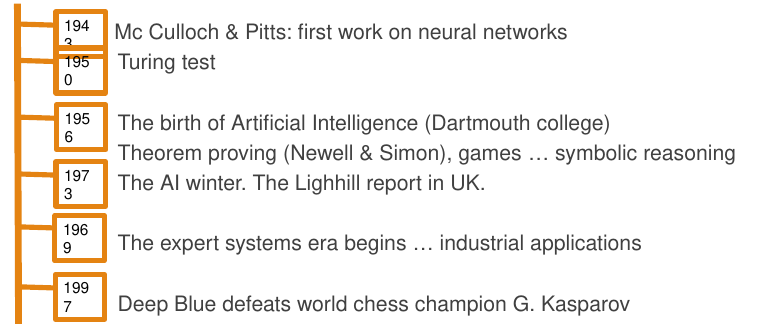
\includegraphics[width=\textwidth]{Images/timeline}
    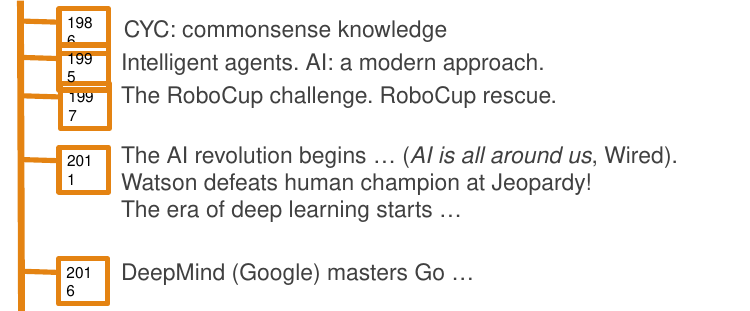
\includegraphics[width=\textwidth]{Images/timeline2}
\end{figure}
The major discover happened on $2020$ are the following:
\begin{description}
    \item [GPT3 (Generative Pre-trained Transformer): ] produced by OpenAI in May $2020$, is 
           a larger and richer language model consisting in $175$ billion machine learning parameters
           used for automatic text generation, translation, user interface synthesis
    \item [DARPA challenge (AlphaDogFights)] with simulated F-16 Air Fighters where on $18-20$ August $2020$
           there was the final Event, where AI system was against each other and the winner was a system by 
           Heron system, that was also able to defeated a human expert top gun fighter $5-0$.
\end{description}
On \cite{andrewNg} Andrew NG says that AI will transform many industries, but it’s not magic and 
almost all of AI’s recent progress is based on one type of AI, in which some input data $(A)$ is used to
quickly generate some simple response $(B)$ [$A \to B$].\newline
Also Andrew Ng says that if a typical person can do a mental task with less than one second of thought,
we can probably automate it using AI either now or in the near future.\newline
Choosing A and B creatively has already revolutionized many industries, it is poised to
revolutionize many more.

ML systems are not (yet?) able to justify in human terms their results, so for some application it is essential
the human knowledge to be able to generate explanations, infact some regulations requires the right
to an explanation in decision-making, and seek to prevent discrimination based on race, opinions,
health, sex and so on, like GPDR.\newline
ML systems learn what’s in the data, without understanding what's true or false, real or imaginary, 
fair or unfair and so it is possible to develop bad/unfair models.

The goal of building AI systems is far from being solved and is still quite challenging in its own.
Building complex AI systems requires the combination of several techniques and approaches, not only ML.\newline
One of the most challenging tasks ahead of us is integration of
perception and reasoning in AI systems.

AI fundamentals is mostly about “Slow thinking” or “Reasoning” and AI fundamentals has the role,
within the AI curriculum, of teaching you about the foundations of a discipline which is now 60 year old.\newline
We will cover different approaches, also some coming of the “Good Old-
Fashioned Artificial Intelligence” (GOFAI) or symbolic AI.

\begin{defi}
Symbolic AI is an high-level "symbolic" (human-readable) representations of problems, the 
general paradigm of searching for a solution, knowledge representation and reasoning, planning.\newline
Symbolic AI was the dominant paradigm of AI research from the mid 1950s until the late 1980s and 
central to the building of AI systems is the \emph{Physical symbol systems hypothesis}, formulated by Newell and Simon.
\end{defi}

The approach is based on the assumption that many aspects of intelligence can be achieved by the 
manipulation of symbols (the physical symbol system hypothesis):
\begin{defi}
A physical symbol system has the necessary and sufficient means for general intelligent action
\end{defi}%CITE WHO SAYS THAT
Human thinking is a kind of symbol manipulation system (a symbol system is necessary for intelligence) and 
machines can be intelligent (a symbol system is sufficient for intelligence).\newline
The hypothesis cannot be proven, we can only collect empirical evidence and observations and experiments
on human behavior in tasks requiring intelligence.

We have two different typologies of AI, that was introduced and considered:
\begin{description}
    \item [Strong AI: ] relies on the strong assumption that human intelligence can be reproduced
                        in all its aspects (general A.I.).\newline
                        It includes adaptivity, learning, consciousness and not only pre-programmed behavior.
    \item [Weak AI: ]   simulation of human-like behavior, without effective thinking/understanding and 
                        no claim that it works like human mind; it is the dominant approach today.
\end{description}
A problem of AI is that computer can't have needs, cravings or desires and Abraham Maslow's define 
a hierarchy of human needs:
\begin{enumerate}
    \item Biological needs (food, sleep, sex, ...)
    \item Safety, protection from environment
    \item Love and belonging, friendship
    \item Self esteem and respect from others
    \item Self-actualization
\end{enumerate}
%Introduction Chapter
  \chapter{Agents}
Artificial intelligence, or AI, is the field that studies the synthesis and analysis of computational agents
that act intelligently.\newline
An agent is something that acts in an environment/it does something and we are interested in what an agent does,
that is, how it acts, so we judge an agent by its actions.

An agent acts \emph{intelligently} when what it does is appropriate given the circumstances and its goals,
it is flexible to changing environments and changing goals, it learns from experience and 
it makes appropriate choices given its perceptual and computational limitations.

\begin{defi}
A \emph{computational agent} is an agent whose decisions about its actions can be explained 
in terms of computation.
\end{defi}
We have that the central scientific goal of AI is to understand the principles that make intelligent behavior
possible in natural or artificial systems, instead the central engineering goal of AI is the design and synthesis of
useful, intelligent artefacts, agents, that are useful in many applications.\newline
This is done by the analysis of natural and artificial agents, formulating and testing hypotheses about
what it takes to construct intelligent agents and in the end designing, building, and experimenting
with computational systems that perform tasks commonly viewed as requiring intelligence.

Artificial Intelligence is not the opposite of real Intelligence, infact intelligence cannot be fake, so
if an artificial agent behaves intelligently, it is intelligent and it is only the external behavior
that defines intelligence (weak AI).

Artificial intelligence is real intelligence created artificially and we can use different test to 
estabilish if AI is intelligent: \emph{Turing test} where only external behavior counts and \emph{Winograd schemas}
as a test of intelligence, where we asks "The city councilmen refused the demonstrators a permit 
because they feared violence. Who feared violence?" and "The city councilmen refused the demonstrators a permit
because they advocated violence. Who advocated violence?".\newline
These questions are difficult for a machine because it has not the knowledge of context.

The obvious naturally intelligent agent is the human being and the human intelligence
comes from three main sources:
\begin{enumerate}
    \item biology: Humans have evolved into adaptable animals that can survive in various habitats.
    \item culture: Culture provides not only language, but also useful tools, useful concepts, and 
          the wisdom that is passed from parents and teachers to children.\newline
          Language, which is part of culture, provides distinctions in the world that should be noticed for learning.
    \item life-long learning (experience): Humans learn throughout their life and accumulate knowledge and skills.
\end{enumerate}
Another form of intelligence is \emph{social intelligence}, the one exhibited by communities and organizations.

Three aspects of computation that must be distinguished:
\begin{enumerate}
    \item Design time computation, that goes into the design of the agent
    \item Offline computation, that the agent can do before acting in the world
    \item Online computation, the computation that is done by the agent as it is acting.
\end{enumerate}
Designing an intelligent agent that can adapt to complex environments and changing goals is a major challenge, so 
to reach this ultimate goal, two strategies are possible:
\begin{enumerate}
    \item simplify environments and build complex reasoning systems for these simple environments.
    \item build simple agents for natural/complex environments, simplifying the tasks.
\end{enumerate}
The design process of an agents has the following phases, that can be viewed on figure \ref{img:designProcess}:
\begin{enumerate}
    \item Define the task: specify what needs to be computed
    \item Define what constitutes a \emph{solution} and its quality: optimal solution,
          satisficing solution, approximately optimal solution, probable solution.
    \item Choose a formal representation for the task; this means choosing how to represent knowledge for the task
          and this includes representations suitable for learning.
    \item Compute an output
    \item Interpret output as a solution
\end{enumerate}

\begin{figure}
    \caption{Design Process of AI agents}
    \label{img:designProcess}
    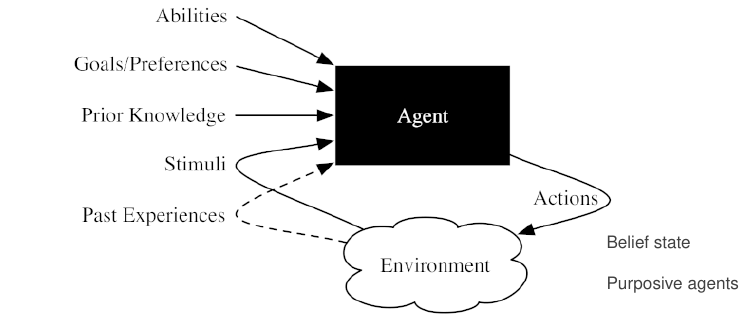
\includegraphics[width=\textwidth]{Images/agents}
\end{figure}
A model of the world is a symbolic representation of the beliefs of the agents about the world, 
so it is necessarily an abstraction.\newline
More abstract representations are simpler and human-understandable, but they
may be not effective enough and low level descriptions are more detailed and accurate but introduce complexity.

Multiple level of abstractions are possible (hierarchical design), but usually two levels are considered:
\begin{enumerate}
    \item The \emph{knowledge level}: what the agent knows and its goals
    \item The \emph{symbol level}: the internal representation and reasoning algorithms
\end{enumerate}

In agent design we consider these aspects, with a summary foundable in figure \ref{img:summary}:
\begin{description}
    \item [Modularity: ] is the extent to which a system can be decomposed into interacting modules
                         and it is a key factor for reducing complexity.\newline
                         In the modularity dimension, an agent’s structure is one of the following:
                         \begin{itemize}
                            \item \emph{flat} where there is no organizational structure.
                            \item \emph{modular}, which the system is decomposed into interacting modules
                                  that can be understood on their own.
                            \item \emph{hierarchical}, which the system is modular, and the modules themselves are
                                  decomposed into simpler modules and the agent reasons at 
                                  multiple levels of abstraction.
                        \end{itemize}

    \item [Planning Horizon: ] is how far ahead in time the agent plans and in this dimension an agent
                               is one of the following:
                               \begin{itemize}
                                    \item \emph{Non-planning agent}, that does not look at the future.
                                    \item \emph{Finite horizon} planner, where agent looks for a fixed finite
                                          number of stages and it is greedy if only looks one time step ahead.
                                    \item \emph{Indefinite horizon} planner is an agent that looks ahead some finite,
                                          but not predetermined, number of stages.
                                    \item \emph{Infinite horizon} planner is an agent that keeps planning forever
                               \end{itemize}
    \item [Representation: ] concerns on how the state of the world is described and a state of the world
                             specifies the agent’s internal state (its belief state) and the environment state.\newline
                             We have $3$ type of representation, from simple to complex:
                             \begin{itemize}
                                \item \emph{atomic} states, as in problem solving.
                                \item \emph{feature-based} representation: set of propositions that are true or
                                      false of the state, properties with a set of possible values. 
                                \item Individuals and relations (often called relational representations) and 
                                      is the Representations at the expressive level of FOL (or contractions).
                             \end{itemize}

    \item [Computational limit: ] an agent must decide on its best action within time constraints or other
                                  constraints in computational resources (memory, precision, \dots).\newline
                                  The computational limits dimension determines whether an agent has
                                  \emph{perfect rationality}, where an agent is able to reasons about the best action
                                  without constraints and \emph{bounded rationality}, where an agent decides
                                  on the best action that it can find given its computational limitations.\newline
                                  An \emph{anytime algorithm} is an algorithm where the solution quality improves
                                  with time and to take into account bounded rationality, an agent must decide
                                  whether it should act or reason for longer.

    \item [Learning: ] is necessary when the designer does not have a good model and the learning dimension 
                       determines whether knowledge is given in advance or knowledge is learned from data or 
                       past experience.\newline
                       Learning typically means finding the best model that fits the data and
                       produces a good predictive model and in this course only modelling formalisms
                       and approaches are dealt, infact all the issues concerned with learning
                       are dealt in the Machine Learning course.

    \item [Uncertainty: ] is divided into two dimensions:
                          \begin{enumerate}
                            \item uncertainty from sensing/perception (fully observable, partially observable states).
                            \item uncertainty about the effects of actions (deterministic, stochastic) and 
                            when the effect is stochastic, there is only a probability distribution
                            over the resulting states.
                          \end{enumerate}
    \item [Preference: ] considers whether the agent has goals or richer preferences:
                         \begin{itemize}
                            \item A \emph{goal} is either an achievement goal, which is a proposition to be true
                                  in some final state, or a maintenance goal, a proposition that 
                                  must be true in all visited states.
                            \item \emph{Complex preferences} involve trade-offs among the desirability of
                                  various outcomes, perhaps at different times.\newline
                                  An \emph{ordinal preference} is where only the ordering of the preferences is
                                  important, instead a \emph{cardinal preference} is where the 
                                  magnitude of the values matters and States are evaluated by utility functions.
                         \end{itemize}

    \item [Number of Agents: ] considers whether the agent explicitly considers other agents:
                               \begin{itemize}
                                    \item \emph{Single agent} reasoning means the agent assumes that there are no
                                          other agents in the environment or that all other agents are 
                                          “part of nature”, and so are non-purposive.
                                    \item \emph{Multiple agent} reasoning means the agent
                                          takes the reasoning of other agents into account and this occurs when
                                          there are other intelligent agents whose goals or preferences depend,
                                          in part, on what the agent does or if the agent must communicate
                                          with other agents.
                               \end{itemize}

    \item [Interaction: ] considers whether the agent does:
                          \begin{itemize}
                            \item \emph{offline reasoning}, where the agent determines what to do before
                                  interacting with the environment.
                            \item \emph{online reasoning}, where the agent must determine what action to do 
                                  while interacting in the environment, and needs to make timely decisions.
                          \end{itemize}
                          More sophisticated agents reason while acting and this includes long-range
                          strategic reasoning as well as reasoning for reacting in a timely manner to
                          the environment.
\end{description}

\begin{figure}
    \caption{Summary of Agent Design consideration}
    \label{img:summary}
    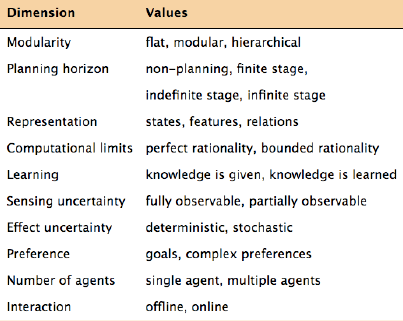
\includegraphics[width=\textwidth]{Images/summary}
\end{figure}

\begin{defi}
An agent is something that interacts with an environment, receiving information through its sensors and
acts in the world through actuators (effectors).\newline
A robot is an artificial purposive embodied agent and also a computer program is a software agent
\end{defi}
An agent is made up of a body and a controller, where the controller receives percepts from the body and
sends commands to the body.\newline
A body includes sensors that convert stimuli into percepts and actuators that convert commands into actions.
Both sensor and actuators can be uncertain, the controller is the brain of an agent and in the end
an agent system includes an agent and the environment in which it acts.\newline
In figure \ref{img:agentSystem} is possible to see the structure of an generic agent system.

\begin{figure}
    \caption{Structure of an generic agent system}
    \label{img:agentSystem}
    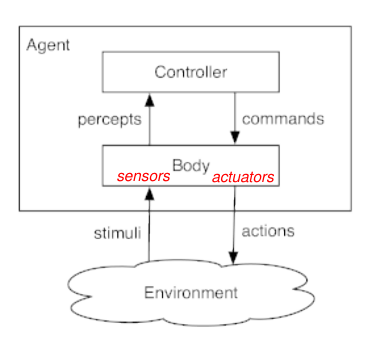
\includegraphics[width=\textwidth]{Images/agent}
\end{figure}

Agents act in time, we have $T$ that is the set of time points, and we assume that $T$ has a start $(0)$
totally ordered, discrete, and each $t$ has a next time $t + 1$.\newline
We have an agent history that at time $t$ has percepts up to $t$ and commands up to $t - 1$ and we 
have also \emph{causal transduction} (usually implements by a controller), a function from history to commands,
called causal because only previous and current percepts and previous commands can be considered.

However, complete history is usually not available and we have only the memory of it:
the memory or belief state of an agent at time $t$ is all the information the agent
has remembered from the previous times and the behavior of an agent is described by two functions:
\begin{itemize}
    \item A \emph{belief state} transition function $S \times P \to S$, where $S$ is the set of belief states 
          and $P$ is the set of percepts.
    \item A \emph{command} function $S \times P \to C$, where $C$ is the set of commands.
\end{itemize}
The controller implements a command function (an approximation of a causal transduction) and 
with a single controller it is difficult to reconcile the slow reasoning about complex high-level goals
with the fast reaction that an agent needs for lower-level tasks such as avoiding obstacles.\newline
In figure \ref{img:agentFunctions} is possible to note the agent functions that should be implemented 
at each layer of our agent.

\begin{figure}
    \caption{Agent Functions to implement at each layer}
    \label{img:agentFunctions}
    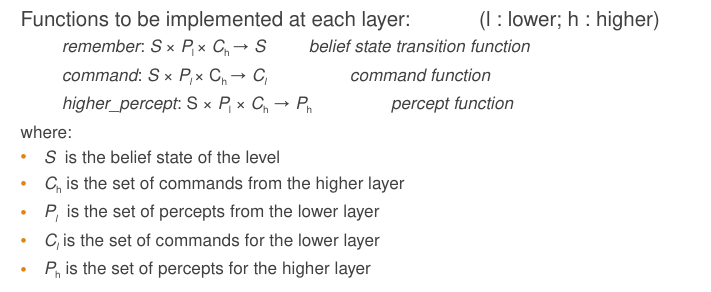
\includegraphics[width=\textwidth]{Images/agentFunctions}
\end{figure}
high-level reasoning, is often discrete and qualitative
• low-level reasoning is often continuous and quantitative
A controller that reasons in terms of both discrete and continuous values
is called a hybrid system.

The notion of belief state is quite general, most agents need to keep a model of the word and update it while acting
and there are $2$ extremes:
\begin{enumerate}
    \item the agent possess a very good predictive model, so it does not need to use perceptions to update the model
    \item purely reactive systems do not have a model, and decide only on the basis of perceptions
\end{enumerate}
In the general case the agent uses a combination of prediction and sensing:
\begin{itemize}
    \item In Bayesian reasoning (under uncertain information) the estimation
          of the next belief state is called \emph{filtering}.
    \item In alternative, more complex models of the world can be kept and updated, for
          example through vision and image processing.
\end{itemize}
Knowledge of a specific domain may also be represented explicitly and used to decide the action and 
the \emph{knowledge base} contains general rules and specific/contingent facts in declarative form.\newline
The KB is built offline, built by designers or learned from data and a domain ontology gives meaning
to symbols used to represent knowledge; knowledge may be then updated and used to decide actions during
operation.






%Agent Chapter
  \chapter{CSP (Constraint Satisfaction Problems}
It is often better to describe states in terms of features and then to reason in terms of these features and we have called this a \emph{factored representation}.

This representation may be more natural and efficient than explicitly enumerating the states, so with $10$ binary features we can describe $2^10 = 1024$ states,
often these features are not independent and there are constraints that specify legal combinations of assignments of values to them.

A CSP is a problem composed of a finite set of variables, each variable is associated with a finite domain and a set of constraints that restrict the values
the variables can simultaneously take, so the task is to assign a value (from the associated domain) to each variable satisfying all the constraints;
this problem is in NP hard in the worst cases but general heuristics exist, and structure can be exploited for efficiency.

A Constraint Satisfaction Problem consists of three components, $X, D,$ and $C$, so $CSP = (X, D, C)$ where 
$X$ is a set of variables $\{x_1, \dots, x_n\}$, $D$ is a set of domains $\{D_1, \dots, D_n\}$, one for each variable, and 
$C$ is a set of contraints that specify allowable combinations of values.

A [partial] assignment of values to a set of variables (also called compound label) is a set of pairs $A = \{(x_i, v_i), (x_i, v_j), \dots\}$
where values are taken from the variable domain and we have that a complete assignment is an assignment to all the variables of the problem (a possible world).\newline
A complete assignment can be projected to a smaller partial assignment by restricting the variables to a subset and we will use the projection operator 
from relational algebra as notation.

A constraint on a set of variables is a set of possible assignments for those variables and each constraint C can be represented as a pair (scope, rel), 
where scope is a tuple of variables participating in the constraint $(x_1, x_2, \dots, x_k)$ and rel is a relation that defines the allowable combinations 
of values for those variables, taken from their respective domains.

To solve a CSP problem $(X, D, C)$, seen as a search problem, we need to define a state space and the notion of a solution:
a state in a CSP is an assignment of values to some or all of the variables and we have a partial assignment when we assigns values to only some of the variables,
a complete assignment when every variable is assigned and in the end a consistent assignment is the one that satisfies all the constraints.\newline
A solution to a CSP (a goal state) is a consistent, complete assignment.

%The simplest kind of CSP involves variables that have discrete, finite domains
% Values can be numbers, strings, Booleans (True, False)
%When variables are numbers, and the constraints are inequalities we can deal with
%variables with infinite domains or continuous domains with linear or integer
%programming (techniques used in Operations research).
%According to the number of variables involved constraints can be:
% unary (ex. “x even”)
% binary (ex. “x  y”)
% higher-order constraints (ex. x+y = z)
%Absolute/hard vs soft/preference constraints
% CSPs with preferences can be solved by optimization methods. These are called
%Constraint Optimization Problems, or COP.

%Problem reduction/Inference/Constraint propagation
% Techniques for transforming a CSP into an equivalent one which is easier to solve or
%recognizable as insoluble (removing values from domains and tightening constraints).
%Searching
% Search in the space of labels: enumerate combinations of labels to find solutions.
% How to search efficiently: heuristics, intelligent backtracking ... local search
%Exploiting the structure of the problem
% Independent sub-problems, tree-structured constraints, tree-decomposition,
%exploiting symmetry
%CSP Chapter
  \chapter{Knowledge representation \& reasoning}
We introduce and discuss about Knowledge representation and Reasoning (KR \& R), that
is the field of Artificial Intelligence dedicated to representing information about the 
world in a form that a computer system can utilize to solve complex tasks.

The class of systems that derive from this approach are \emph{knowledge based agents} and
a KB agent maintains a knowledge base of facts expressed in a declarative language.

A representation is a surrogate for reasoning about things that exists externally,
it is necessarily imperfect, it is also a set of ontological commitments and a fragmentary
theory of intelligent reasoning.

Knowledge representation is about the use of formal symbolic structures to represent a 
collection of propositions believed by some agent, instead reasoning is the formal
manipulation of the symbols representing a collection of beliefs to produce representations
of new ones, so logical deduction is a well know example of reasoning.

Reasoning is not only done by logical entailment/deduction but we have also default reasoning, probabilistic reasoning and so on, that we will introduce later in this chapter.

The Knowledge Representation hypothesis formulated by Brian C. Smith in 1985 estabilish 
that any mechanically embodied intelligent process will be comprised of structural
 ingredients that:
\begin{itemize}
   \item we as external observers naturally take to represent a propositional account
         of the knowledge that the overall process exhibits.
   \item independent of such external semantic attribution, play a formal but causal
         and essential role in engendering the behavior that manifests that knowledge.
\end{itemize}
In simpler words, we want to construct A.I. systems that contain symbolic
representations that we can understand these symbolic structures as propositions and 
these symbolic structures determine the behavior of the system; we have that 
Knowledge based systems have these properties.

There are two competing approaches for KB systems:
\begin{description}
    \item [Procedural approach: ] knowledge is embedded in programs.
    \item [Connectionist approach: ] avoids symbolic representation and reasoning, and 
           instead sees computing with networks of weighted links between "neurons".
\end{description}
The KB approach has the following advantages:
\begin{enumerate}
   \item Separation of knowledge and "inference engine".
   \item Extensibility: we can extend the existing behavior by simply adding new 
         propositions and the knowledge is modular, so the reasoning mechanism
         does not change.
   \item Understandability: the system can be understood at the knowledge level,
         so we debug faulty behavior by changing erroneous beliefs, and we can explain
         and justify current behaviour in terms of the beliefs.
\end{enumerate}
There is a fundamental tradeoff in knowledg representation and reasoning who estabilish
that the more expressive is the representation language, the more complex is reasoning.

So we need to find a best compremise between this two aspects, so for example databases
use only positive and concrete facts and also FOL avoid to represent some default aspects.

Much of AI involves building systems that are knowledge-based: their ability derives [in
part] from reasoning over explicitly represented knowledge and typical KB systems are
expert systems, language understanding, machine reading (common sense knowledge is required)and planning; KR\&R today has many applications outside AI, like Bio-medicine,
Engineering, Business and commerce, Databases, Software engineering.

We will consider two "modern" applications:
\begin{itemize}
   \item Cognitive assistants/digital personal assistants (SIRI/Alexa/Google home/Jibo),
	 spoken dialog in a natural language in open domain.
   \item Computational Knowledge Engine (Wolfram Alpha): scientific and medical thinking.
\end{itemize}
\section{Proposizional and First Order Logic}
We can understand KB systems at two different levels:
\begin{description}
    \item [Knowledge level: ] representation language and its semantics, 
	   expressive adequacy (what can be expressed), and what can be inferred.
    \item [Symbol level: ] computational aspects, efficiency of encoding, data structures
	    and efficiency of reasoning procedures, including their complexity.
\end{description}
The tools of symbolic logic seem especially suited for the knowledge level.

We have that a sentence is true (or false) with respect to an interpretation, where
an interpretation (possible world) assigns truth values to atomic formulas.

Truth values of compound formulas follow as a consequence and an interpretation that makes
a set of formulas true, is called a model.\newline
A formula is satisfiable if there is at least one interpretation that makes it true and 
unsatisfiable if is false in all interpretations.\newline
A formula is valid (a tautology in PROP) if it is true in all interpretations and note that
the negation of a satisfiable formula can be satisfiable or unsatisfiable and 
the negation of a valid formula is unsatisfiable, and vice versa.

A set of sentences KB [logically] entails a sentence $\alpha$ iff any model of KB is
also a model of $\alpha$ and we also say that $\alpha$ is a logical consequence of KB.

We write $KB \models \alpha$ and we have an alternative definition that says
\[ KB \models \alpha \iff M(KB) \subseteq M(\alpha) \]
where $M$ stands for the set of models; it is also possible define the logical equivalence
as $\alpha \equiv \beta$ iff $\alpha \models \beta$ and $\beta \models \alpha$.

A deductive system is defined by a set of axioms and inference rules and axioms can be
logical or part of the agent’s KB.\newline
A proof is a sequence of formulas, starting from the axioms, where each formula can
be obtained from previous ones by application of inference rules and 
we write $KB \vdash \alpha$ when there is a proof of $\alpha$ from KB.

We have connection between deduction and entailment with these two definition:
\begin{description}
    \item [Soundness: ] if $KB \vdash \alpha$ then $KB \models \alpha$.
    \item [Completeness: ] if $KB \models \alpha$ then $KB \vdash \alpha$.
\end{description}
Proof by refutation is based on the following meta-theorem
$KB \models \alpha$ iff $KB \cup \{\neg \alpha\}$ is unsatisfiable, and this means that
entailment can be formulated as a satisfiability problem (SAT): we can use SAT
algorithms for checking entailment and if $KB \cup \{\not \alpha \}$ derives a 
contradiction, and the proof system is sound, then $KB \models \alpha$.

It is possible to convert any finite domain CSP into a propositional satisfiability
problem, so if $Y$ has domain $\{v_1, \dots, v_k\}$ introduce $k$ boolean variables
$Y_1 , \dots, Y_k$, with $Y_i$ iff $Y = v_i$.\newline
Additional constraints are that if at least one of $Y_1, \dots, Y_k$ is true and 
if $i \neq j$ then $Y_i$ and $Y_j$ not both true and we define a clause for each disallowed
combination of values $(v_1, \dots, v_k): \{\neg v_1 \lor \dots \lor \neg v_k \}$.

Satisfiability (SAT) algorithms for PROP can be made more efficient than general CSP
solvers and strategies for computing entailment in PROP:
\begin{enumerate}
   \item Model checking (reduce to SAT problem) that consist in several approach:
	 check satisfiability using different heuristics (DPLL) or 
	 use a local and incomplete search method (Walk-SAT).
   \item Deduction (uses a proof system and deduction strategies): the resolution method
	   uses only one inference rule (resolution rule) and resolution strategies
         for searching are more efficiently.
\end{enumerate}
Clausal form (PROP) is a Conjunctive normal form (a conjunction of disjunctions
of atomic formulas) and any PROP formula can be converted in an equivalent set of
clauses: each conjunct is a clause, a disjunction of literals (positive o negative atoms).

DPLL (Davis, Putman, Lovemann, Loveland) requires a formula in clausal form and it 
enumerates, with a depth first strategy, all interpretations, looking for a model.\newline
It uses three strategies:
\begin{enumerate}
   \item Anticipated control, so if one clause is false backtrack or if one literal
	 is true the clause is satisfied.
   \item Pure symbols heuristics, where assign first pure symbols (which appear 
	 everywhere with the same sign).
   \item Unit clauses heuristics, which assign first unit clauses (only one literal).
\end{enumerate}
In figure \ref{img:dpllPseudo} is possible to note the pseudocode of DPLL.

\begin{figure}
	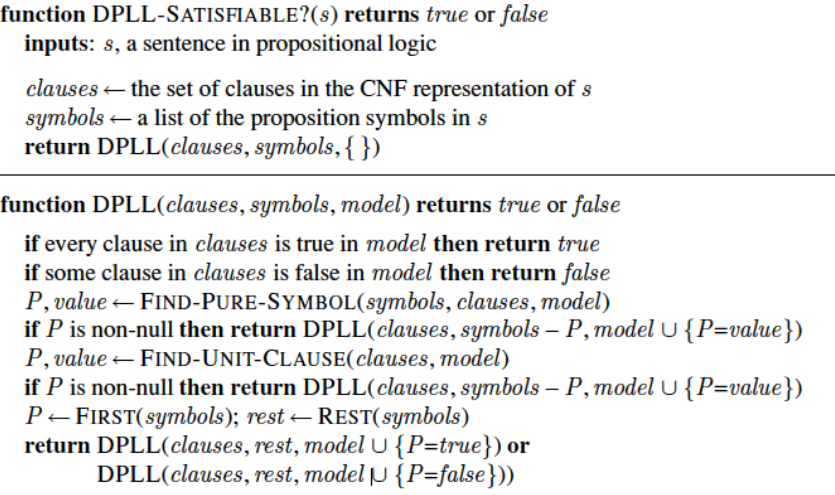
\includegraphics[width=\textwidth]{Images/dpll}
	\caption{Pseudocode of DPLL}
	\label{img:dpllPseudo}
\end{figure}

Walk-SAT is one (of many) local search methods and is to be used for SAT problems
where solutions exist and are evenly distributed; it is not complete and is 
very effective for large problems.

In figure \ref{img:walkSat} is possible to note the pseudocode to compute Walk-Sat and 
in figure \ref{img:comparisonDPLL} is possible to see a comparison between DPLL and WalkSat.

\begin{figure}
	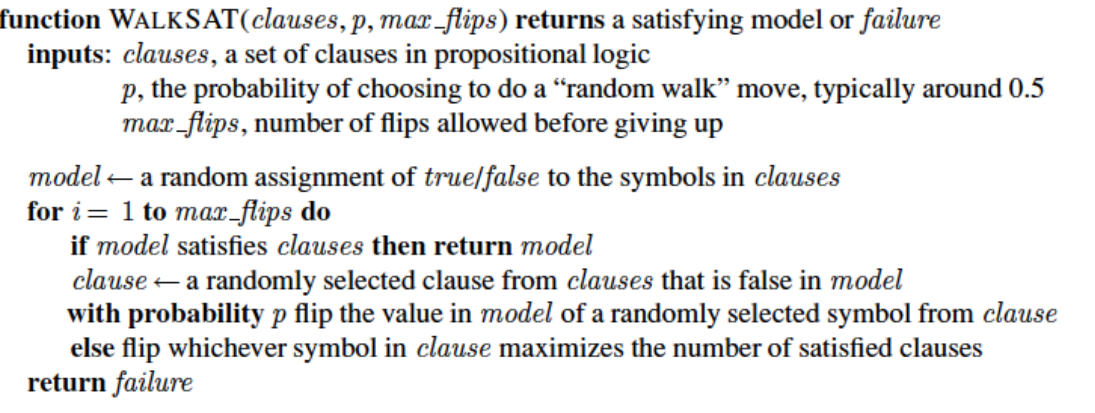
\includegraphics[width=\textwidth]{Images/walksat}
	\caption{Pseudocode of WalkSat}
	\label{img:walkSat}
\end{figure}

\begin{figure}
	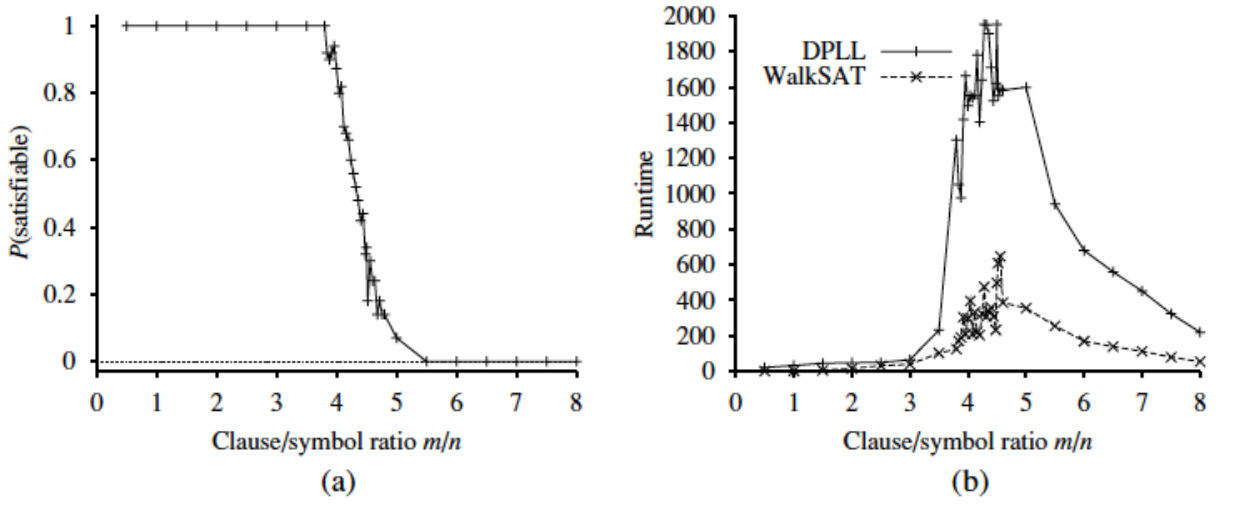
\includegraphics[width=\textwidth]{Images/dpllComparison}
	\caption{Comparison between DPLL and WalkSat}
	\label{img:comparisonDPLL}
\end{figure}
Also in the case of FOL you can obtain a clausal form in an effective way, and the 
transformation involves the elimination of existential quantifiers by Skolemization, so
\[ \exists x father(x, G) \text{ becomes } father(k, G) \]
This transformation preserves satisfiability, but not equivalence.

Given the fundamental problem $KB \models \alpha$ an equivalent problem is
$KB \cup \neg \alpha$ is unsatisfiable and this can be solved by a deductive system
showing that $KB \cup \neg \alpha \vdash \{ \}$, where $\{ \}$ is the
empty clause meaning False.

Resolution by refutation is a method which is correct and complete:
\begin{enumerate}
   \item transform the KB in clausal form (a conjunction of disjunction of literals)
   \item add to KB the negation of the goal in clausal form
   \item use the resolution rule as unique inference rule.
\end{enumerate}
This strategy works for PROP and FOL with different complexity results:
it is decidable and NP-complete for PROP, instead is semi-decidable for FOL.

Clauses are set of literals, so the resolution rule for PROP is the following
\[ \frac{c_1 \cup \{p\} \, \, \, \, c_2 \cup \{\neg p\}} {c_1 \cup c_2} \]
In a resolution refutation we aim to deduce the empty clause and the resolution rule
for FOL is the following:
\[ \frac{c_1 \cup \{ p \} \, \, \, \, c_2 \cup \{\neg q\}} {[c_1 \cup c_2]\gamma} \]
and $\gamma = MGU(p, q)$ and $\gamma$ is not fail, so a fundamental operation is 
\emph{unification}, who is a process to determine whether two expressions can be made
identical by a substitution of terms to variables, so 
the result is the unifying substitution, the unifier, or FAIL,
if the expressions are not unifiable.

Given two expressions there may be different substitutions that make them identical and 
we are interested in computing the most general unifier (MGU), the one that does only
the essential instantiations.

We present now the Unification algorithm, invented in $1982$ by Martelli and Montanari,
which consist in the following passes:
\begin{enumerate}
   \item Computes the MGU by means of a rule-based equation-rewriting system
   \item Initially the working memory (WM) contains the equality of the two
         expressions to be unified.
   \item The rules modify equations in the WM
   \item The algorithm terminates with failure or when there are no applicable rules
	 (success)
   \item At the end, if there is no failure, the WM contains the MGU.
\end{enumerate}
The rules used to compute the MGU are the following:
\begin{enumerate}
   \item $f(s_1, \dots, s_n) = f(t_1, \dots, t_n) \to s_1 =  t_1 , \dots, s_n = t_n$
   \item $f(s_1, \dots, s_n) = g(t_1, \dots, t_m) \to fail$ when $f \neq g$ or $n \neq m$.
   \item $x = x$ we can remove the equation
   \item $t = x \to x = t$ 
   \item $x = t, x$ does not occur in $t$ the nwe apply $\{x/t\}$ to other equations.
   \item $x = t, t$ is not $x$, $x$ occur in $t$ then we have fail.
\end{enumerate}
Note that when we compare two different constants, rule 2 applies, as a special case
where $n = m = 0$, and we fail.

\section{Knowledge \& Ontological Engineering}
\emph{Knowledge engineering} is the activity to formalize a specific problem or
task domain and it involves decisions about what are the relevant fact, objects and so on,
but also which is the right level of abstaction.\newline
\emph{Ontology engineering} seeks to build general-purpose ontologies which should be
applicable in any special-purpose domain (with the addition of domain-specific axioms). 

Before implementing, need to understand clearly, like in software engineering
what is to be computed, what kind of knowledge, why and where inference is necessary.

Sometimes useful to reduce n-ary predicates to 1-place predicates and 1-place functions,
that involves creating new individuals and new functions for properties/roles,
this is typical of description logics/frame languages, which we will talking later.

The use of KR languages and logic in A.I. is representing “common sense”
knowledge about the world, rather than mathematics or properties of programs.\newline
Common sense knowledge is difficult since it comes in different varieties and it
requires formalisms able to represent actions, events, time, physical objects, beliefs,
categories that occur in many different domains.

In figure \ref{img:general} is possible to note that a general ontology organizes 
everything in the world into a hierarchy of categories and should be applicable
in any special-purpose domain (with the addition of domain-specific axioms).\newline
In any non trivial domain, different areas of knowledge must be combined,
because reasoning and problem solving could involve several areas simultaneously and 
it is difficult to construct one best ontology, infact "Every ontology is a treaty—a
social agreement—among people with some common interest in sharing.”

\begin{figure}
	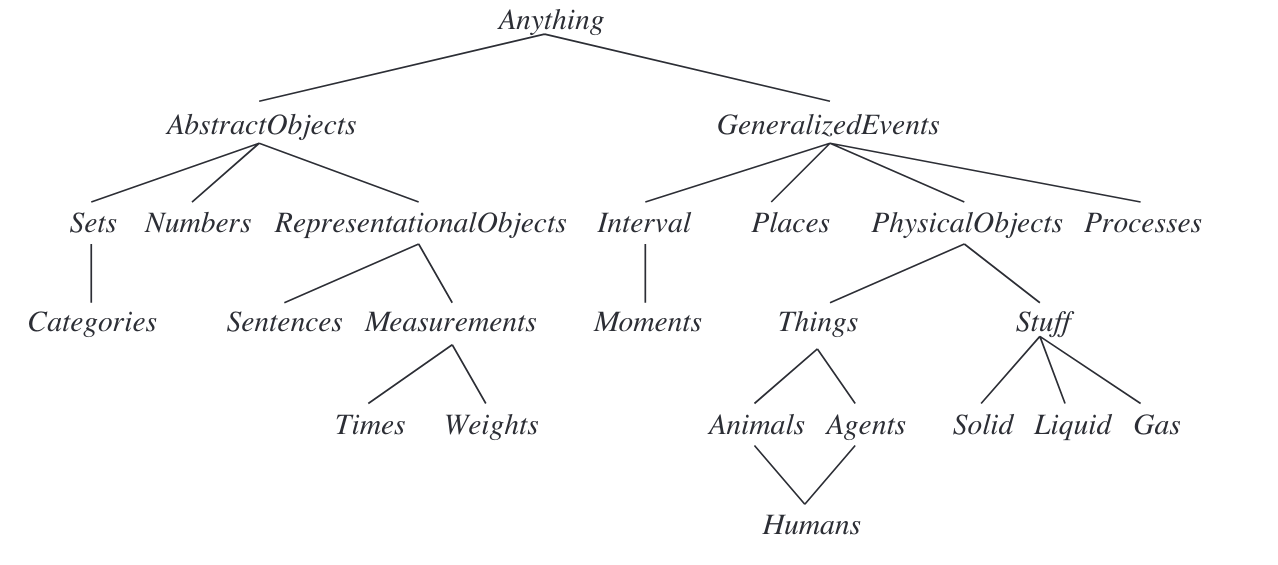
\includegraphics[width=\textwidth]{Images/generalOntology}
	\caption{General Ontology specification}
	\label{img:general}
\end{figure}
Much reasoning takes place at the level of categories, so we can infer category
membership from the perceived properties of an object, and then uses category
information to derive specific properties of the object.\newline
There are two choices for representing categories in first-order logic:
\begin{enumerate}
    \item Predicates, categories are unary predicates, that we assert of individuals:
    \item Objects: categories are objects that we talk about (\emph{reification}),
	  so for example the predicate $WinterSport(Ski)$ become $Ski \in WinterSports$
\end{enumerate}
In this way we can organize categories in taxonomies (like in natural sciences),
define disjoint categories, partitions and use specialized inference mechanisms,
such as inheritance. 

We use the general PartOf relation to say that one thing is part of another,
composite objects can be seen as part-of hierarchies, similar to the Subset hierarchy
and these are called \emph{mereological hierarchies}.

Composite objects is a structural relations among parts so 
for example, a biped has two legs attached to a body will be represented as a relation
among biped and leg.

\emph{Bunch} is a composite objects with definite parts but no particular structure,
so "a bag of three apples" will be represented by BunchOf($\{Apple_1, Apple_2, Apple_3\})$
that should not be confused with the set of $3$ apples and unlike sets, bunches have
weight; also we have that each element of category $s$ is part of BunchOf(s) and also
BunchOf(s) is the smallest object satisfying this condition (logical minimization).

Physical objects have height, weight, mass, cost, and so on and the values that we
assign for these properties are called measures.\newline
A solution is to represent measures with units functions that take a number as argument
so for example we have Length($L_1$) = Inches($1.5$) = Centimeters($3.81$).\newline
The most important aspect of measures is not the particular numerical
values/scale, but the fact that measures can be ordered, and to perform some sort
of qualitative inference, often it is enough to be able to order values 
and to compare quantities (qualitative physics).

There are countable objects, things such as apples, holes, and theorems, and
mass objects, such as butter, water, and energy, these are called Stuff.\newline
The properties of stuff are the following:
\begin{enumerate}
  \item Any part of butter is still butter, so we have in symbols
	\[ b \in  Butter \cap PartOf(p, b) \Rightarrow  p \in  Butter \]
  \item Stuff has a number of intrinsic properties (color, high-fat content, density \dots        ), shared by all its subparts, but no extrinsic properties, so it is a substance.
\end{enumerate}

\section{Situation Calculus}
The situation calculus is a specific ontology in FOL dealing with actions and change,
with the following concepts:
\begin{description}
    \item [Situations: ] snapshots of the world at a given instant of time,
	                 the result of an action.
    \item [Fluents: ]    time dependent properties.
    \item [Actions: ]    performed by an agent, but also events.
    \item [Change: ]     how the world changes as a result of actions.
\end{description}
We define Result as the effect of a sequence of actions, defined as a function
\[ Result: [A*] \times S \to S \]
with Result([], s) = s and Result([a | seq], s) = Result(seq, Result(a, s)).

The frame problem is one the most classical A.I. problems and the name comes from 
an analogy with the animation world, where the problem is to distinguish background
(the fixed part) from the foreground (things that change) from one frame to the other.
Let’s try to fix the problem writing frame axioms, such that an action remains true
unless someone makes false, but with frame axioms we have too many axioms
(representational frame problem).

We can combine preconditions, effect and frame axioms to obtain a more compact 
representation for each fluent $f$ and the schema is as follows:
$f$ true after true preconditions and some action made $f$ true or
f was true before and no action made it false.

The representational frame problem is considered to be (more or less) solved with 
this new definition and we have another problem, called \emph{Qualification problem},
since in real situations it is almost impossible to list
all the necessary and relevant preconditions.\newline
\emph{Ramification problem} is the problem of among derived propertied which ones
persist and which ones change?

What we would need is the ability to formalize a notion of persistence, that estabilish
that “in the absence of information to the contrary (by default)
things remain as they were”.\newline
Unfortunately this leads out of classical logic and the closure assumption we used 
is already an ad hoc form of completion and we will see more
of this strategy in nonmonotonic reasoning.\newline
In planning we end up using other languages that make stronger assumptions
and are more limited in their expressivity.

Situation calculus is limited in its applicability: Single agent, Actions are discrete
and instantaneous (no duration in time), Actions happen one at a time: no concurrency,
no simultaneous actions and only primitive actions, so there is no way 
to combine actions (conditionals, iterations and so on).\newline
To handle such cases we introduce an alternative formalism/ontology known as
\emph{event calculus}, which is based on events, points in time,
intervals rather than situations.

\section{Event Calculus}
Event calculus reifies fluents and events and the fluent is an object 
(represented by a function), so to assert that a fluent is true at some point
in time t we use the predicate T, so for example 
T(At(Shankar, Berkeley), t).

Events are described as instances of \emph{event categories}, so for example
the event $E_1$ of Shankar flying from San Francisco to Washington, D.C. is described as
\[ E_1 \in Flyings \cap Flyer(E_1 , Shankar) \cap Origin(E_1 , SF ) \cap 
   Destination(E_1 , DC) \]
By reifying events we make it possible to add any amount of arbitrary information
about them, such participants in the event or properties.

Time intervals are a pair of times $(start, end)$, so $i = (t_1, t_2)$
is the time interval that starts at $t_1$ and ends at $t_2$.\newline
We have the event Happens($E_1, i)$ to say that the event $E_1$ took place 
over the time interval $i$.\newline
The complete set of predicates for one version of the event calculus is the following:
\begin{description}
    \item [$T(f, t)$] fluent $f$ is true at time $t$.
    \item [Happens(e, i)] event $e$ happens over the time interval $i$.
    \item [Initiates(e, f, t)] event $e$ causes fluent $f$ to start at time $t$.
    \item [Terminates(e, f, t)] event $e$ causes fluent $f$ to cease at time $t$.
    \item [Clipped(f, i)] fluent $f$ ceases to be true at some point during 
	                  time interval $i$.
    \item [Restored(f, i)] fluent $f$ becomes true sometime during time interval $i$.
\end{description}
A fluent holds at a point in time if the fluent was initiated by an event at some
time in the past and was not made false (clipped) by an intervening event, so formally
\[ Happens(e, (t_1, t_2)) \cap Initiates(e, f, t_1) \cap \not Clipped(f, (t_1, t)) \cap
   t_1 < t \Rightarrow T(f, t) \]
A fluent does not hold at a point in time if the fluent was terminated by an event
at some time in the past and was not restored by an event occurring at a later time,
so formally we have
\[ Happens(e, (t_1, t_2)) \cap Terminates(e, f, t_1) \cap \not Restored(f, (t_1, t)) \cap
   t_1 < t \Rightarrow \not T(f, t) \]
where Clipped and Restored are defined by
\begin{align*}
	Clipped(f , (t_1 , t_2)) & \iff \exists e, t, t_3 Happens(e, (t, t_3)) \cap
	t_1 \leq t < t_2 \cap Terminates(e, f, t) \\
        Restored(f, (t_1, t_2)) & \iff \exists e, t, t_3 Happens(e , (t, t_3)) \cap
	t_1 \leq t < t_2 \cap Initiates(e, f, t) \\
\end{align*}
We can extend the predicate $T$ to hold over intervals, so we says that a fluent
holds over an interval if it is true at every point within the interval
\[ T(f, (t_1, t_2)) \iff [\forall t \, (t_1 \leq t < t_2) \Rightarrow T(f, t)] \]
Actions are modeled as events, and we have that fluents and actions are related
with domain-specific axioms that are similar to successor-state axioms.\newline
We can extend event calculus to make it possible to represent simultaneous
events, continuous events and so on.

\emph{Processes} or liquid events are events with the property that if they happen
over an interval also happen over any subinterval
\[ (e \in Processes) \cap Happens(e, (t_1, t_4)) \cap (t_1 < t_2 < t_3 < t_4)
   \Rightarrow Happens(e, (t_2, t_3)) \]
The distinction between liquid and nonliquid events is analogous to the
difference between substances, or stuff, and individual objects, or things.

We can model in detail the behavior of intervals, providing more vocabulary:
\begin{description}
   \item [Time(x)] points in a time scale, giving us absolute times in seconds.
   \item [Begin(i)] earliest moment in an interval.
   \item [End(i)] latest moment in an interval.
   \item [Duration(i)] the duration of an interval.
\end{description}
The Complete set of interval relations, proposed by Allen (1983) and visible in figure
\ref{img:timeInterval}, are the following:
\begin{itemize}
   \item $Meet(i, j) \iff End(i) = Begin(j)$
   \item $Before(i, j) \iff End(i) < Begin(j)$
   \item $After(j, i) \iff Before(i, j)$
   \item $During(i, j) \iff Begin(j) < Begin(i) < End(i) < End(j)$
   \item $Overlap(i, j) \iff Begin(i) < Begin(j) < End(i) < End(j)$
   \item $Begins(i, j) \iff Begin(i) = Begin(j)$
   \item $Finishes(i, j) \iff End(i) = End(j)$
   \item $Equals(i, j) \iff Begin(i) = Begin(j) \cap End(i) = End(j)$
\end{itemize}

\begin{figure}
	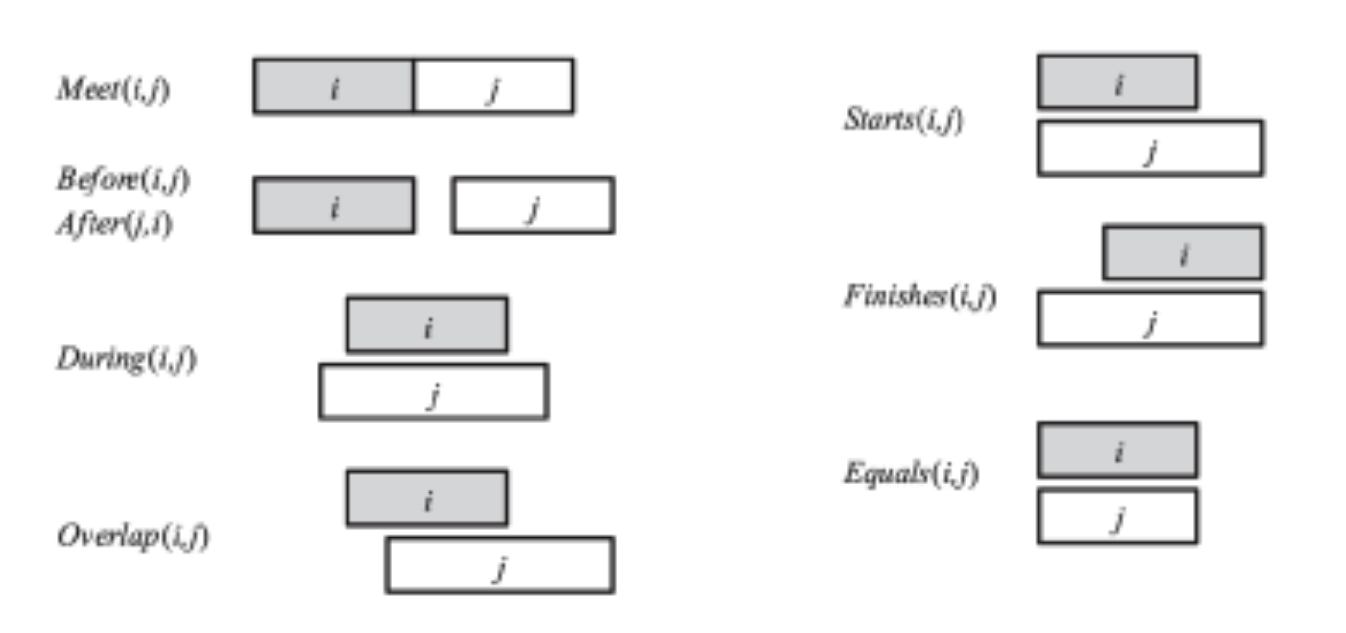
\includegraphics[width=\textwidth]{Images/intervalRelations}
	\caption{Visual representation of interval relations}
	\label{img:timeInterval}
\end{figure}

\section{Nonmonotonic reasoning}
Failures of monotonicity are widespread in commonsense reasoning, infact it seems
that humans often “jump to conclusions”, when they think it is safe to do so
(lacking information to the contrary).\newline
These conclusions are only “reasonable”, given what you know, rather than
classically entailed and also most of the inference we do is defeasible:
additional information, may lead to to retract those tentative conclusions.\newline
Any time the set of beliefs does not grow monotonically as new evidence arrives,
the monotonicity property is violated and including defeasible reasoning
leads us to consider nonsound inferences.

Some common instances of nonmonotonic reasoning are the following:
\begin{description}
   \item [Default reasoning: ] reasonable assumptions unless evidence of the contrary
   \item [Persistence: ] things stay the same, according to a principle of inertia,
	                 unless we know they change.
   \item [Economy of representation: ] only true facts are stored, false facts are only
                                       assumed.
   \item [Reasoning about knowledge:] if you have $\neg Know(p)$ and you learn $p$ we
	                              have $Know(p)$.
   \item [Abductive reasoning: ] most likely explanations to known facts.
\end{description}
Universal rules, like $\forall x (P(x) \Rightarrow Q(x))$, express properties that
apply to all instances, but most of what we learn about the world is 
in terms of generics rather than universals.\newline
Listing exceptions to generic properties is not a viable solution, so the goal is to 
be able to say a $P$ is a $Q$ in general, normally, but not necessarily.\newline
In this way it is reasonable to conclude $Q(a)$, given $P(a)$, 
unless there is a good reason not to and this is what we call a \emph{default}
and \emph{default reasoning} the tentative conclusion.

There are three ways to approach the problem, that we will analyze:
\begin{description}
   \item [Model theoretic formalizations (CWA, Circumscription):]
         consist in a restriction to the possible interpretations, 
         redefining the notion of entailment and we can still have systems
	 sound and complete wrt the new semantics.
   \item [Proof theoretic formalizations (Default logic, Autoepistemic logic):]
      A proof system with non-monotonic inference rules and autoepistemic logic
	(under the heading “logics for knowledge and beliefs”).
   \item [Systems supporting belief revision TMS, ATMS]
\end{description}
Under Closed World Assumption (CWA) only positive facts are stored, any other 
basic fact is assumed false and CWA assumption is used in [deductive] databases
and in logic programming with negation as failure.

CWA corresponds to a new version of entailment ($\models_c$) defined as 
\begin{defi}[CWA]
    $KB \models_c a$ if and only if $CWA(KB) \models a$ where 
    \[ CWA(KB) = KB \cup \{ \neg  p : \text{ p ground atom and } KB \not \models p \} \]
\end{defi}
$CWA(KB)$ is the completion under CWA of KB and note that the $CWA$ is nonmonotonic.

KB with consistent knowledge (satisfiable) happens when for no $\alpha \, KB \models \alpha$
and $KB \models \neg \alpha$, but normally a KB has incomplete knowledge.\newline
CWA can be seen as an assumption about complete knowledge, or a way to 
make a theory complete, using the following theorem:
\begin{thm}
    For every $\alpha$ (without quantifiers), $KB \models_c \alpha$ or 
$KB \models_c \neg \alpha$.
\end{thm}
$CWA(KB)$ is not always consistent when KB is consistent, infact there are problem
with disjunctions, so a solution is to restrict $CWA$ to atoms that are 
“uncontroversial”; CWA limited in such a way is called Generalized CWA (GCWA) and
is a weaker form of completion than unrestricted CWA (the assumed beliefs are less).
\begin{thm}[Consistency of CWA]
   $CWA(KB)$ is consistent iff whenever $KB \models (q_1 \vee \dots \vee q_n)$
   then $KB \models q_i$ for some $q_i$.\newline
   GCWA comes if $KB \models \{ p \vee q_1, \dots \vee q_n\}$ and $KB \not \models p$
   add $\neg p$ only if at least one ground literal $q_i$ is entailed.
\end{thm}
Since it may be difficult the condition of the theorem, the following corollary, which
restricts the application, is also of practical importance:
\begin{corol}
    If the clause form of $KB$ is Horn and consistent, then $CWA(KB)$ is consistent.
\end{corol}
The application of the theorem of consistency of $CWA$ depends on the terms 
that we allow as part of the language, and the Domain Closure Assumption (DCA) 
may be used to restrict the constants to those explicitly mentioned in the KB:
\[ \forall x. [x = c_1 \lor \dots \lor x = c_n] \]
where $c_i$ are all the finite constants appearing in KB.\newline
Under this restriction quantifiers can be replaced by finite conjunctions
and disjunctions and we also introduce the Unique Names assumption (UNA),
that can be used to deal with terms equality $c_i \neq c_j$ for $i \neq j$
but with functions things get more complicated.

With CWA we can reduce queries (without quantifiers) to atomic queries, by
repeated applications of the following properties:
\begin{enumerate}
    \item $KB \models_c (a \wedge b)$ iff $KB \models_c a$ and $KB \models_c b$
    \item $KB \models_c \neg \neg a$ iff $KB \models_c a$
    \item $KB \models_c \neg (a \vee b)$ iff 
	  $KB \models_c \neg a$ and $KB \models_c \neg b$
    \item $KB \models_c (a \vee b)$ iff $KB \models_c a$ or $KB \models_c b$
    \item $KB \models_c \neg(a \wedge b)$ iff
	  $KB \models_c \neg a$ or $KB \models_c \neg b$
\end{enumerate}
If $CWA(KB)$ is consistent, any query reduces to a set of atomic queries and we further
assume that $CWA(KB)$ is consistent we get
\[ KB \models_c \not a \iff KB \not \models_c a \] 
Much more efficient than ordinary logic reasoning (e.g. no reasoning by cases),
in fact we have restricted reasoning to a unique interpretation and instead of
checking validity/entailment we check truth in that interpretation.

In a \emph{vivid KB} we store this unique interpretation (a consistent and complete
set of literals) and answer questions retrieving from it, so a vivid KB
has the CWA builtin.\newline
If atoms are stored as a table, deciding if $KB \models_c \alpha$ is like DB-retrieval,
so instead of reasoning with sentences we reason about an analogical
representation of the world, or model.

The CWA is too strong for many applications, so we do not want to assume that any
ground atom not provable from the KB is false, because certain predicates
are considered complete, others are not.\newline
CWA wrt to a predicate P [set of predicates P]: the set of assumed beliefs is only
for ground atoms in P [predicates in P] and a similar theory is predicate completion
which consists in adding a set of completion axioms, so if only $P(A)$ and $P(B)$
are in KB we have that the completion axiom is defined as 
\[ \forall (x = a) \vee (x = b) \iff P(x) \]
The theory accounting for if and when this leads to consistent augmentation is
quite complex and a generalization of CWA and predicate completion is circumscription.

\emph{Circumscription} can be seen as a more powerful and precise version of the CWA,
working also for FOL, which was problematic and required further assumptions.\newline
The idea is to specify special abnormality predicates for dealing with exceptions and 
the definition of Circumscription is defined as 
\begin{defi}[Circumscription]
    Given the unary predicate Ab, consider only interpretations where $I[AB_f]$
    is as small as possible, relative to KB.
\end{defi}
Note that Circumscription is a semantic notion based on minimal models (a kind of
model preference logics) due to MacCarthy $1980$.

Let $P$ be a set of unary abnormality predicates and let $I_1$ and $I_2$ two 
interpretations that agree on the values of constants and functions so we define 
the ordering and minimal entailment as 
\begin{defi}[Minimal Entailment]
  $I_1 < I_2$ iff same domain and $\forall p \in P I_1[p] \subset I_2[p]$ holds and the 
  minimal entailment estabilish that $KB \models _{\leq} \alpha$ iff for every 
  interpretation $I$, if $I[KB] = T$ and such that there is no other interpretation $I'<I$
  such that $I'[KB] = T$ then $\alpha$ is true in $I$.
\end{defi}
In simpler words, $\alpha$ need not be true in all interpretations satisfying KB
but only in all those that minimize abnormalities (all the interpretations that
are most “normal”) and also that Circumscription need not produce
a unique minimal interpretation.

Although the default assumptions made by circumscription are usually weaker than
those of the CWA, there are cases where they appear too strong, so suppose for example,
that we have the following KB:
\begin{align*}
  \forall x [Bird(x) \wedge \not Ab(x) \Rightarrow Flies(x)] \\
  Bird(tweety) \\
  \forall x [Penguin(x) \Rightarrow (Bird(x) \wedge \not Flies(x))] \\
\end{align*}
From this follows that 
\[ \forall x [Penguin(x) \Rightarrow Ab(x)] \]
Minimizing abnormalities leads to $KB \models_{\leq} \not \exists x Ab(x)$ but also
$KB \models_{\leq} \not \exists x Penguin(x)$.

Partial fix is done using McCarthy's definition related to predicate completion, so
distinguish between P (variable predicates) and Q (fixed predicates).\newline
Ordering on interpretations is different for the two sets, so only predicates in $P$
are allowed to be minimized and $\forall Q \in \mathbf{Q} I_1[Q] = I_2[Q]$.

Default logic uses beliefs as deductive theory and uses $KB = <F, D>$ where 
$F$ is a set of sentences (facts) and $D$ is a set of default rules of type 
\[ \frac{\alpha : \beta}{\gamma} \]
Default rules where $\beta = \gamma$ are called \emph{normal defaults}.

Problem is now how to characterize theorems/entailments, because we cannot write a 
derivation, since do not know when to apply default rules and there is 
no guarantee of unique set of theorems, so we define \emph{extensions} as
sets of sentences that are "reasonable" beliefs, given explicit facts and 
default rules.

$E$ is an extension of $<F, D>$ iff for every sentence $\pi, E$ satisfies the 
following $\pi \in E \iff F \cup \Delta \models \pi$, where 
\[ \Delta = \{ \gamma : \frac{\alpha : \beta}{\gamma} \in D, \alpha \in E, 
                        \not \beta \not \in E\} \]
So, an extension $E$ is the set of entailments of $F \cup \Delta$ , where the
$\Delta$ are a “suitable” set of assumptions given $D$.\newline
Note that $\alpha$ has to be in $E$ , not in $F$ and this has the effect of allowing
the prerequisite to be believed as the result of other default assumptions.

If E is inconsistent we can conclude anything we want, so we have this theorem
\begin{thm}
   An extension of a default theory is inconsistent iff the original $F$ is inconsistent.
\end{thm}
In this case the extension is unique, but in general a default theory
can have multiple extensions.

The properties of Default logics are the following:
\begin{enumerate}
    \item If a default theory has distinct extensions, they are mutually inconsistent.
    \item There are default theories with no extensions.
    \item Any normal default theory has an extension.
    \item Adding new normal default rules does not require the withdrawal of beliefs,
          even if adding new beliefs might, some normal default theories 
	  are semi-nonmonotonic.
\end{enumerate}
We have a problem that leads to a more complex definition of extension, so suppose 
$F = \{ \}$ and $D = \{: p / p\}$ then $E = $ entailments of $\{p\}$ is an extension
since $p \in E$ and $\not p \not \in E$.\newline
However, we have no good reason to believe p, since only support for $p$ is the
default rule, which requires $p$ itself as a prerequisite, so the default should
have no effect; for this reason we define a revision of definition of extension with
\begin{defi}[Grounded extension]
    For any set $S$, let $\Gamma(S)$ be the least set containing $F$, closed under 
    entailment, and satisfying 
    \[ \alpha: \beta / \gamma \in D, \alpha \in \Gamma(S), \not \beta \not \in S 
	\Rightarrow \gamma \in \Gamma(S) \]
\end{defi}
A set $E$ is an extension of <$F, D$> iff $E = \Gamma(E)$, so $E$ is a fixed point
of the $\Gamma$ operator.

\section{Knowledge and beliefs}
Human intelligence is intrinsically social, since humans need to negotiate and
coordinate with other agents, so in multi-agent scenarios, we need methods for
one agent to model mental states of other agents: high level representations of
other agent’s belief, intentions and goals may be relevant for acting;
by mental states we mean the relation of an agent to a proposition and 
propositional attitudes that an agent can have include Believes, Knows, Wants,
Intends, Desires, Informs, so called because the argument is a proposition, and 
also propositional attitudes do not behave as regular predicates.

A property important is called \emph{referential transparency}, which means that 
what matters is the object that the term names, not the form of the term, but 
propositional attitudes like Believes and knows, require referential opacity, 
the terms used do matter, because an agent may not be aware
of which terms are co-referential.

To implement knowledge and beliefs there are three approaches:
\begin{description}
   \item [Reitification: ] we remain within FOL, as we did for the situation calculus,
	   using terms to represent propositions, so for example $Bel(a, On(b, c))$,
	   but suffer for Referential transparency problem.
   \item [Meta-linguistic representation: ] we remain within FOL and represent
	   propositions as strings, so for example Bel(a, "On(b, c)").
   \item [Modal logics: ] propositional attitudes are represented as modal operators
	   in specialized modal logics, with alternative semantics and modal operators
	   are an extension of classical logical operators, so for example we have
	   B(a, On(b, c)) or $B_A$(On(b, c)) to say that agent a believes($B$)/
	   knows($K$) that block $B$ is on $C$.
\end{description}
Classical logic has only one modality (the modality of truth), so $P$ is the same as 
saying "$P$ is true".

Strictly speaking modal logic is about necessity and possibility, however, the
term is used more broadly to cover logics with different modelling goals.
$\square A$ means that it is necessary that $A$ instead $\diamond A$ means that 
it is possible that $A$, and these two operators are related, as $\exists$ and $\forall$
in First Order logic.

The simplest logic is called $K$ (after Saul Kripke), that results from adding the
following to the principles of propositional logic:
\begin{description}
    \item [Necessitation Rule:] if $A$ is a theorem of $K$, then so is $\square A$.
    \item [Distribution Axiom: ] $\square (A \Rightarrow B) \Rightarrow 
	                          (\square A \Rightarrow \square B)$
\end{description}
$\square$ is some sort of universal quantification over interpretations and 
$\diamond$ is some sort of existential quantification over interpretations.

Logic $T$ adds axiom $\square A \Rightarrow A$, that may be relevant for some
modal operators and not for others, so for example Knows $A \Rightarrow A$ seems plausible
instead Bel $A \Rightarrow A$ is not.\newline
Logic $S4$ adds $\square A \Rightarrow \square \square A$ and logic $S5$ adds
$\diamond A \Rightarrow \square \diamond A$.

Semantics for modal logics is defined by introducing a set $W$ of possible worlds
and an accessibility relation $R$ between worlds, so the interpretation of a formula
is now with respect to a possible world $w$ and we write $I(A, w)$.\newline
The interpretation formula for operators from classic logic are the same instead 
the interpretation formula for $\square$ and $\diamond$ are the following
\begin{align*}
    I(\square A, w) = T & \text{ iff for every world } w' \in W \text{ such that } wRw'
                          I(A, w') = T \\
    I(\diamond A, w) = T & \text{ iff for some world} w' \in W \text{ such that} 
	                        wRw' I(A, w') T \\
\end{align*}
Different modal logics are defined according to the properties of the accessibility
relation R (and corresponding axioms).

Modal logics address the problem of referential transparency, since the truth of a
complex formula does not depend on the truth of the components in the same
world/interpretation.\newline
Modal operators are not compositional, so the truth of Knows(A, P) cannot simply be
determined by the components of Knows , the denotation of the agent 
and the truth value of P.\newline
Modal logics for knowledge are easier than those of beliefs, so we start with these.

The syntax of modal logic for knowledge is the following:
\begin{enumerate}
   \item All the wff of ordinary FOL are also wff of the modal language.
   \item If $\Phi$ is a closed wff of the modal language and $a$ is an agent, 
	 then $K(a, \Phi)$ is a formula of the modal language.
   \item If $\Phi$ and $\Psi$ are wff so are the formulas that can be constructed
	 from them with the usual logic connectives.
\end{enumerate}
Examples of Formulas are the following:
\[ K(A_1, K(A_2 , On(B, C)) \]
\[ K(A_1, On(B, C)) \lor K(A_1 , \not On(B, C)) \]
\[ \not K(A_1, On(B, C )) \]
Properties of knowledge which are desirable to have are:
\begin{itemize}
 \item One agent can hold false beliefs but cannot hold false knowledge and if an agent
       knows something than this must be true, so knowledge is justified by true belief.
 \item An agent does not know all the truths: something may be true without the agent
       knowing it.
 \item If two formulas $\Phi$ and $\Psi$ are equivalent not necessarily $K(A, \Psi)$
       implies $K(A , \Psi)$
\end{itemize}
The semantics of modal logic is given in terms of possible worlds and specific
accessibility relations among them, one for each agent.\newline
An agent knows a proposition just when that proposition is true in all the worlds
accessible from the agent’s world (those that the agent considers possible).

Possible worlds roughly correspond to interpretations and an accessibility relation
($k$ for knowledge) is defined between agents and possible worlds:
\begin{defi}[Accessibility Relation]
	If $k(a, w_i, w_j)$ is satisfied, then world $w_j$ is accessible from 
	world $w_i$ for agent $a$.
\end{defi}
The semantic of Modal logic for knowledge is defined with the following rules:
\begin{enumerate}
  \item Regular wffs (with no modal operators) are not simply true or false but
	they are true or false wrt a possible world, so $I(w_1, \Phi)$ may be 
        different from $I(w_2, \Psi)$.
  \item A modal formula $K(a, \Psi)$ is true in $w$ iff $\Psi$ is true in all the worlds
	accessible from $w$ for agent $a$.
  \item The semantics of complex formulas is determined by regular truth recursive rules.
\end{enumerate}
$K(A, \Psi)$ means that agent $A$ knows the proposition denoted by $\Psi$ and 
"Not knowing $\Psi$" in $w_0$ (a specific world) is modelled by allowing worlds,
accessible from $w_0$, in which $\Psi$ is true and some worlds in which $\Psi$ is false.

The accessibility relation also accounts for nested knowledge statements and 
involving different agents, so as we can see in figure \ref{img:nestedKnowledge},
$K(A, K(B, P))$ holds in $w_0$ since $K(B, P)$ holds in $w_0, w_1, w_2$ and $w_3$.

\begin{figure}
    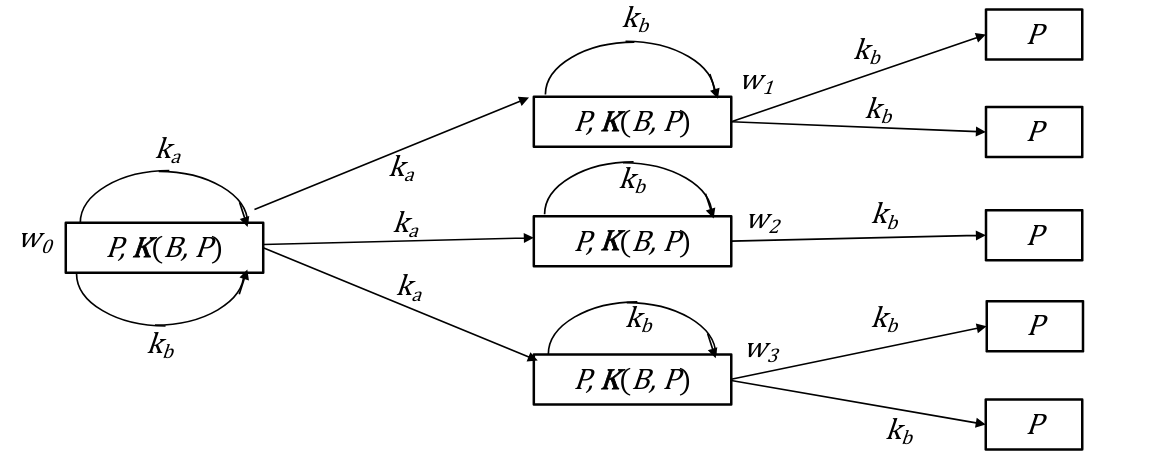
\includegraphics[width=\textwidth]{Images/nestedKnowledge}
    \caption{Example of Nested knowledge statements}
    \label{img:nestedKnowledge}
\end{figure}
Many of the properties that we desire for knowledge (and belief) can be achieved by
imposing constraints to the accessibility relation, so we define:
\begin{enumerate}
   \item Agents should be able to reason with the knowledge they have
         \[ K(a , \alpha \Rightarrow \beta) \Rightarrow (K(a, \alpha) \Rightarrow 
	    K(a, \beta)) \]
	 This is implicit in possible world semantics and is called 
	 \emph{Distribution axiom}.
   \item Agents cannot have false knowledge (different for beliefs)
         $K(a, \alpha) \Rightarrow  \alpha$ and this is called \emph{Knowledge axiom}.

	 The knowledge axiom is satisfied if the accessibility relation is reflexive and 
         this implies that there is at least a world accessible from $w$.

   \item It is also reasonable to assume that if an agent knows something, than it 
	 knows that it knows, that is formally
	 \[ K(a, \alpha) \Rightarrow K(a, K(a, \alpha)) \]
	 The accessibility relation must be transitive and this property is called
	 \emph{positive introspection}.
   \item In some axiomatization we also assume that if an agent doesn't know something,
         then it knows that it doesn't know it, that is formally
	 \[ \not K(a, \alpha) \Rightarrow K(a, \not K(a, \alpha)) \]
	The accessibility relation must be euclidean and this property is called
	\emph{Negative introspection}
   \item It is also intrinsic in possible world semantics that an agent knows all
	 the logical theorems, including the ones characterizing knowledge.\newline
         From $\vdash \alpha$ infer $K(a, \alpha)$ and this is 
	 \emph{Epistemic necessitation rule}.
   \item From 1 and 5, in the propositional case we also get rules
	 \[ \alpha \vdash \beta \land K(a, \alpha) \text{ we infer } K(a, \beta) \]
	 \[ \vdash \alpha \Rightarrow \beta \text{ we infer} 
	    K(a, \alpha) \Rightarrow K(a, \beta) \]
	 This is called \emph{Logical omniscience}, that is considered problematic,
	 since we are assuming unbounded reasoning capabilities.\newline
	As a corollary of logical omniscence we can infer $K$ distribution over and
	\[ K(a, \alpha \land \beta) \equiv K(a, \alpha) \land K(a, \beta) \]
\end{enumerate}

Modal epistemic logics are obtained with various combinations of axioms $1$-$4$ 
plus inference rule $5$, so we have System $K$ has only axiom $1$, system $T$ has 
axioms $1$-$2$, logic $S4$ has axioms $1$-$3$ and logic $S5$ has axioms $1$-$4$.\newline
Not any combination is possible since the properties of accessibility relations are
interdependent, so for example reflexive implies serial and if a relation is 
reflexive and Euclidian it is also transitive (axiom $2$ and $4$ imply $3$).

We have also consider the wise-men puzzle visible in figure \ref{img:wisemen}, where
we can also see an explanation of what consist.

\begin{figure}
	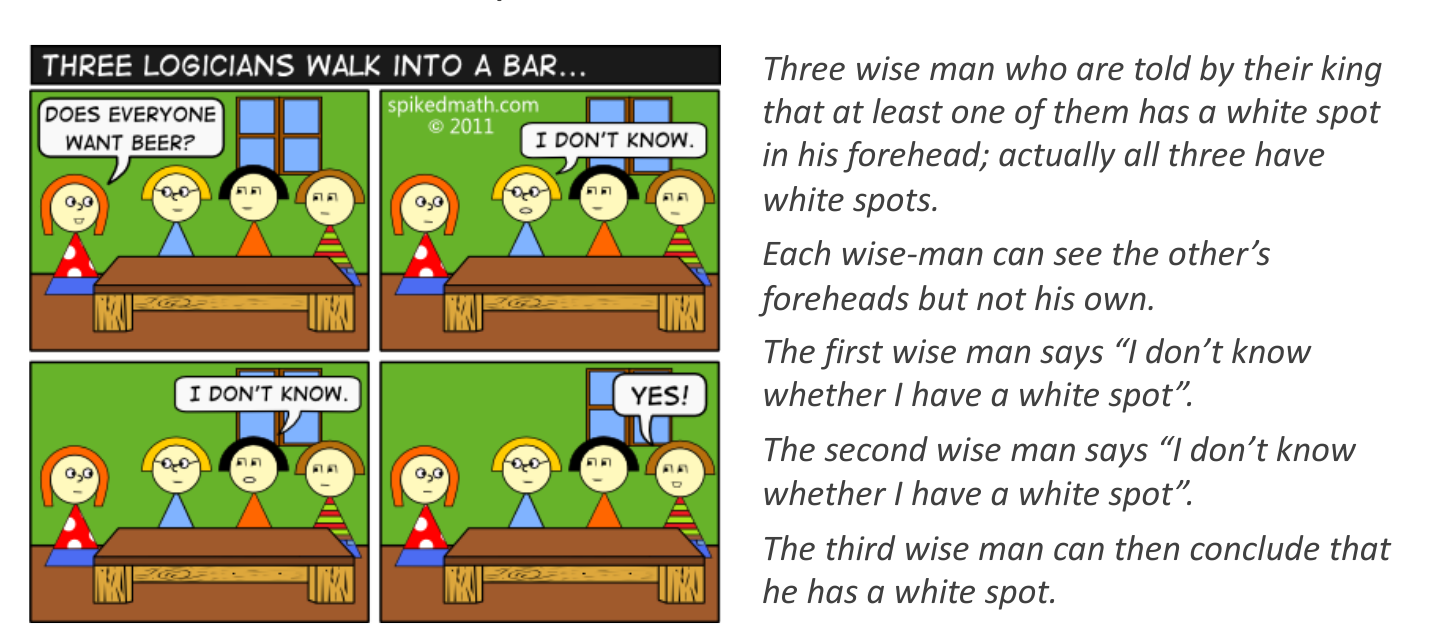
\includegraphics[width=0.8\textwidth]{Images/wiseman}
	\caption{Description of Wise-men puzzle}
	\label{img:wisemen}
\end{figure}
Since an agent can hold wrong beliefs the knowledge axiom is not appropriate, so 
we include as axiom the following instead
\[ \not B(a, False) \]
The distribution axiom and the necessitation rule are controversial, since an agent
cannot realistically believe all the logical consequences of its beliefs but
only those that he is able to derive (limited/bounded rationality), so 
\[ B(a, \alpha) \Rightarrow B(a, B(a, \alpha)) \]
\[ B(a, \alpha) \Rightarrow K(a, B(a, \alpha)) \]
Negative introspection is problematicm but with the following special case of
the knowledge axioms is safe $B(a, B(a, \alpha)) \Rightarrow B(a, \alpha)$

One disadvantage of default logic is that default rules are not sentences and
cannot be combined or reasoned about, so for example $\alpha: \beta / \gamma$
does not derive $\alpha: \beta / (\gamma \lor \delta)$.\newline
A different approach is to reason about defaults within a logic with a belief
operator $B$, where $B\alpha$ stands for "$\alpha$ is believed to be true”, and this
is \emph{autoepistemic logic}.\newline
The $B$ operator could be used to represent defaults, for example, as follows
\[ \forall x Bird(x) \land \not B \not Flies(x) \Rightarrow Flies(x) \]
Note that $B \not Flies(x)$ is different from $\not Flies(x)$

Given a KB that contains sentences using the B “auto-epistemic” operator, the 
minimal properties for a set of beliefs $E$ to be considered stable are the reasonable
set of beliefs to hold:
\begin{description}
 \item [Closure under entailment: ] if $E \models \alpha$, then $\alpha \in E$.
 \item [Positive introspection: ] if $\alpha \in E$, then $B \alpha \in E$.
 \item [Negative introspection: ] if $\alpha \not \in E$, then $\not B \alpha \in E$
\end{description}
This leads to the following definition of stable expansion of a KB
(a minimal set satisfying the properties yet described)
\begin{defi}[Stable expansion]
  A set $E$ is a stable expansion of $KB$ if and only if for every sentence $\phi$,
  it is the case that
  \[ \phi \in E \iff KB \cup \{B\alpha : \alpha \in E\} \cup 
                     \{\not B \alpha : \alpha \not \in E\} \models \phi \]
\end{defi}
The implicit beliefs $E$ are those sentences that are entailed by KB plus the 
assumptions deriving from positive and negative introspection.

The KB consisting of the sentence $(\not B p \Rightarrow p)$ has no stable expansion,
since if $B p$ is false, then the expansion entails $p$ and if $B p$ is true, then the
expansion does not include $p$.\newline
The KB consisting of the sentences $(\not B p \Rightarrow q)$ and $(\not B q \Rightarrow p)$
has exactly two stable expansions, so if $B p$ is true and $B q$ false the KB entails
$p$ and does not entail $q$, another stable expansion is when $B p$ is false and 
$B q$ is true.

\section{Reason Maintenance Systems}
Reason Maintenance Systems are the monotonic view of reasoning, so truth never changes,
the only allowed reasoning is to discover new truths.\newline
If the KB becomes inconsistent, there is not much you can do and common sense
reasoning requires belief revision mechanisms.\newline
We want to be able to make assumptions (defeasible reasoning) and if the world changes,
RETRACT is also an option (belief update).

RMS are practical systems designed to support beliefs revision, since they record
the reasons for believing something and do the job of maintaning consistency
in the belief set on behalf of the problem solver.

Many of the inferences drawn by a knowledge representation system will have only
default status or tentative nature and inevitably, some of these inferred facts
will have to be retracted; this process is called \emph{belief revision} and
can be problematic.\newline
One simple approach to belief revision is to number sentences according to the order
of assertion $P_1, P_2, \dots P_n$, so when the call $RETRACT(KB, P_i)$ is made, the 
system revert to the state just before $P_i$ was added, removing both $P_i$ and any
inferences derived from $P_i$.\newline
Sentences $P_{i+1}$ through $P_n$ can be added again if it is the case.

Reason Maintenance Systems (JTMS, ATMS), are reasoning mechanisms designed to handle
these problems efficiently and general architecture is visible in figure \ref{img:rms},
where the problem solver communicates facts, rules, assumptions along with their
justifications to the RMS and the PS may retract assertions, or may request to
handle inconsistencies.\newline
The RMS maintains beliefs, handles contradictions, restores consistency, performs
beliefs revision, generates explanations and provides the PS 
with an up-to-date set of beliefs.

\begin{figure}
	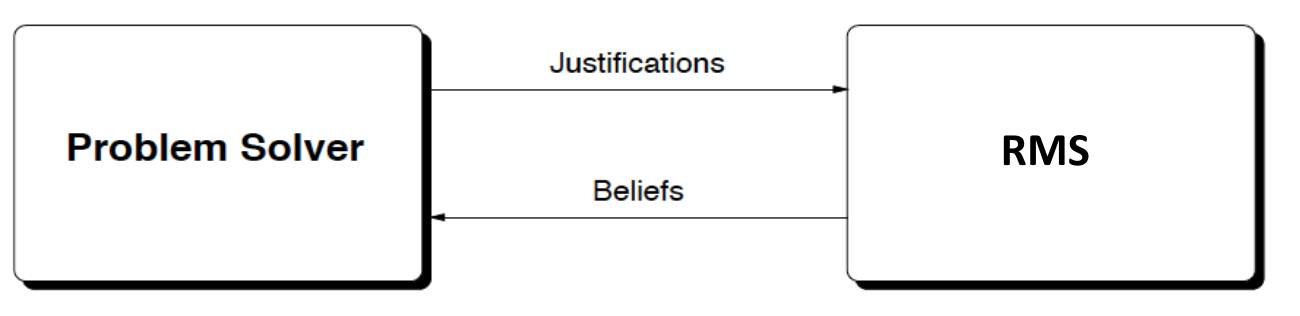
\includegraphics[width=\textwidth]{Images/architectureRMS}
	\caption{General Architecture of RMS}
	\label{img:rms}
\end{figure}
Rational thought is the process of finding reasons for attitudes, so has justified
belief or reasoned argument, rather than truth and the RMS handles a network of nodes
as propositional variables, representing propositions, rules and justifications.

Nodes are of different types: premises, assumptions, contradictions and have different
support according to the type of RMS and we will look at two of them:
\begin{itemize}
  \item JTMS (Justification-based Truth Maintenance Systems).
  \item ATMS (Assumption-based Truth Maintenance Systems)
\end{itemize}
In JTMS Each assertion in the knowledge base is represented as a node in the TMS with an
associated set of SL-justifications.\newline
Each SL-justification has two components:
\begin{description}
    \item [Inlist: ] the set of sentences from which it was inferred.
    \item [Outlist: ] a nonmonotonic justification the set of propositions that
	             should be false for the beliefs to be supported.
\end{description}
Examples:
\[ R (SL \{ \} \{ \}) \]
\[ Q (SL \{P, P \Rightarrow Q \}, \{\}) \]
\[ P (SL \{ \} \{\neg  P \}) \]
A node can have more than one SL justification (a justification set), since there
can be different reasons.

With JTMS, $RETRACT(KB, P)$ will delete exactly those sentences for which $P$ is a
member of every justification, so we have the following cases:
\begin{itemize}
 \item If a sentence $Q$ had the single justification $\{P, P \Rightarrow Q \}$, 
       then $Q$ would be removed.
 \item If it had the additional justification $\{P, P \lor R \Rightarrow Q \}$,
       then $Q$ would still be removed.
 \item If it also had the justification $\{R, P \lor R \Rightarrow Q \}$,
       then $Q$ would be maintained.
\end{itemize}
The JTMS, rather than deleting a sentence from the knowledge base
entirely when it loses all justifications, marks the sentence as being "out".\newline
If a subsequent assertion restores one of the justifications, then the
sentence is marked as "in" again, so we no need to re-compute inferences.

The node for proposition $P$ can be in one of two support states:
\begin{description}
 \item [IN: ] $P$ has at least one currently valid reason/justification,
	      and thus is a member of the current beliefs.
 \item [OUT: ] $P$ has no currently acceptable reason/justifications and
	       thus is not a member of the current beliefs.
\end{description}
A justification (SL inlist outlist) is valid iff each node in its inlist is IN,
and each node in its outlist is OUT and this creates a network of dependencies.\newline
Beliefs revision algorithms operate on these networks propagating effects and 
an example of that is visible in figure \ref{img:slList} and \ref{img:exSlList}.

\begin{figure}
	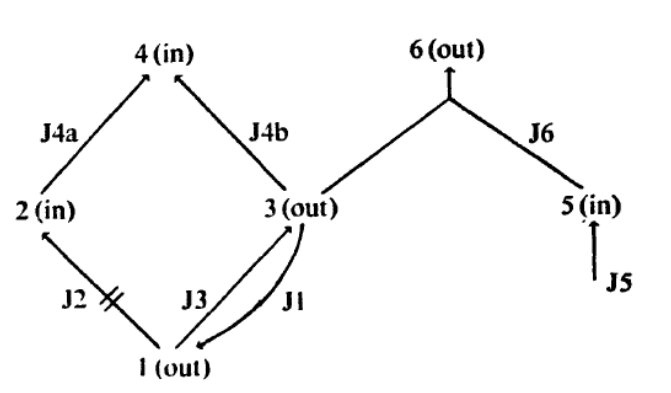
\includegraphics[width=\textwidth]{Images/slList}
	\caption{Example of SlList}
	\label{img:slList}
\end{figure}

\begin{figure}
	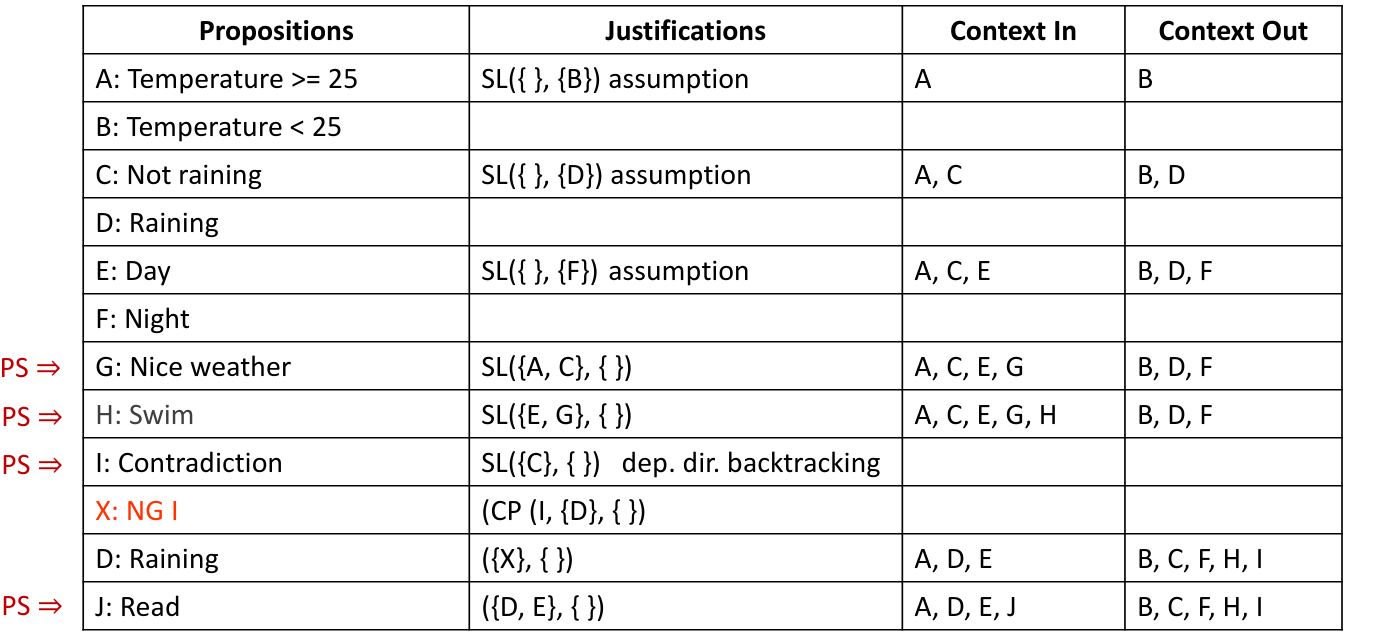
\includegraphics[width=\textwidth]{Images/exampleSlList}
	\caption{Complete example of Sllist in JTMS system}
	\label{img:exSlList}
\end{figure}

JTMSs can be used to speed up the analysis of multiple hypothetical situations, so
in a JTMS, the maintenance of justifications allows you to move quickly from one
state to another by making a few retractions and assertions, but at any time only
one contexts is represented.\newline
Taking the idea one step forward we could let multiple contexts to co-exist rather
than a global state of INs and OUT’s.

An Assumption based Truth Maintenance System (ATMS) represents all the contexts
been considered at the same time, so alternative contexts are explicitly stored.\newline
An ATMS-node is characterized by a label and justifications:
\begin{itemize}
 \item The label consists in a number of assumption sets (environments) and 
       the node holds when there is at least one supporting environment
       (with true assumptions).
 \item ATMS justifications are Horn formulas of the form $C :- L_1, L_2, \dots, L_n$,
       where $L_1, L_2, \dots, L_n$ are the antecendents and $C$ is the consequent of 
       justistification.
\end{itemize}
Thus a node is a triple $<n, E, J>$, where $n$ stands for an external sentence,
the description and in figure \ref{img:dependencyGraph} is possible to note an 
example of dependency graph.

\begin{figure}
	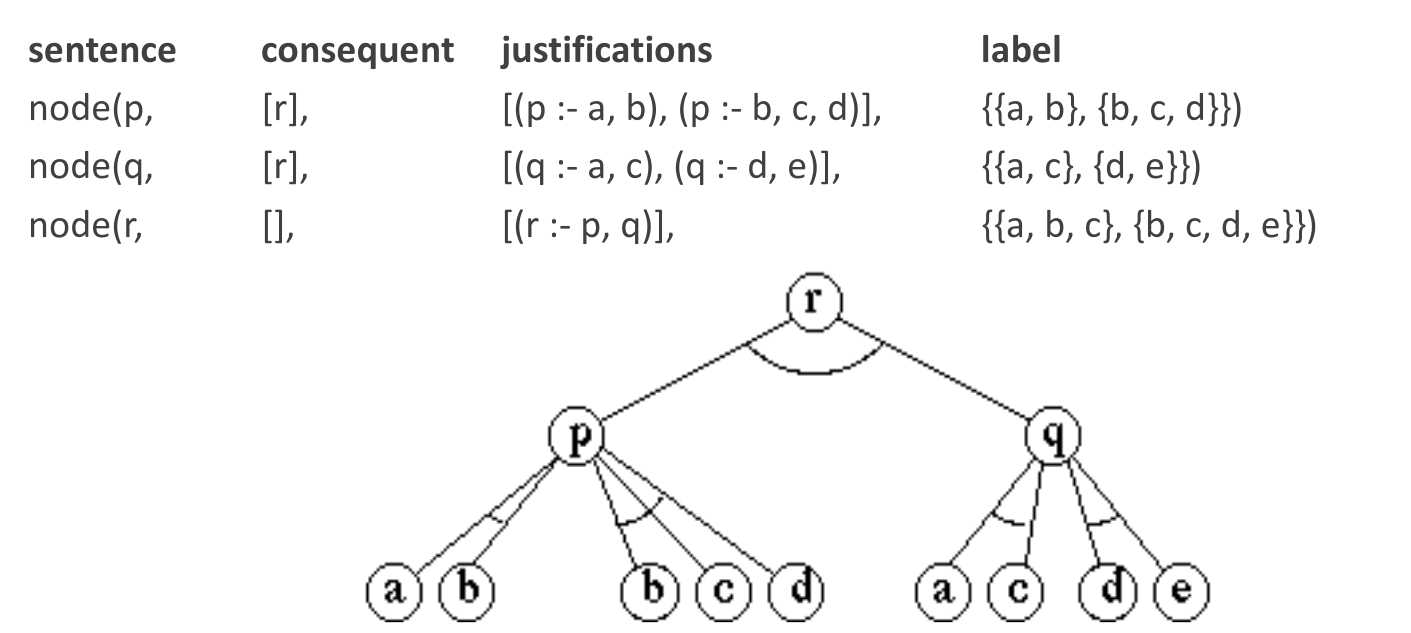
\includegraphics[width=\textwidth]{Images/dependencyGraph}
	\caption{Example of ATMS Dependency graph}
	\label{img:dependencyGraph}
\end{figure}

We have four types of nodes, according to the form of E and of J:
\begin{description}
 \item [Premise nodes: ] nodes always true, so the proposition can be believed
	                 without having to assume anything ($<n, \{\{ \}\}, \{( )\}>$.
 \item [Assumption nodes: ] these nodes are justified by themselves $<n, \{(n)\},\{(n)\}>$
 \item [Derived nodes: ] Maintain the set of assumptions made and the justifications.
 \item [Contradictions: ] an environment can be inconsistent when its assumptions are
	 contradictory, therefore must be removed, and these environments
	 are called \emph{nogoods}.
\end{description}
The fundamental operation is updating environments and deciding whether a
proposition holds in a given environment, so a node $n$ holds in a given 
environment $E$, iff it can be derived from $E$ given 
the set of justifications $J: E, J \vdash n$.

ATMS allow for quick generation of explanations, so an explanation of a sentence
$P$ is a set of sentences $E$ such that $E \models P$, usually a minimal
one is preferred and explanations can be assumptions.\newline
ATMS can generate explanations by making tentative assumptions and looking if the
label for the sentence  "car won’t start" contains the assumptions
that would justify the sentence.

\section{Semantic Networks and Frames}
We have that the logical approach is suitable to model rational reasoning, instead 
the cognitive–linguistic approach is more concerned with understanding the mechanisms
for knowledge acquisition, representation and use of knowledge in human minds and 
has synergies with other fields, such as cognitive psychology and linguistics.

In logic systems, symbolic expressions are modular and are syntactically transformed
without paying attention to the symbols used or to their “meaning”, infact 
the symbol themselves are arbitrary and it is all a matter of writing axioms 
to restrict interpretations.\newline
Associationist theories are instead concerned with the connections among symbols and
the meaning that emerges from these connections.\newline
The idea is that meaning of a word emerges as a result of the connections to other words
and connections are shaped by experience, as for example from reading texts.

The question is how the meaning of words is acquired, represented and used, and we have that
the memory itself is distinguished in:
\begin{description}
   \item [Episodic memory: ] specific facts and events.
   \item [Semantic memory: ] abstract and general knowledge.
\end{description}
Semantic networks is a graphical model proposed for semantic memory and we 
represent two kinds of knowledge:
\begin{description}
   \item [Concepts: ] the semantic counterpart of words, represented as nodes.
   \item [Propositions: ] relations among concepts, represented as labelled arcs.
\end{description}
It is not accounting for dynamic aspects of memory and learning and there are other models
like \emph{Distributional models}, like word embeddings,
or connectionist models for learning.

\begin{figure}
	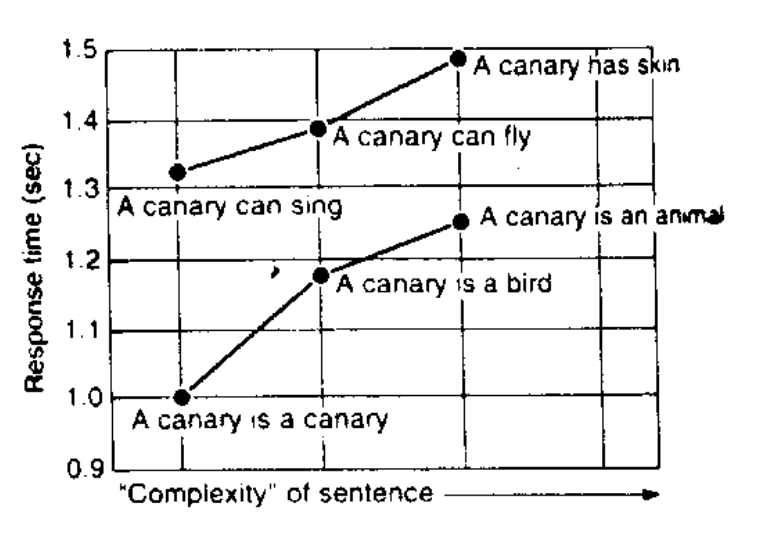
\includegraphics[width=\textwidth]{Images/cognitive}
	\caption{Example of a cognitive psychology definition}
	\label{img:cognitive}
\end{figure}

Cognitive psychology is an experimental discipline and
we have an example in figure \ref{img:cognitive}.\newline
Evidence are for hierarchical organization, properties are attached to the most general
concept to which they apply and exceptions are attached directly to the objects, like 
as possible to note in figure \ref{img:hierarchical}.\newline
Success of hierarchical organization of concepts in computer science and
influence on OOP languages in SW engineering.

\begin{figure}
	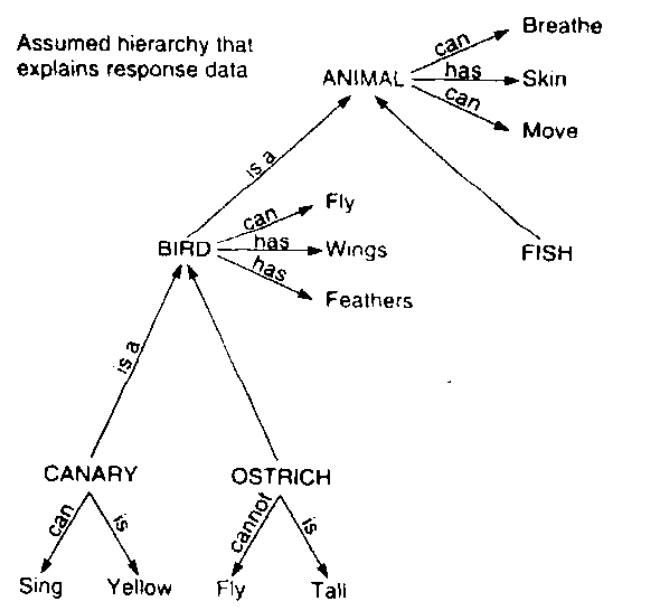
\includegraphics[width=\textwidth]{Images/hierarchical}
	\caption{Example of Hierarchical organization}
	\label{img:hierarchical}
\end{figure}

Semantic networks are a large family of graphical representation schemes and 
a semantic network is a graph where nodes, with a label, correspond to concepts
and arcs, labelled and directed, correspond to binary relations
between concepts, often called roles.\newline
Nodes come in two flavors:
\begin{description}
   \item [Generic concepts] corresponding to categories/classes
   \item [Individual concepts], corresponding to individuals
\end{description}
Two special relations are always present, with different names:
\begin{description}
    \item [IS-A: ]    holds between two generic concepts (subclass).
    \item [Inst-Of: ] holds between an individual concept and a class (member of).
\end{description}
Inheritance is very conveniently implemented as link traversal, as we can see in figure 
\ref{img:inheritance}, and Multiple inheritance is also allowed, but is banned in OOP.

\begin{figure}
	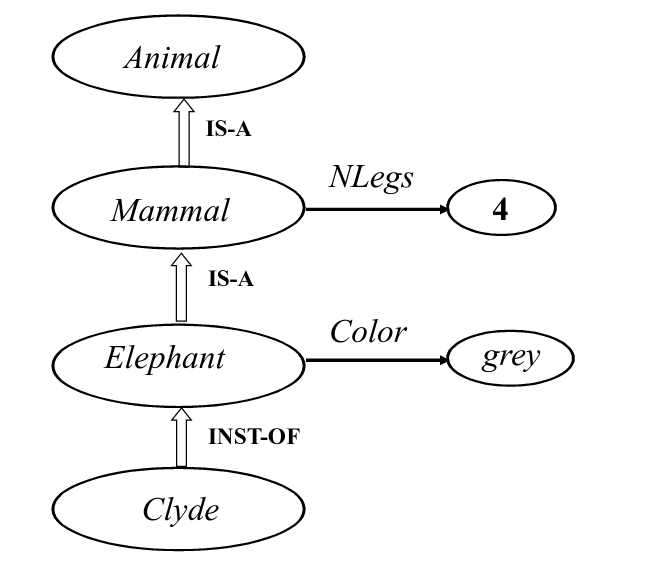
\includegraphics[width=\textwidth]{Images/inheritanceExample}
	\caption{Example of Inheritance in Semantic Network}
	\label{img:inheritance}
\end{figure}
The presence of exceptions does not create any problem, so we just take the most
specific information: the first that is found going up the hierarchy.\newline
Even if they can express n-ary predicates, semantic networks do not have the same
expressive power of FOL:
§ Existentials, $\lor$ and $\Rightarrow$ are not expressible or are expressible
only in special cases and this is not necessarily a bad thing since it suggests
a subset of FOL with interesting computational properties, explored in description logics.

A well -known example in AI are Sowa’s conceptual graphs, inspired by Pierce’s
existential graphs and they candidate as an intermediate schema for representing
natural language.\newline
Conceptual graphs, visible in figure \ref{img:conceptual}, rectangles are concepts
(possibly typed as in Person: John), circles are called conceptual relations:
the label is the name of the relation.

\begin{figure}
	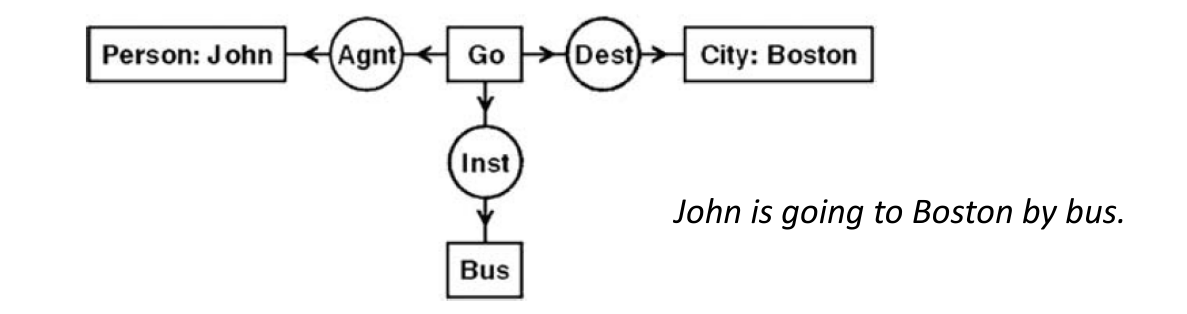
\includegraphics[width=\textwidth]{Images/conceptualGraph}
	\caption{Example of Conceptual graph}
	\label{img:conceptual}
\end{figure}

A more complex proposition, including implication, uses context boxes, so for example
“If a farmer owns a donkey, then he beats it” is represented in figure \ref{img:context}.

\begin{figure}
	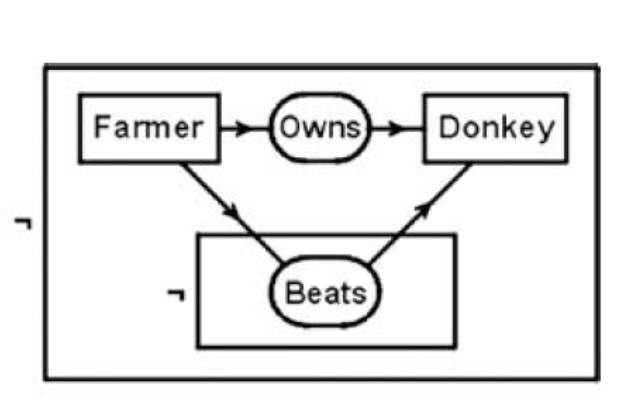
\includegraphics[width=\textwidth]{Images/complexConceptual}
	\caption{Complex example of Conceptual graph}
	\label{img:context}
\end{figure}
Woods and others point out the lack of “semantics” of semantic nets, so as a result
in the $80$’s KL-One introduces important ideas:
\begin{itemize}
   \item Concepts and roles (they are also nodes with a different status).
   \item Value restrictions ($v/r$)
   \item Numerical restrictions ($1$, NIL)
   \item A formal semantics
\end{itemize}
The double arrow is a IS-A relation and an example in figure \ref{img:klOne}.

\begin{figure}
	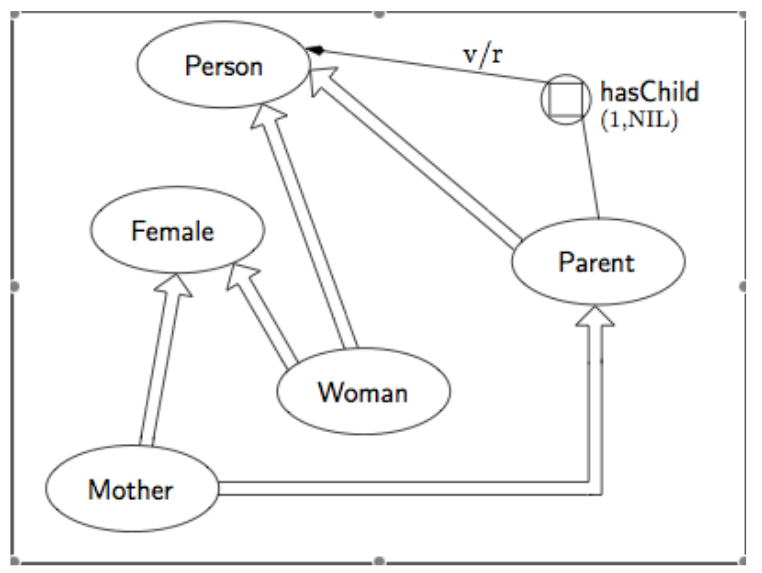
\includegraphics[width=\textwidth]{Images/klOne}
	\caption{Example of IS-A relation in KL One}
	\label{img:klOne}
\end{figure}
We may look at semantic networks as a convenient implementation for a part of
FOL and a representation and mechanism at the symbol level 
rather than at the knowledge level, with concepts defined in figure \ref{img:knowledgeConc}.

\begin{figure}
	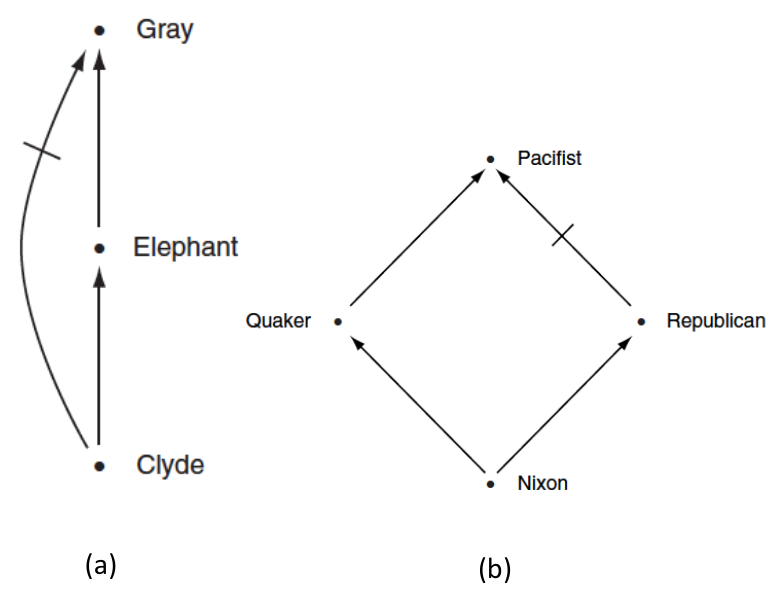
\includegraphics[width=\textwidth]{Images/knowledgeConc}
	\caption{Definition of representation done at the symbol level}
	\label{img:knowledgeConc}
\end{figure}
A more essential notation for inheritance networks are negated arcs, so more specific
information should win and there is also multiple inheritance, as we can see in figure
\ref{img:inheritanceNetwork}.

\begin{figure}
	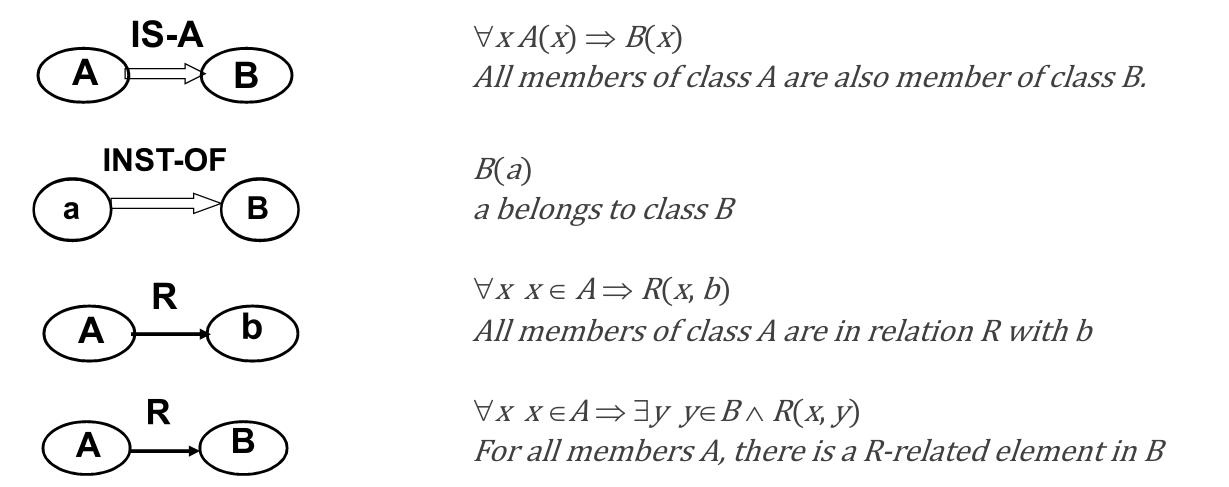
\includegraphics[width=\textwidth]{Images/inheritanceNetwork}
	\caption{Example of Inheritance Network}
	\label{img:inheritanceNetwork}
\end{figure}
Not so easy and there are two strategies:
\begin{itemize}
    \item Shortest path heuristics, based on minimal path length.
    \item Inferential distance, based on the topology (not path length).
\end{itemize}
The shortest path strategy fails in presence of redundant links such as $q$ (shortcuts),
as we can see in figure \ref{img:shortest} and the inferential distance strategy:
$A$ closer to $B$ than $C$ iff there is a path from a $A$ to $C$ through $B$.\newline
With shortest path it would conclude that Clyde is grey, instead inferential distance
it would conclude that Clyde is not grey.

\begin{figure}
	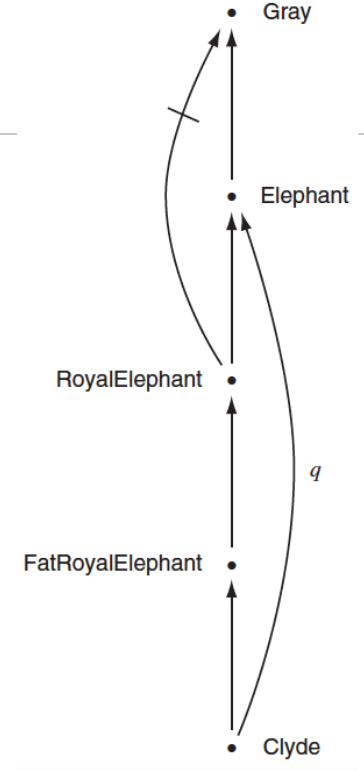
\includegraphics[width=\textwidth]{Images/shortestError}
	\caption{Example of shortest path failure with redundant links}
	\label{img:shortest}
\end{figure}

\emph{WordNet}, a big lexical resource organized as a Semantic network ($122.000$ terms),
names, verbs, adjectives, adverbs are organized in sets of synonims (synsets) which
are a representation of a concepts ($117.000$ synset); a syntactic word is associated
with a set of synsets: the word senses and uses of WordNet in computational linguistics are:
\begin{itemize} 
   \item Query expansion with synonyms or hyperonyms.
   \item Semantics distance among words.
   \item Word sense disambiguation.
   \item Semantic category of a word (or supersense).
\end{itemize}
The structure of WordNet is visible in figure \ref{img:wordnet}.

\begin{figure}
	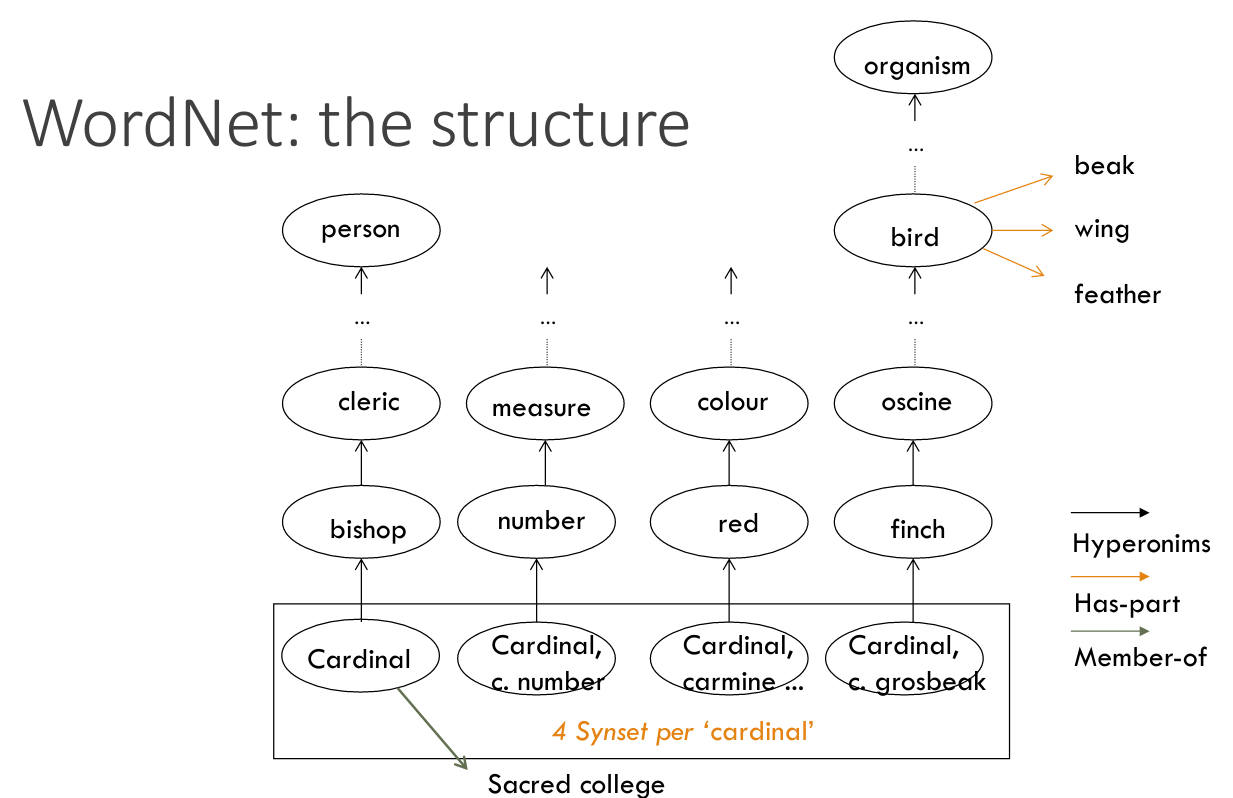
\includegraphics[width=\textwidth]{Images/wordnet}
	\caption{Structure of WordNet}
	\label{img:wordnet}
\end{figure}
\emph{Knowledge graphs} are large-scale knowledge bases have been built including:
\begin{description}
    \item [Open access: ] Dbpedia, WikiData, Freebase, YAGO.
    \item [Proprietary: ] Microsoft's Satori, Google's Knowledge Graph,
	                  Google’s Knowledge vault.
\end{description}
From $2012$ Google uses the knowledge graph with its search engine, structured data
coming from many sources, including the CIA World Factbook, Wikidata, Wikipedia, Freebase
and has more than $70$ billion facts in $2016$.\newline
Since $2014$, Google’s Knowledge Vault contains facts derived automatically from the
web with machine learning techniques and facts have an associated confidence value.

It is very natural to think of knowledge not as a flat collection of sentences, but
rather as structured and organized in terms of the objects the knowledge is about.\newline
Complex objects have attributes, parts constrained in various ways, objects might have
a behavior that is better expressed as procedures and this is very much
as in Object Oriented Programming.\newline
Marvin Minsky in $1975$ suggested the idea of using a structured representation
of objects, called frames, to recognize and deal with new situations.

Knowledge is organized in complex mental structures called \emph{frames}, and 
the essence of the theory is "When one encounters a new situation (or makes a 
substantial change in one's view of the present problem) one selects from memory
a structure called a frame.\newline
This is a remembered framework to be adapted to fit reality 
by changing details as necessary.".\newline
A frame is a data-structure for representing a stereotypical object or situation.

There are two types of frames:
\begin{description}
   \item [individual frames] used to represent single objects.
   \item [generic frames] used to represent categories or classes of objects.
\end{description}
An individual frame is a collection of slot-fillers pairs, and fillers can be:
\begin{itemize}
   \item values, usually default values.
   \item constraints on values.
   \item the names of other individual frames.
   \item the special slot INSTANCE-OF
\end{itemize}
Generic frames are similar and fillers can be the special slot IS-A or procedures 
like IF-ADDED, activated when the slot receives a value and IF-NEEDED,
activated when the value is requested.\newline
These procedures are called procedural attachments or demons, so the :INSTANCE-OF 
and :IS-A slots organize frames in frame systems.\newline
They have the special role of activating inheritance of properties and procedures.\newline
In frames, all values are understood as default values, which can be overridden and
example of frames are visible in figure \ref{img:frames}.\newline
Attached procedures provide a flexible, organized framework for computation and 
reasoning has a procedural flavor.\newline
A basic reasoning loop in a frame system has three steps:
\begin{description}
   \item [Recognition: ] a new object or situation is recognized as instance
	                 of a generic frame.
   \item [Inheritance: ] any slot fillers that are not provided explicitly but can be 
	                 inherited by the new frame instance are inherited.
   \item [Demons: ] for each slot with a filler, any inherited IF-ADDED procedure is run,
       possibly causing new slots to be filled, or new frames to be instantiated,
       until the system stabilizes, then the cycle repeats.
\end{description}
\begin{figure}
	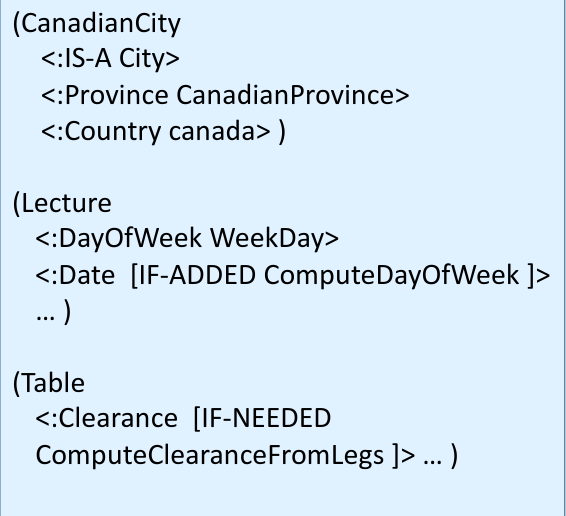
\includegraphics[width=\textwidth]{Images/frames}
	\caption{Example of Frames}
	\label{img:frames}
\end{figure}
When the filler of a slot is requested:
\begin{enumerate}
    \item if there is a value stored in the slot, the value is returned.
    \item otherwise, any inherited IF-NEEDED procedure is run to compute the filler
	  for the slot, and this may cause other slots to be filled, or new frames
	  to be instantiated.
\end{enumerate}
Frame-based representation languages and OOP systems were developed at the
same time, and they look similar and certainly one could implement 
a frame system with OOP.\newline
Important difference is that frame systems tend to work in a cycle:
\begin{itemize}
    \item Instantiate a frame and declare some slot fillers
    \item inherit values from more general frames
    \item trigger appropriate forward-chaining procedures
    \item when the system is quiescent, stop and wait for the next input
\end{itemize}
The designer can control the amount of "forward" reasoning that should be
done (in a data-directed fashion) or "backward" (in a goal-directed fashion).

Applications of frames are story understanding, Scene recognition in vision, tools
for building expert systems (possibly together with rules) and the idea of frames
was also used in building "FrameNet": a large NL resource based on the theory
of "frame-based" semantics.

\emph{FrameNet} is a resource consisting of collections of NL sentences syntactically and
semantically annotated, organized in frames.\newline
Frame semantics, the meaning of words emerges from the role they have in the 
conceptual structure of sentences and knowledge is structures in $16$ general domains:
time, space, communications, cognition, health and also has $6000$ Lexical elements,
and $130.000$ annotated sentences; 
an example in FrameNet is visible in figure \ref{img:framenet}.

\begin{figure}
	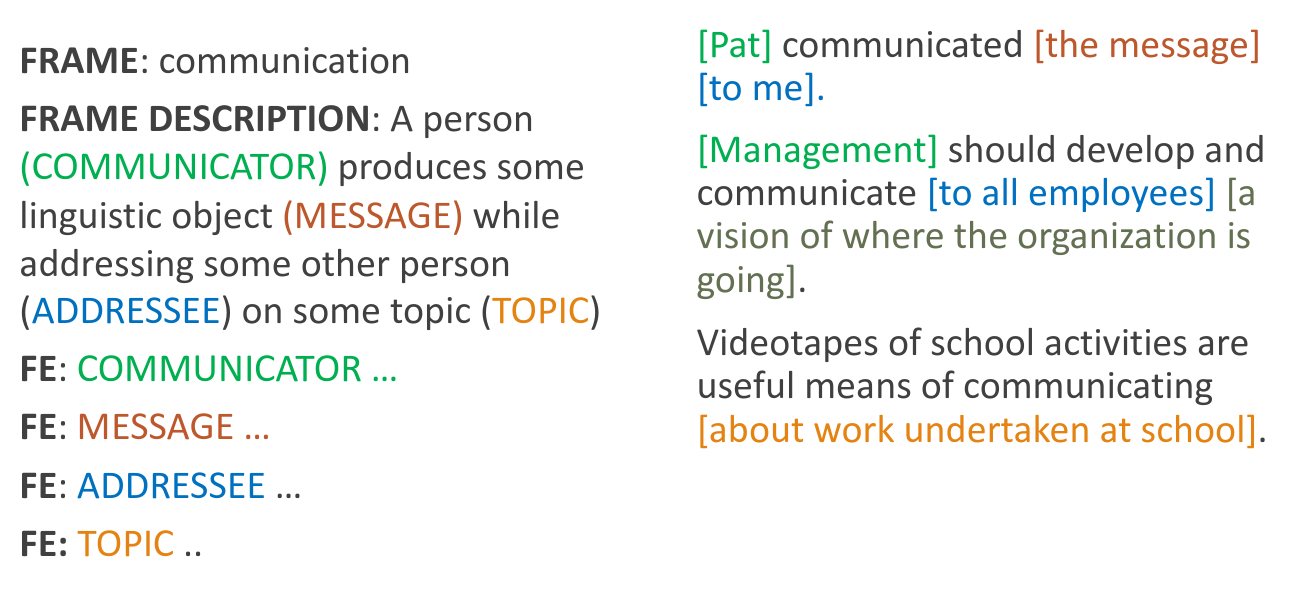
\includegraphics[width=\textwidth]{Images/framenet}
	\caption{Example of FrameNet}
	\label{img:framenet}
\end{figure}

\section{Description Logics}
Most of the reasoning takes place at the level of categories rather than on individuals,
so if we organize knowledge in categories and subcategories (in a hierarchy) it is enough
to classify an object, according to its perceived properties, in order to infer 
properties of the categories to which it belongs.\newline
Inheritance is a common form of inference, which exploits structure and also 
ontologies will play a crucial role, providing a source of shared and precisely defined
terms that can be used in meta-data of digital objects and real world objects.

In the $80$'s we assist to a formalization of the ideas coming from semantic
networks and frames resulting in specialized logics.\newline
These logics, called terminological logics and later description logics find an
important application in describing “domain ontologies” and represent the
theoretical foundations for adding reasoning capabilities to the Semantic web.\newline
\emph{Ontology} is a formal model of an application domain (a conceptualization) and
subclass relations are important in defining the terminology and serve to
organize knowledge in hierarchical taxonomies (shared ontologies are the basis
for the semantic web).

The \emph{Semantic Web} is the vision of Tim Berners-Lee ($1998$) to gradually
develop alongside the “syntactic web” (or web of documents), for communication among people,
a “semantic web” (or web of data) for communication among machines.\newline
The semantic web is a huge distributed network of linked data which can be used by programs
as well, provided their semantics is shared and made clear 
(this is the role of formal ontologies).\newline
These data comply with standard web technologies: Unicode encoding, XML, URI,
HTTP web protocol.

The technologies used in Semantic Web, visible in \ref{img:semantic}, are the following:
\begin{itemize}
   \item Unicode and URI (Universal Resource Identifier)
   \item XML for syntactic interoperability
   \item RDF (Resource Description Framework) is a language to describe binary
         relations between resources (subject, predicate, object).
   \item RDF schema (RDFS) used to define classes, relations between classes,
	 to constrain domains and co-domains of relations and this is basic language
	 for ontologies.
   \item OWL is the web ontology language, one among many description logics
         elected as standard by the W3C.
\end{itemize}
\begin{figure}
	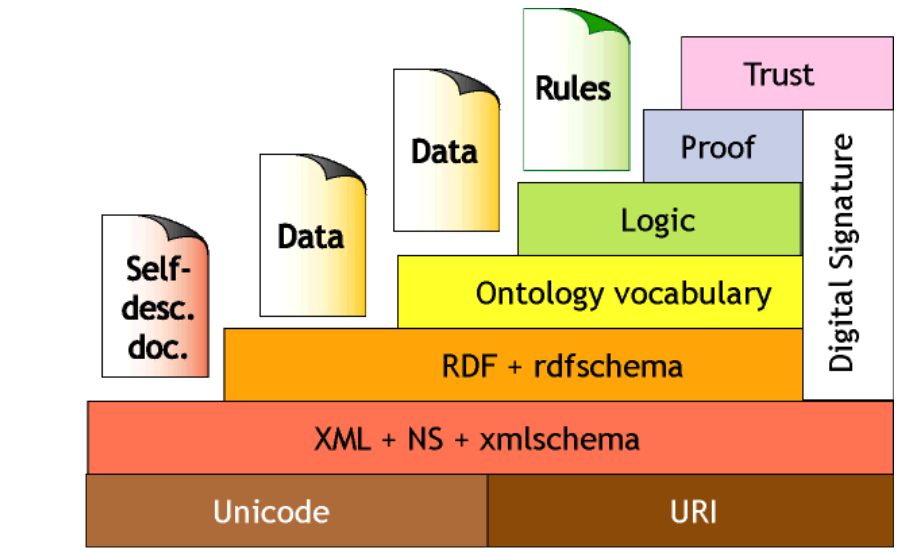
\includegraphics[width=\textwidth]{Images/semanticTechnologies}
	\caption{Technologies used in Semantic Web}
	\label{img:semantic}
\end{figure}
\emph{Description logics} can be be seen as:
\begin{enumerate}
   \item Logical counterparts of network knowledge representation schema, frames
         and semantic networks; in this formalization effort, defaults and exceptions
	 are abandoned and the ideas and terminology (concept, roles, inheritance
	 hierarchies) are very similar (to KLOne in particular).
   \item Contractions of first order logic (FOL), investigated to obtain better
         computational properties and attention to computational complexity/decidability
	 of the inference mechanisms.
\end{enumerate}
Each DL is characterized by operators for the construction of terms, that are of $3$ types:
\begin{description}
    \item [Concepts: ] corresponding to unary relations, with operators for the construction
	   of complex concepts: and($\cap$), or($\cup$), not($\neg$), all($\forall$), 
	   some ($\exists$), atleast ($\geq n$), almost ($\leq n$) and so on.
    \item [Roles: ] corresponding to binary relations, possibly together with operators
	            for construction of complex roles.
    \item [Individuals:]  only used in assertions.
\end{description}
Assertions are kept separate and can be only of two types:
\begin{itemize}
   \item $i: C$, where $i$ an individual and $C$ is a concept.
   \item $(i, j): R$, where $i$ and $j$ are individual and $R$ is a role.
\end{itemize}
In figure \ref{img:kbDescription} is possible to note an example of KB based on 
description logic and we define the logic $AL$ as the syntax of terms 
in figure \ref{img:logicAL}.

\begin{figure}
	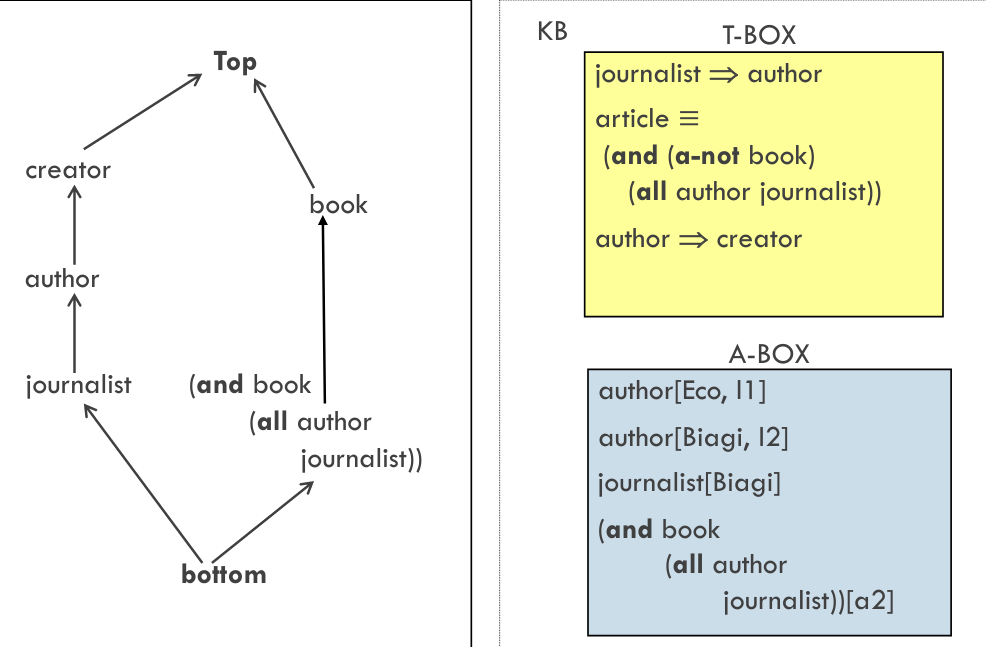
\includegraphics[width=\textwidth]{Images/exampleKB}
	\caption{Example of KB Description}
	\label{img:kbDescription}
\end{figure}
\begin{figure}
	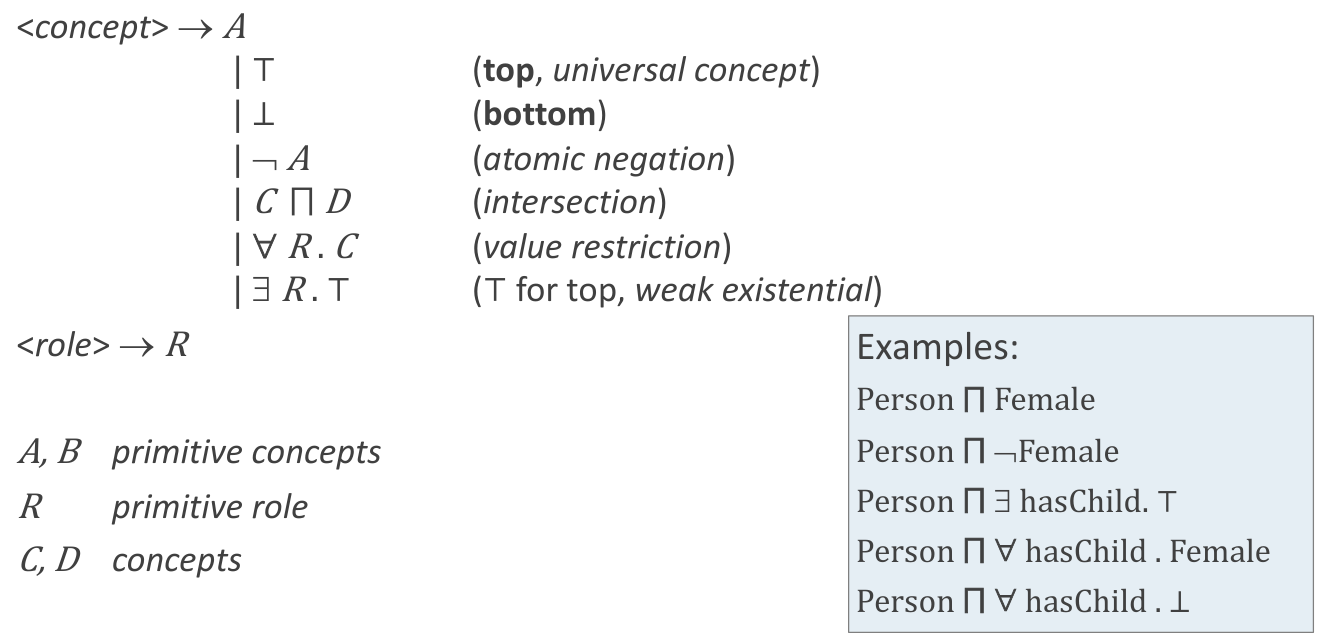
\includegraphics[width=\textwidth]{Images/logicAL}
	\caption{Definition of syntax of Logic $AL$}
	\label{img:logicAL}
\end{figure}
The semantics of $AL$ consist of $\Delta^I$, interpretation domain (a set of individuals) 
and $I$ an interpretation function which assign for atomic concepts 
$A: A^I \subseteq \Delta^I$, for atomic roles $R: R^I \subseteq \Delta^I \times \Delta^I$
and for individual constants $a: a^I \in \Delta^I$.\newline
We have some rules visible in figure \ref{img:semanticAL} and we have also $4$ 
more expressive logics, defined as:
\begin{description}
   \item [$U$ union: ] $(C \cup D)^I = (C^I \cup D^I)$ 
   \item [$E$ full existential: ] ($\exists R.C)^I = \{ a \in \Delta^I : \exists b. (a, b)
	                          \in R^I \cap b \in C^I \}$
   \item [$N$ numerical restrictions: ] 
	   \[ (\geq n R)^I = \{ a \in \Delta^I : |\{b : (a, b) \in R^I\}| \geq n\} \]
	   \[ (\leq n R)^I = \{ a \in \Delta^I : |\{b : (a, b) \in R^I\}| \leq n\} \]
   \item [$C$ full complement: ] $(\not C)^I = \Delta ^ I - C^I$
\end{description}
\begin{figure}
	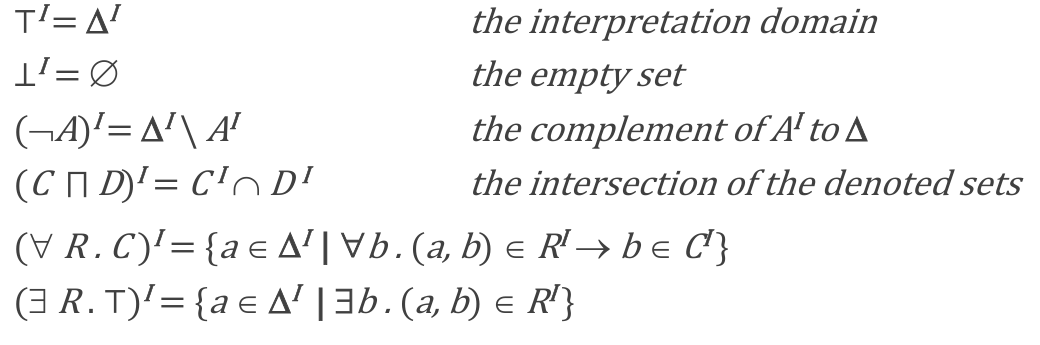
\includegraphics[width=\textwidth]{Images/rulesAL}
	\caption{Some rules for logic $AL$}
	\label{img:semanticAL}
\end{figure}
Different description logics are obtained by adding other constructors to AL and 
we obtain the lattice visible in figure \ref{img:ALLattice}, where not all of them 
are distinct so for example $ALUE = ALC$.

\begin{figure}
	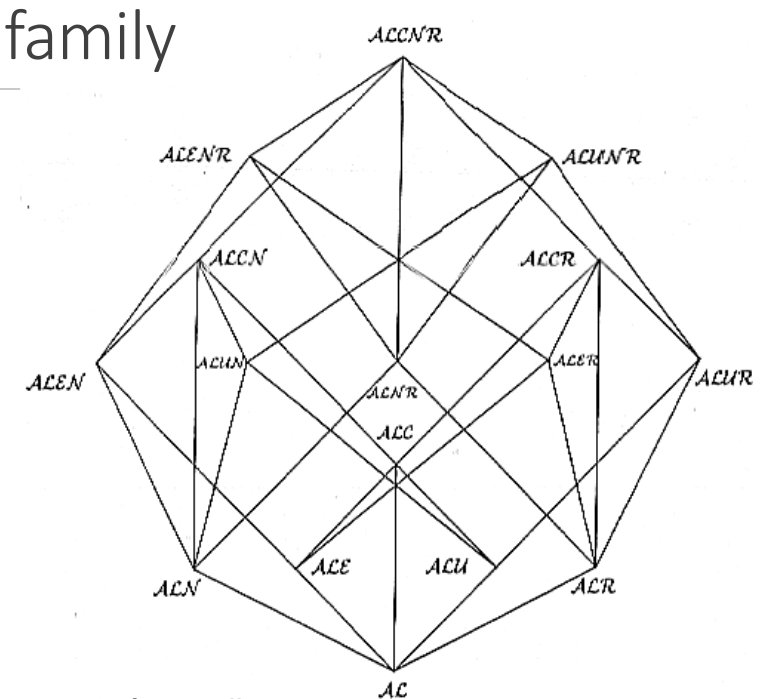
\includegraphics[width=\textwidth]{Images/ALLattice}
	\caption{Lattice of $AL$ logics}
	\label{img:ALLattice}
\end{figure}
We have the terminological axioms $T$ defined as:
\[ C \subseteq D \text{ inclusion of concepts } C^I \subseteq D^I \]
\[ R \subseteq S \text{ inclusion of roles } R^I \subseteq S^I \]
\[ C \equiv D \text{ equality of concepts } C^I \equiv D^I \]
\[ R \equiv S \text{ equality of roles } R^I \equiv S^I \]
We have that equalities introduce a symbol on the left and we have a \emph{terminology},
when symbols appear on the left not more than once; we have a \emph{primitive symbols} in
case appear only on the right and a \emph{defined symbols} if appear also on the left.

If a terminology is acyclic, an example is visible in figure \ref{img:acyclicTerm}, it can
be expanded by substituting to defined symbols their definitions.\newline
In the case of acyclic terminologies the process converges and the expansion $T^e$ is unique.

\begin{figure}
	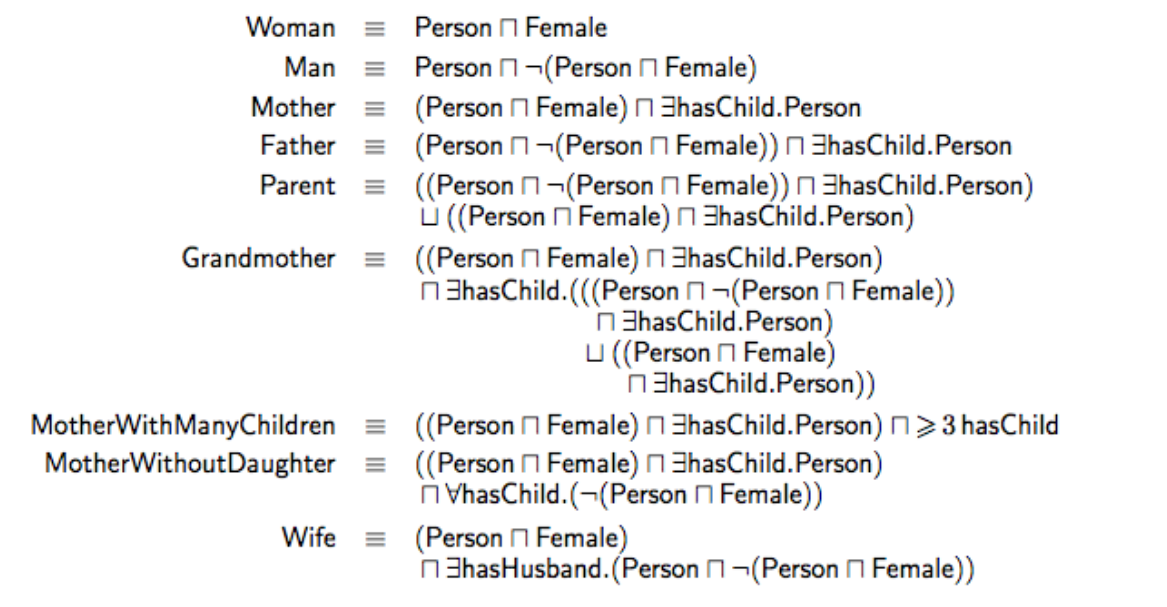
\includegraphics[width=\textwidth]{Images/acyclic}
	\caption{Example of Acyclic description logics}
	\label{img:acyclicTerm}
\end{figure}
Properties of $T^e$ are the following:
\begin{itemize}
   \item In $T^e$ each equality has the form $C \equiv D^e$ where $D^e$ contains only 
	 primitive symbols.
   \item $T^e$ contains the same primitive and defined symbols of $T$
   \item $T^e$ is equivalent to $T$.
\end{itemize}
An example of expansion is visible in figure \ref{img:expandedTerminology} and inclusion
axioms are called \emph{specializations}, like for example $Woman \subseteq Person$.\newline
A \emph{generalized terminolohy}, with inclusion axioms, if acyclic, can be transformed in 
an equivalent terminology with just equivalence axioms
\[ A \subseteq C \to A \equiv A' \cap C \]
where $A'$ is a new primitive symbol.\newline
This also means that specializations do not add expressive power to the language, 
at least in the case of acyclic terminologies.

\begin{figure}
	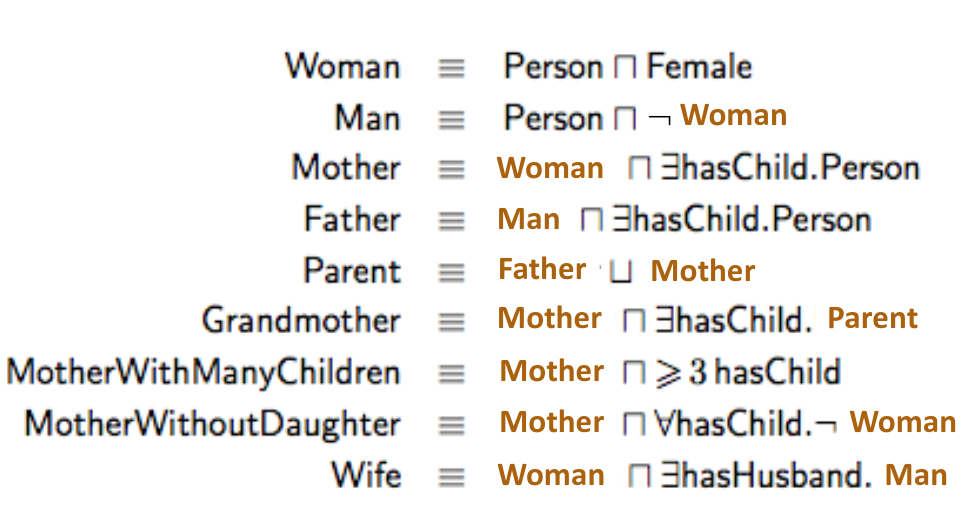
\includegraphics[width=\textwidth]{Images/expanded}
	\caption{Example of an expansion of terminology}
	\label{img:expandedTerminology}
\end{figure}
An A-BOX is a set of assertions of the following type $a: C$ assertion over concepts
(meaning $a^I \in C^I$) and $(b, c) : R$ assertions over roles (meaning $(b^I, c^I) \in R^I$,
where $a, b, c, d, \dots$ are individuals.\newline
In description logic we make an assumption that different indivudal constants refer to
different individuals, and that is called \emph{Unique Name Assumption} (UNA).

It is always possible to translate DL assertions into FOL, so we define a translation
function $t(C, x)$ which returns a FOL formula with $x$ free
\[ t(C, x) \to C(x) \]
In figure \ref{img:assertTranslation} we have translation rules for assertions and 
in figure \ref{img:termTranslatin} we have translation rules for terms.

\begin{figure}
	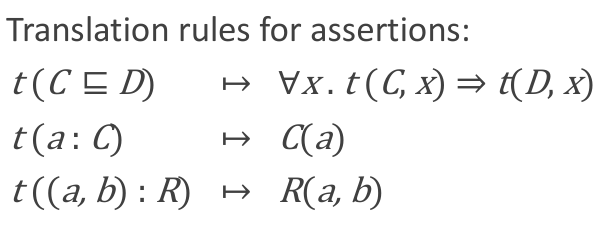
\includegraphics[width=\textwidth]{Images/assertTranslation}
	\caption{Translation rules for assertions}
	\label{img:assertTranslation}
\end{figure}

\begin{figure}
	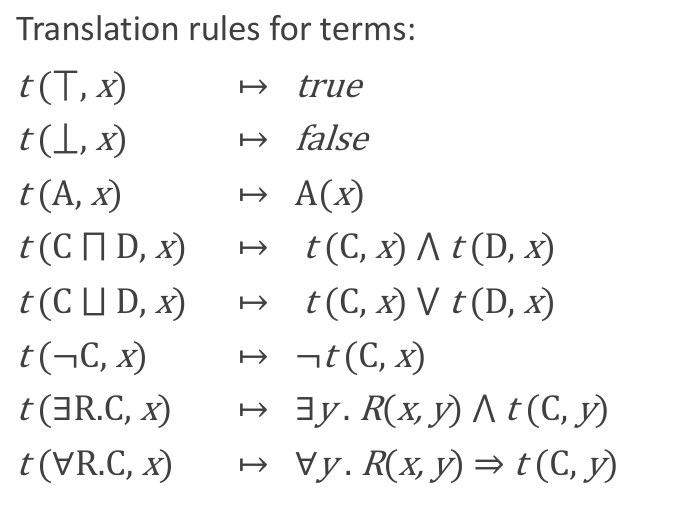
\includegraphics[width=\textwidth]{Images/termTranslation}
	\caption{Translation rules for terms}
	\label{img:termTranslatin}
\end{figure}
We have that the knowledge base in description logics is defined by $K = (T, A)$, where
$T$ is the T-BOX terminological component and $A$ is the A-BOX the assertional component.

An interpretation $I$ satisfies $A$ and $T$ (therefore $K$) iff it satisfies 
any assertion in $A$ and definition in $T$ ($I$ is a model of $K$).\newline

Classical decision problems in DL are the following:
\begin{description}
   \item [Satisfiability of a KB:]  $KBS(K)$ answer if there is a model for $K = (T, A)$.
   \item [Logical consequence of a KB: ] $K \models a:C$ also called instance checking.
   \item [Concept satisfiability $CS(c)$:] estabilish if is there an interpretation
	   different from the empty set.
   \item [Subsumption: ] $K \models C \subseteq D$ if for every model $I$ di $T$,
	   $C^I \subseteq D^I$.
   \item [Concept equivalence:] $K \models C \equiv D$.
   \item [Disjointness: ] answer if $C^I \cap D^I = \emptyset$ for any model $I$ of $T$.
   \item [Retrieval: ] find all individuals which are instances of $C$.
   \item [Most Specific Concept (MSC): ] given a set of individuals, find the most
	  specific concept of which they are instances and this is used for classification.
   \item [Least Common Subsumer (LCS): ] given a set of concepts, find the most specific
	 concept which subsumes all of them and is also used for classification.
\end{description}
Decision problems are not independent, infact all problems can be reduced to $KB$ 
satisfiability, so we have for esample that concept consistency is satisfied iff 
$K \cup \{a:C\}$ is satisfiable, instance checking $K \models a:C$ iff $K \cup \{a:\neg C\}$
is unsatisfiable; this is for some aspect reconduble to classic logic deduction.

The most used method is a technique for verifying satisfiability of a KB (KBS), and it is
a variant of a method for natural deduction, called \emph{semantic tableaux}
(It applies constraint propagation).\newline
Basic idea is that each formula in $KB$ is a constraint on possible interpretations and 
complex constraints are decomposed in simpler constraints by means of propagation rules
until we obtain, in a finite number of steps, atomicvconstraints,
which cannot further decomposed.\newline
If the set of atomic constraints contains an evident contradiction then the KB is
not satisfiable, otherwise a model has been found and this technique is simple,
modular, useful for evaluating complexity of decision algorithm.

Preliminary steps before $KBS$ are the following:
\begin{description}
   \item [Terminology expansion: ] a preliminary step consisting in resolving 
	   specializations, getting rid of the terminology by substituting defined
           concepts in $A$ with their definitions.
   \item [Normalization: ] assertions are transformed in negation normal form,
	   by applying the following rules until every occurrence of
           negation is in front of a primitive concept.\newline
	   These transformed assertions constitute the initial set of constraints
	   for the $KBS$ algorithm.
\end{description}
A constraint is an assertion of the form $a:C$ or $(b, c):R$ where $a,b$ and $c$ are
constants (distinct individuals) or variables $(x, y, \dots)$ referring to individuals but
not necessarily distinct ones.\newline
A constraint set $A$ is satisfiable iff there exists an interpretation satisfying all the
constraints in A and each step of the algorithm decomposes a constraint into a simpler one
until we get a set of elementary constraints, or a contradiction (clash) is found.\newline
For ALC a clash is one of the following types $\{a:C, a:\neg C\}$ or $\{a: \perp\}$.

\emph{Completion forest} are data structures for supporting the execution of the algorithm,
where for each individual $a$ appearing in assertions in $A$, a labelled tree is initialized.

The label is a set of the constraints that apply to $a$, so if $A$ contains $a:C$,
we add the constraint $C$ to the label of $a$, or if $A$ contains $(a, b):R$,
we create a successor node of $a$ for $b$ to represent the $R$ relation between them.

\begin{figure}
	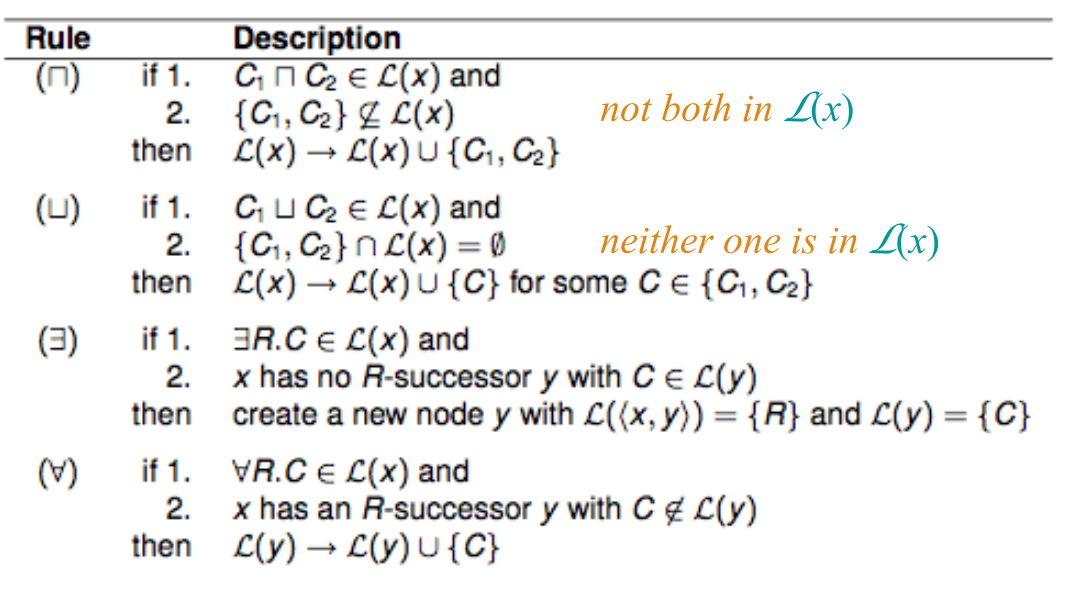
\includegraphics[width=\textwidth]{Images/rulesPropagation}
	\caption{Rules for constraint propagation}
	\label{img:rulesPropagation}
\end{figure}
In figure \ref{img:rulesPropagation} we have the rules for constraint propagation and also
most rules are deterministic, but the rule for disjunction is non deterministic: 
its application results in alternative constraints sets, so we have a fork in the proof.

$A$ is satisfiable iff at least one of the resulting constraint set is satisfiable, and 
$A$ is unsatisfiable iff all the alternatives end up with a clash.

The result is invariant with respect to the order of application of the rules, and we have
the following result for correctness and completeness:
\begin{description}
   \item [Correctness: ] if the algorithm terminates with at least one primitive constraint
	   set and no clashes, then $A$ is satisfiable and from the constraints
           we can derive a model.
   \item [Completeness: ] if a knoweldge base $A$ is satisfiable, then the algorithm
                          terminates producing at least a finite model without clashes.
\end{description}
We have $KBS$ decidable for $ALC$ and also for $ALCN$.

\begin{figure}
	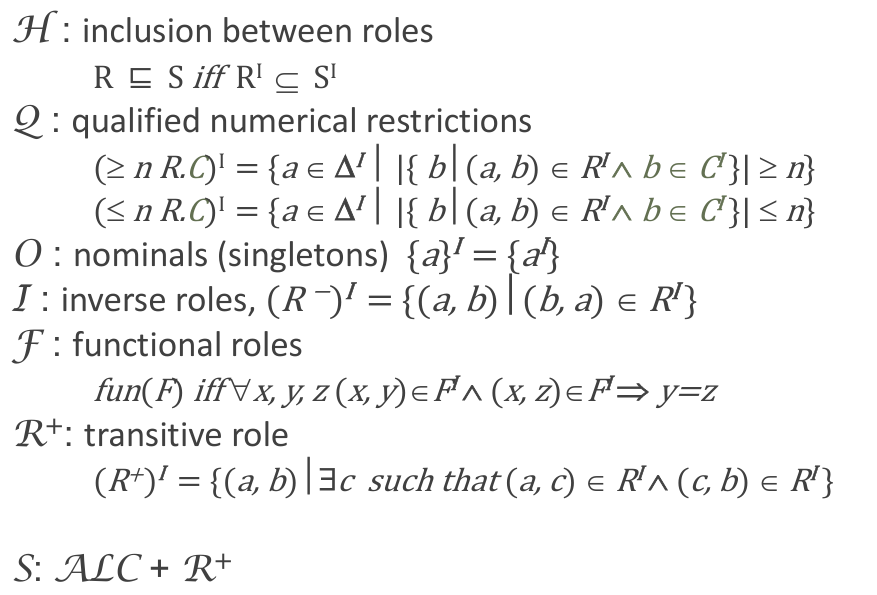
\includegraphics[width=\textwidth]{Images/addConstructors}
	\caption{Additional constructors to description logics}
	\label{img:addConstructors}
\end{figure}
In figure \ref{img:addConstructors} is possible to note possible additional constructors to
description logics, ans we have that \emph{OWL-DL} is equivalent to $SHOIN$, instead
\emph{OWL-Lite} is equivalent to $SHIF$; these two language are the ontology language
for Semantic Web.

\begin{figure}
	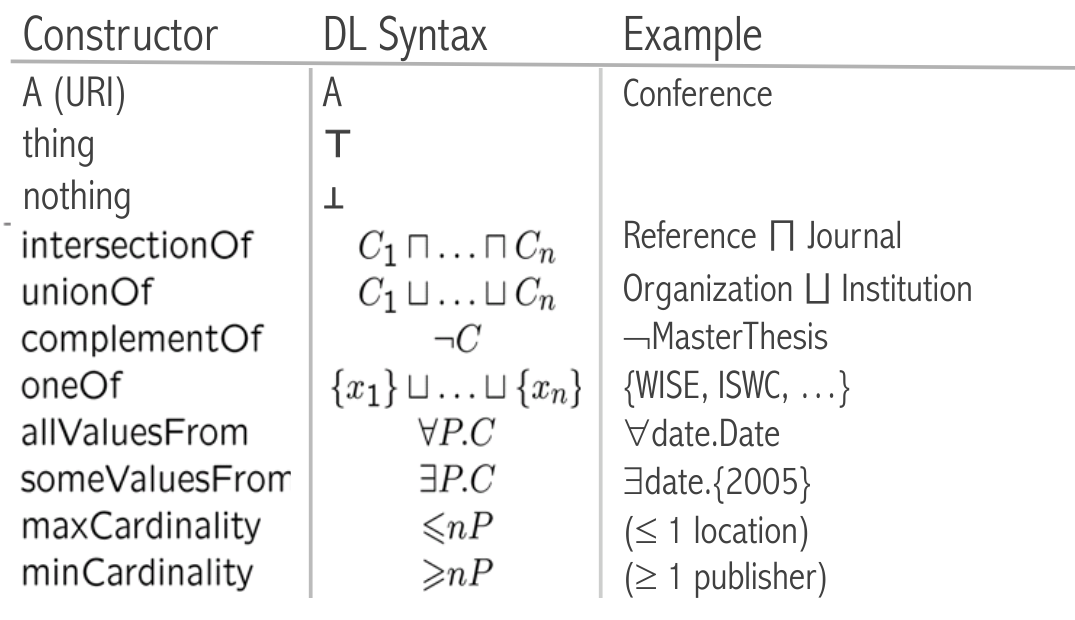
\includegraphics[width=\textwidth]{Images/owlSyntax}
	\caption{Syntax for OWL}
	\label{img:owlSyntax}
\end{figure}

\begin{figure}
	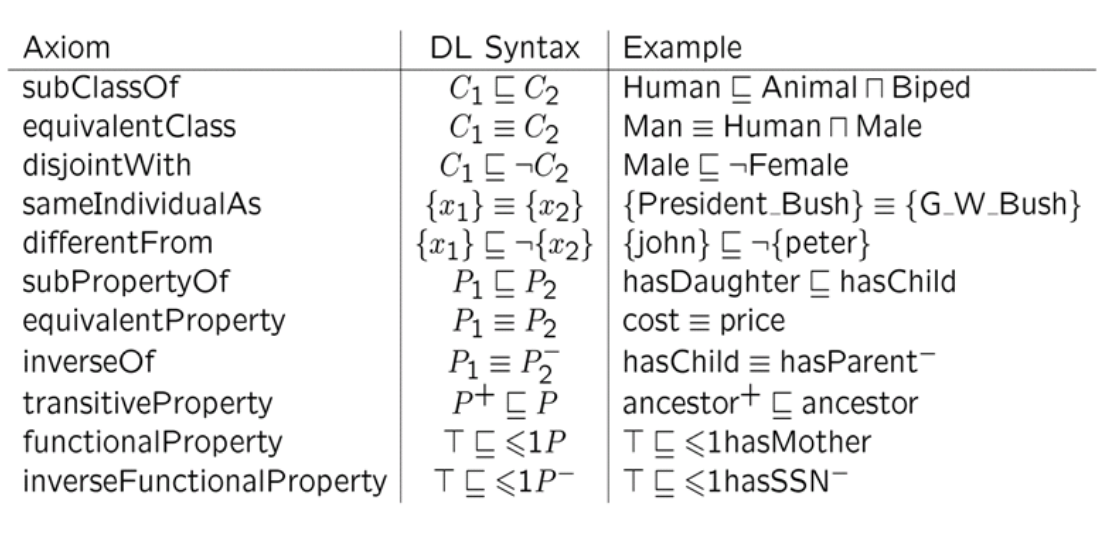
\includegraphics[width=\textwidth]{Images/owlAxioms}
	\caption{Axioms defined for OWL}
	\label{img:owlAxioms}
\end{figure}
The syntax for OWL is defined by figure \ref{img:owlSyntax}, axioms by figure 
\ref{img:owlAxioms}, the XML syntax used in visible in figure \ref{img:owlXML} and in the
end in figure \ref{img:DLresults} is possible to see complexity and decitability results
for DL's.

\begin{figure}
	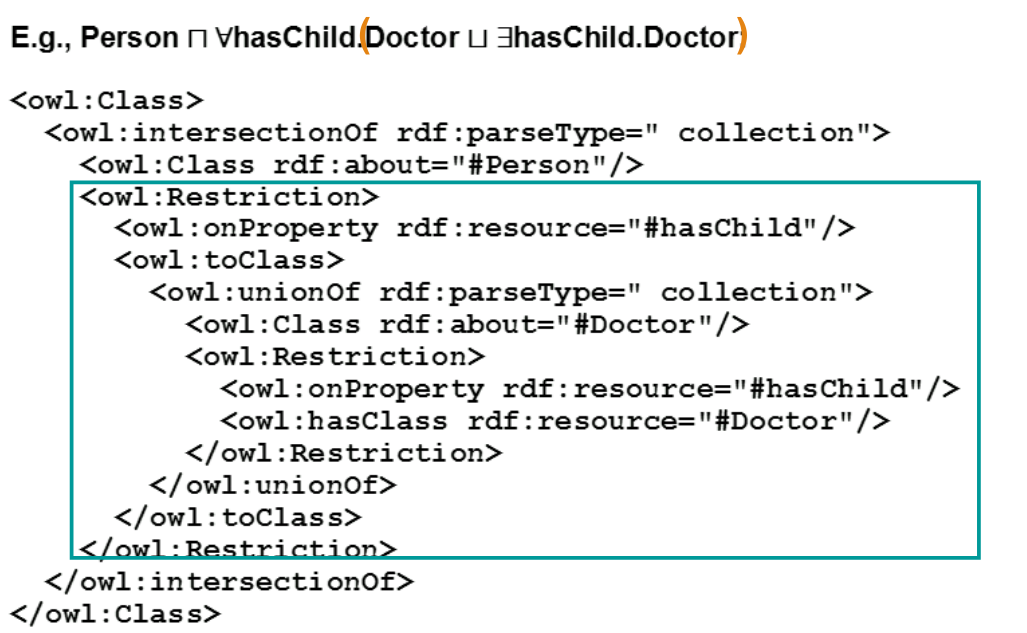
\includegraphics[width=\textwidth]{Images/owlXML}
	\caption{XML syntax used for OWL}
	\label{img:owlXML}
\end{figure}
\begin{figure}
	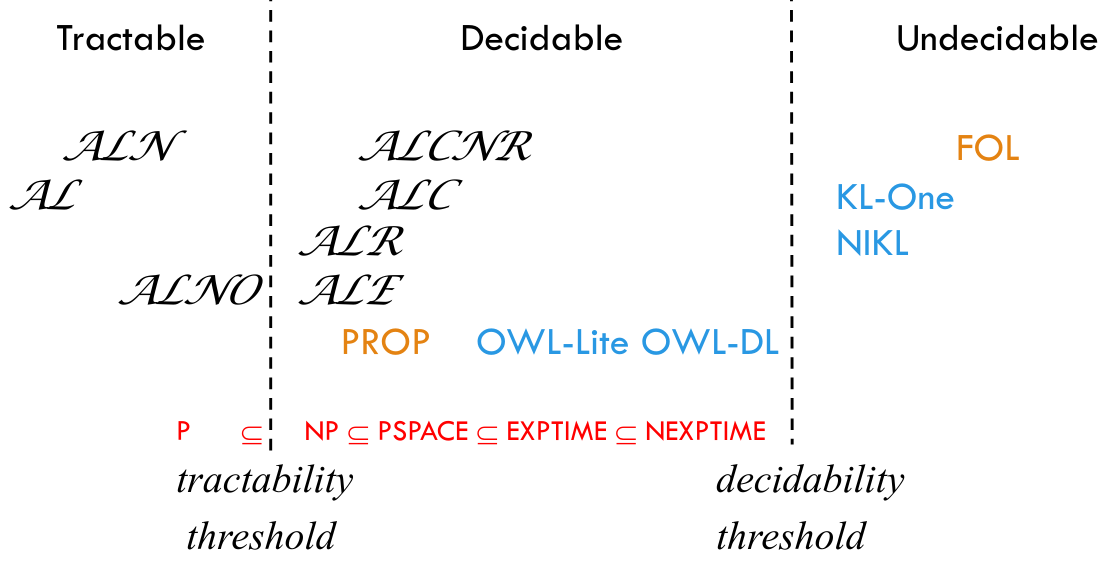
\includegraphics[width=\textwidth]{Images/DLresults}
	\caption{Complexity and decidability results for DL}
	\label{img:DLresults}
\end{figure}

%Knowledge Chapter
  \chapter{Bayesian Network}
In this chapter we will talk about Bayesian Network, but before we introduce and analyze
it we will refresh our knowledge of probability.

\section{Uncertain Reasoning}
Agents are inevitably forced to reason and make decisions based on incomplete information 
and they need a way to handle uncertainty deriving from:
\begin{enumerate}
   \item partial observability (uncertainty in sensors).
   \item nondeterministic actions (uncertainty in actions).
\end{enumerate}
A partial answer would be to consider, instead of a single world, a set of possible
worlds (those that the agent considers possible, so a belief set) but planning by
anticipating all the possible contingencies can be really complex.\newline
Moreover, if no plan guarantees the achievement of the goal, but still the agents
needs to act, we have that probability theory offers a clean way
to quantify uncertainty (common sense reduced to calculus).

Suppose the goal for a taxi-driver agent is "delivering a passenger to the airport
on time for the flight" and consider action $A_t = $ leave for airport $t$ minutes
before flight.\newline
How can we be sure that $A_{90}$ will succeed, because there are many sources of uncertainty:
\begin{enumerate}
   \item partial observability or noisy sensors: road state, other drivers plans,
	 police control, inaccurate traffic reports and so on.
   \item uncertainty in action outcomes (flat tire, car problems, bad weather and so on).
\end{enumerate}
With a logic approach it is difficult to anticipate everything that can go wrong
(qualification problem), $A_{90}$ may be the most rational action, given that the
airport is $5$ miles away and you want to avoid long waits at the airport and still
catch the flight.

The rational decision depends on both the relative importance of various goals
and the likelihood that, and degree to which, they will be achieved.\newline
When there are conflicting goals the agent may express preferences among
them by means of a utility function and utilities are combined with probabilities
in the general theory of rational decisions called \emph{decision theory}.\newline
An agent is rational if and only if it chooses the action that yields the maximum
expected utility, averaged over all the possible outcomes of the action.\newline
This is called the principle of \emph{Maximum Expected Utility} (MEU).

Logic theory and probability theory both talk about a world make of propositions which
are true or false and they share the ontological commitment.
What is different is the \emph{epistemological} commitment: a logical agent believes each
sentence to be true or false or has no opinion, whereas a probabilistic agent 
may have a numerical degree of belief between $0$ (for sentences that are certainly false)
and $1$ (certainly true).\newline
One example can be to define the patient who has a toothache 
has a cavity with $0.8$ probability.\newline
The uncertainty is not in the world, but in the beliefs of the agent (state of knowledge),
so if the knowledge about the world changes (we learn more information about the
patient) the probability changes, but there is no contradiction.

We assume now a knowledge of Probability, like conditional probabilities, Bayes formula, 
definition of probability and so on.\newline
We now refresh now how to compute the probability of a variable from the full joint
distribution, so given a joint distribution $P(X, Y)$ over variables $X$ and $Y$,
the distribution of the single variable $X$ is given by
\[ P(X) = \sum _{y \in dom(Y)} P(X, y) = \sum _y P(X, y) \]
This operation is also called \emph{marginalization}.
A variant of the marginalization rule, called \emph{conditioning}, involves conditional 
probabilities instead of joint probabilities.\newline
It can be obtained from marginalization using the product rule and it is 
\[ P(Y) = \sum _{z \in Z} P(Y | z) P(z) \]
If the query involves a single variable $X$, $e$ is the list of the observed values and 
$Y$ the rest of unobserved variables, we have that 
\[ P(X | e) = \alpha P(X, e) = \alpha \sum_y P(X, e, y) \]
However the complexity of the joint distribution table is intractable, so if $n$ is the 
number of boolean variables, it requires an input table of size $O(2^n)$ and requires
$O(2^n)$ time to process.\newline
Better reasoning involves using Bayes theorem or leveraging on the notion of independence,
that can reduce the size of representation.\newline
Bayes rule tells us how to update the agent's belief in hypothesis $h$ as new evidence
$e$ arrives, given the background knowledge $k$, as follows
\[ P(h | e, k) = \frac{P(e | h, k) P(h | k)}{P(e | k)} \]
We define a refinement of the independence property, called \emph{conditional independece},
which is defined that $X$ and $Y$ are conditionally independent given $Z$, when 
\[ P(X, Y | Z) = P(X | Z) P(Y | Z) \]
Using product rule and conditional independence is possible to obtain this alternative 
formulation which estabilish that $X$ and $Y$ are conditionally independent given $Z$ when
\[ P(X | Y, Z) = P(X | Z) \]
\[ P(Y | X, Z) = P(Y | Z) \]
We also cite \emph{Naive Bayes model}, used in Naive Bayes classifiers, where the full joint
distribution can be computed as 
\[ P(Cause, Effect_1, Effect_2, \dots, Effect_n) = P(Cause) \prod _i P(Effect_i | Cause) \]
This distribution can be also be obtained from observations, anyway better explanation
will be provided in other courses, like Intelligent Systems for Pattern Recognition.

\section{Bayesian Network}
\emph{Bayesian networks} (also called belief networks) are graphs for representing
dependencies among variables and the network makes explicit conditional dependencies:
the intuitive meaning of an arc from $X$ to $Y$ is typically that
$X$ has a direct influence on $Y$.\newline
Bayesian networks are directed acyclic graphs (DAG) so defined:
\begin{enumerate}
   \item Each node corresponds to a random variable, which may be discrete or continuous.
   \item Directed links or arcs connect pairs of nodes and if there is an arc from node $X$
	 to node $Y$ , $X$ is said to be a parent of $Y$.\newline
	 Parents ($Y$) is the set of variables directly influencing Y.
   \item Each node $X$ has an associated conditional probability distribution table
	 $P(X | Parents(X))$ that quantifies the effect of the parents on the node.
\end{enumerate}
Easier for domain experts to decide what direct influences exist in the domain than
actually specifying the probabilities themselves and the network naturally represents
independence and conditional independence, infact the lack of an arc connection between 
two variables is interpreted as \emph{independence}.

We define now two alternative and equivalent ways to look at
the semantics of Bayesian networks:
\begin{enumerate}
   \item Distributed representation of the full joint probability distribution, which
	 suggests a methodology for constructing networks.
   \item An encoding of a collection of conditional independence statements, which
	 helps in designing inference procedures.
\end{enumerate}
A Bayesian network can be seen as a representation of the full joint distribution, since
a joint probability distribution can be expressed in terms of conditional probabilities
\[ P(x_1, \dots, x_n) = P(x_n | x_{n-1}, \dots, x_1) P(x_{n-1}, \dots, x_1) \]
By iterating the process we get the so-called chain rule
\begin{align*}
	P(x_1, \dots, x_n) & = P(x_n | x_{n-1}, \dots, x_1) P(x_{n-1} | x_{n-2} \dots x_1)
	                      \dots P(x_2 | x_1) P(x_1) \\
			   & = \prod _{i=1}^n P(x_i | x_{i-1}, dots, x_1)
\end{align*}
This amounts to assuming an ordering of the variables, computing the posterior probabilities
of each variable, given all previous variables and in the end 
taking the product of these posteriors.

Assuming that each variable appears after its parents in the ordering, we simplify
the computation by conditioning the computation only to values of the parent variables
(assuming the others are independent) and the numbers in the CPT's
are actually conditional probabilities.\newline
Each entry in the joint distribution can be computed as the product of the
appropriate entries in the conditional probability tables (CPTs) in the Bayesian network.

We get the simplified rule for computing joint distributions 
\[ P(x_1, \dots, x_n) = \prod _{i=1}^n P(x_i | parents(X_i)) \]
where $parents(X_i)$ denotes the set of values $x_1, \dots, x_n$ for $parents(X_i)$.\newline
A Bayesian network is a distributed representation of the full joint distribution.

We present now a procedure for building a Bayesian network which is a good representation
of a domain:
\begin{description}
   \item [Nodes: ] determine the set of variables required to model the domain and we 
	   order them in $\{X_1, \dots, X_n\}$.\newline
	   Ordering influences the result: the resulting network will be more compact
	  if the variables are ordered such that causes precede effects.
   \item [Links: ] For $i = 1$ to $n$ choose from $X_1, \dots, X_{i-1}$ a minimal set of
	   parents for $X_i$, such that equation 
	   \[ P(X_i | X_{i-1}, \dots, X_1) = P(X_i | Parents(X_i) \]
	   is satisfied.\newline
	   For each parent insert an arc from the parent to $X_i$ and write down the 
	   conditional propability table $P(X_i | Parents(X_i))$.
\end{description}
Note that the parents of node $X_i$ should contain all those nodes in 
$X_1, \dots, X_{i-1}$ that directly influence $X_i$ and also note that the network 
is a DAG by construction and contains no redundant probability values.

If we use a causal model (with links from causes to effect) we obtain a better network,
with less connections (more compact), fewer probabilities to specify and
the numbers will often be easier to obtain.\newline
In locally structured systems, each subcomponent interacts directly with only a
bounded number of other components and this is a huge savings
wrt full joint distribution tables.

Locally structured domains are usually associated with linear rather than exponential
growth in complexity, and in the case of Bayesian networks, it is reasonable 
to suppose that in most domains each random variable is directly influenced by 
at most $k$ others, for some constant $k$.\newline
If we assume $n$ Boolean variables, then each conditional probability table will have at
most $2^k$ numbers, and the complete network can be specified by $n2^k$ numbers, in
contrast, the joint distribution contains $2^n$ numbers.

We can also extract the independence assumptions encoded in the graph structure 
to do inference and the topological semantics specifies that each variable
is conditionally independent of its non-descendants, given its parents.\newline
A node X is conditionally independent of all other nodes in the network given its parents,
children, and children’s parents and this is its Markov blanket.

Often the relationship between a node and its parent follows a canonical
distribution and the construction of the CPT’s can be simplified, so we present
two examples:
\begin{description}
   \item [Deterministic nodes: ] nodes whose value is specified exactly by the 
	   values of their parents.
   \item [Noisy-OR relations: ] a generalization of the logical OR, so for example we can 
	   define the following proposition
	   	\[ Cold \lor Flu \lor Malaria \iff Fever \]
		We can specify inhibiting factors for Cold, Flu, Malaria and we have two
		assumpions with Noisy-OR:
		\begin{itemize}
			\item all the possible causes are listed; if not, we can add a 
			      leak condition/node.
			\item the inhibiting factor of each parent is independent of any
			      other parent.
		\end{itemize}
\end{description}
One possible way to handle continuous variables (such as temperature) is to avoid
them by using discrete intervals, but the most common solution is to define standard
families of probability density functions that are specified 
by a finite number of parameters, like for example a normal distribution $N(\mu, \sigma^2)$.

A network with both discrete and continuous variables is called a
\emph{hybrid Bayesian network}.\newline
Hybrid Bayesian networks combine discrete and continuous variables and there are 
two new kinds of distributions:
\begin{enumerate}
   \item the conditional distribution for a continuous variable given discrete
         and continuous parents.
   \item the conditional distribution for a discrete variable given continuous parents.
\end{enumerate}
Given $X$, the query variable (we assume one), $E$ the set of evidence variables $\{E_1, 
\dots, E_m\}$, and $Y$ the set of unknown variables, a typical query asks for $P(X | E)$.

We defined a procedure for the task by enumeration as 
\[ P(X | e) = \alpha P(X, e) = \alpha \sum_t P(X, e, y) \]
where $\alpha$ is a normalization factor.\newline
The query can be answered using a Bayesian network by computing sums of products of
conditional probabilities from the network.

\begin{figure}
	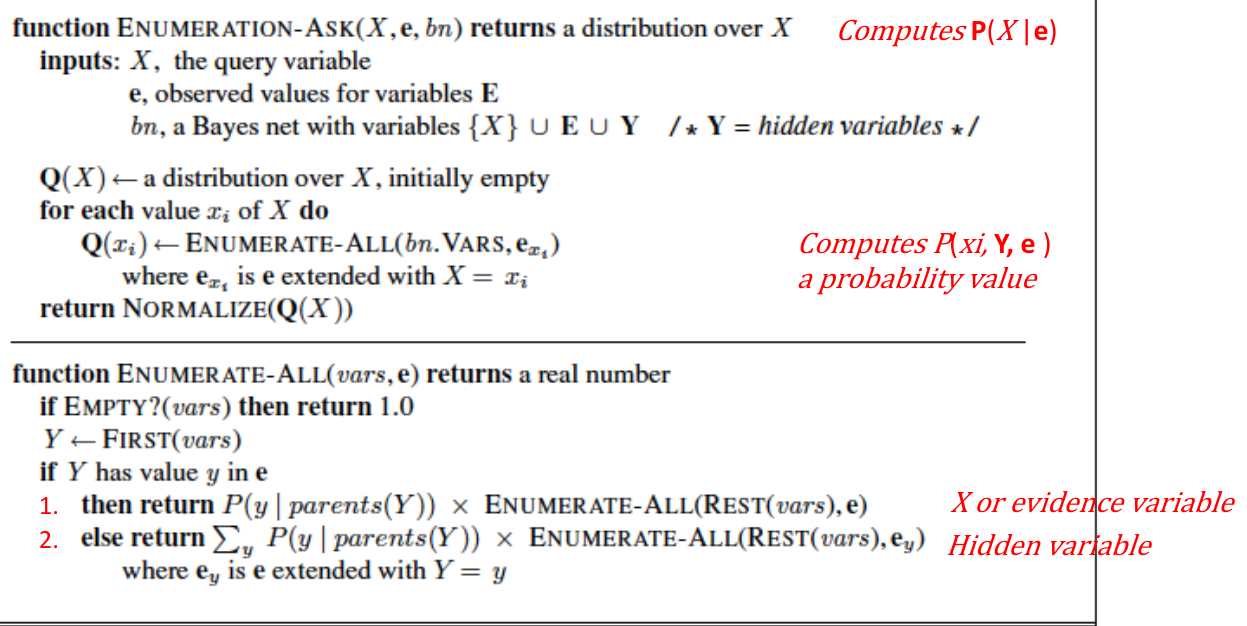
\includegraphics[width=\textwidth]{Images/enumerationAsk}
	\caption{Pseudocode for Enumeration Ask}
	\label{img:enumerationAsk}
\end{figure}
In figure \ref{img:enumerationAsk} there is the pseudocode for the inference procedure 
using enumeration, that can be improved substantially, by storing and reusing the
results of repeated computations (a kind of dynamic programming).\newline
The variable elimination algorithm, proceeds right-to-left (bottom-up) and 
conditional probabilities are represented as factors, matrices resulting from conditional
probabilities and the names make explicit the argument.\newline
For example if we have $P(a | b, e)$ we define the factor $f_i(a, b, e)$ and 
two operations on factors: pointwise-product $(x)$ and summing out variables.

Given a variable and some evidence, a factor can be built by looking at the variable part
of CPTS’s in the network, using $\proc{MAKE-FACTOR(var, e)}$ and the 
\emph{pointwise product} of two factors $f_1$ and $f_2$ yields a new factor $f_3$
such that variables are the union of the variables in $f_1$ and $f_2$ and
elements are given by the product of the corresponding values in the two factors, so
for example computation of the poitnwise product $f_1(A, B) \times f_2(B, C)$ gives
$f_3(A, B, C)$ and the result is not necessarily a probability distribution.

Computational saving comes from the realization that any factor that does not depend
on the variable to be summed out can be moved outside the summation and this operation
of "distributing out" common factors is part of the operation, which in
the general case returns a set of factors.\newline
In figure \ref{img:improvedEliminationAsk} is possible note this improved version of 
variable elimination, where $\proc{MAKE-FACTOR}$ creates a factor for each variable,
given the evidence and $\proc{SUM-OUT}$ sums out over the possible values of a hidden variable,
producing a set of factors; it takes care of distributing out factors 
which do not depend on the variable.

\begin{figure}
	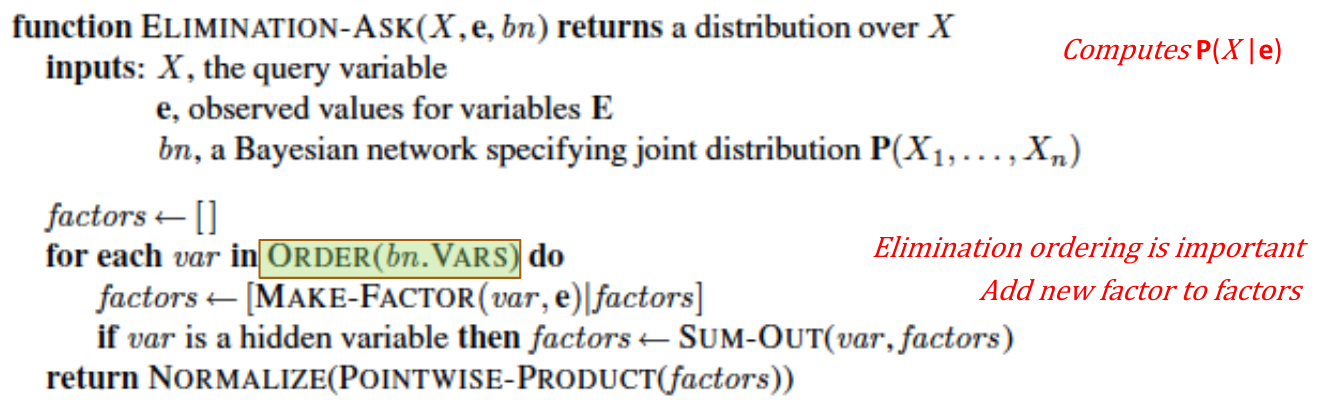
\includegraphics[width=\textwidth]{Images/variableElimination}
	\caption{Pseudocode for Variable elimination algorithm}
	\label{img:improvedEliminationAsk}
\end{figure}
Every choice of ordering yields a valid algorithm, but different orderings of variables
can produce differences in efficiency, but determining the optimal ordering is intractable,
but several good heuristics are available, for example eliminate whichever
variable minimizes the size of the next factor to be constructed.

We can remove any leaf node that is not a query variable or an evidence variable, and 
continuing this process, we can remove any variable that is not an ancestor of a query
variable or evidence variable.

The complexity of exact inference in Bayesian networks depends strongly on the structure
of the network, singly connected networks or polytrees are such that there
is at most one undirected path between any two nodes.\newline
The time and space complexity of exact inference in polytrees is linear in the size
of the network (the number of CPT entries).\newline
For multiply connected networks variable elimination can have exponential time and 
space complexity in the worst case, infact inference in Bayesian networks 
includes as a special case propositional inference, which is NP-complete.

\section{Probabilistic reasoning over time}
So far, we have been doing uncertain reasoning in a static world and for reasoning in an
evolving world an agent needs:
\begin{description}
   \item [belief state: ] the states of the world that are possible.
   \item [transition model: ] to predict how the world will evolve.
   \item [sensor model: ] to update the belief state from perceptions.
\end{description}
A changing world is modeled using a variable for each aspect of the world state at each point
in time (fluents) and we use probabilities to quantify how likely a world is.\newline
The transition and sensor model themselves may be uncertain:
\begin{itemize}
   \item the \emph{transition model} gives the probability distribution of the variables
	 at time $t$, given the state of the world at past times.
   \item the \emph{sensor model} describes the probability of each percept at time $t$,
	 given the current state of the world.
\end{itemize}
We view the world as a series of snapshots, or time slices, each of which contains a set of
random variables, some observable and some not.\newline
$X_t$ will denote the set of state variables, unobservable (hidden) at time $t$ and 
$E_t = e_t$ will denote the set of observations (evidence variables) at time $t$, with 
$e_t$ their values.\newline
We will assume that the state sequence starts at $t=0$ and the distance between time slices 
is fixed and we will use the notation $a:b$ to denote the sequence of integers 
from $a$ to $b$ (inclusive), and the notation $X_{a:b}$ to denote the set of variables
from $X_a$ to $X_b$.

The transition model specifies how the world evolves, the probability distribution over the
latest state variables, given the previous values starting from time $0$
\[ P(X_t | X_{0:t-1}) \]
The sequence of states can become very large, unbounded as $t$ increases and we define the 
\emph{Markov assumptions}: the transition model specifies the probability distribution
over the latest state variables, given a finite fixed number of previous states
\[ P(X_t | X_{0:t-1}) = P(X_t | X_{t-1}) \quad \text{first order Markov chain} \]
\[ P(X_t | X_{0:t-1}) = P(X_t | X_{t-1}, X_{t-2}) \quad \text{second order Markov chain} \]
Additionally, we assume a stationary process, so the conditional probability distribution
is the same for all $t$, since sometimes change is governed by laws that do not themselves
change over time.

\begin{figure}
	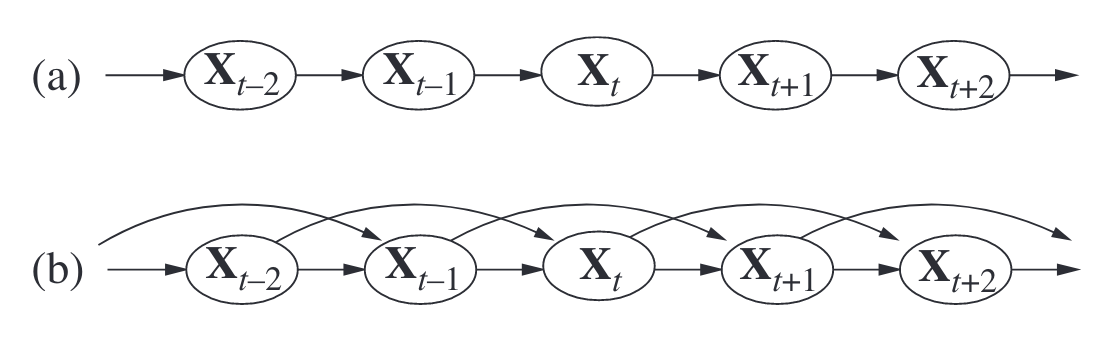
\includegraphics[width=\textwidth]{Images/bayesianMarkov}
	\caption{Bayesian Network of Markov chain}
	\label{img:bayesianMarkov}
\end{figure}
In figure \ref{img:bayesianMarkov} is possible note the transition model using Markov 
chain in Bayes networks and the sensor/observation model, under Markov sensor assumption,
postulates that evidence only depends on the current state
\[ P(E_t | X_{0:t}, E_{0:t-1}) = P(E_t | X_t) \]
This is a reasonable assumption to make, given the availability of sensors.\newline
Assuming for example that "Rain" only depends on rain the previous day may be a too strong
assumption, so there are two ways to improve the accuracy of the approximation:
\begin{enumerate}
    \item Increasing the order of the Markov process model, for example using
	  a second order assumption.
    \item Increasing the set of state variables: we could add Season, Temperature, Humidity,
          Pressure and so on as state variables.\newline
	  This may imply more computation for predicting state variables or adding new sensors.
\end{enumerate}
We also need the prior probability distribution at time $0, P(X_0)$, so putting all together,
the complete joint distribution over all the variables, for any $t$, 
computed from the network is
\[ P(X_{0:t}, E_{1:t}) = P(X_0) \prod _{i=1}^t P(X_i | X_{i-1}) P(E_i | X_i) \]

Basic inference tasks based on the temporal model, consist in the following operations:
\begin{description}
   \item [Filtering:]  computing the belief state (posterior probability distribution of 
	   state variables) given evidence from previous and current states.\newline
	   A subtask is the likelihood of the evidence sequence $P(X_t | e_{1:t})$.
   \item [Prediction: ] computing the posterior distribution over a future state, given all
          evidence to date, so we compute $P(X_{t+k} | e_{1:t})$ with $k > 1$.
   \item [Smoothing: ] computing the posterior distribution over a past state, given all
	   evidence up to the present.\newline
	   Looking back with the knowledge of today provides a more accurate estimate, so
	   we have $P(X_k |e_{1:t})$ with $0 \leq  k < t$.
   \item [Most likely explanation/sequence: ] given a sequence of observations, we might wish
       to find the sequence of states that is most likely to have generated those observations.
   \item [Learning: ] the transition and sensor models, can be learned from observations.
\end{description}
\begin{figure}
	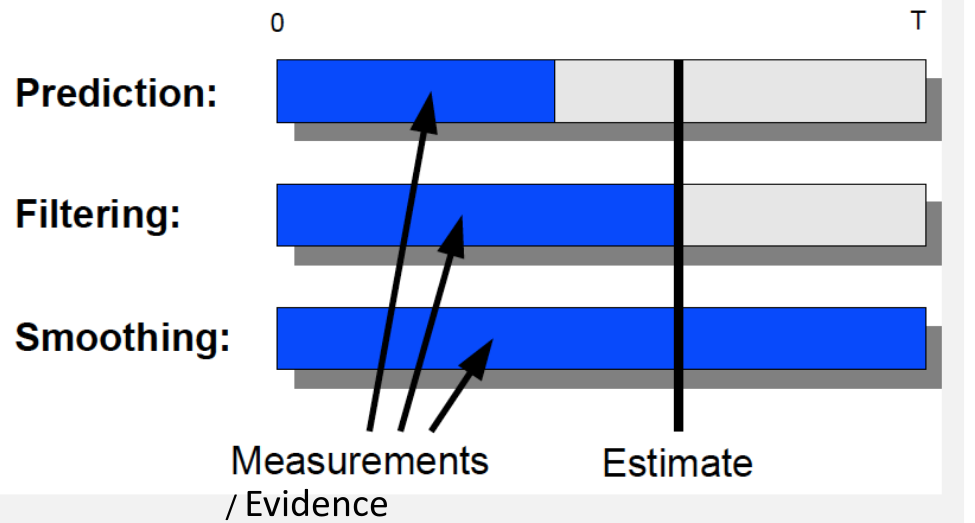
\includegraphics[width=\textwidth]{Images/inferenceOperations}
	\caption{Interaction between time and inference operations}
	\label{img:filtering}
\end{figure}
In figure \ref{img:filtering} is possible to note how some inference operations interface
with past, current and future state and a good filtering algorithm maintains a current state
estimate and updates it, rather than going back over the entire history of percepts
for each time.\newline
The filtering function $f$ takes into account the state estimation computed up to the
present and the new evidence.
\[ P(X_{t+1} | e_{1:t+1}) = f(e_{t+1}, P(X_t | e_{1:t}) \]
This process is called \emph{recursive estimation} and is made of two parts:
\begin{description}
   \item [Prediction: ] the current state distribution is projected forward from $t$ to $t+1$:
	   \[ P(X_{t+1} | e_{1:t}) \]
   \item [Update: ] it is updated using the new evidence $e_{t+1} P(e_{t+1} | X_{t+1})$.
\end{description}
Filtering can be computed as follows:
\begin{align*}
    P(X_{t+1} | e_{1:t+1}) & = P(X_{t+1} | e_{1:t}, e_{t+1}) \\
	                   & = \alpha P(e_{t+1} | X_{t+1}, e_{1:t}) P(X_{t+1} | e_{1:t}) \\
			   & = \alpha P(e_{t+1} | X_{t+1}) P(X_{t+1} | e_{1:t}) \\
			   & = \alpha P(e_{t+1} | X_{t+1}) \sum_{x_t} P(X_{t+1}| x_t, e_{1:t})
			                                               P(x_t | e_{1:t}) \\
			   & = \alpha P(e_{t+1}|X_{t+1}) \sum_{x_t} P(X_{t+1} | x_t) 
			                                            P(x_t | e_{1:t}) \\
\end{align*}
We can think of $P(X_t|e_{1:t})$ as a message $f_{1:t}$ that is propagated forward
in the sequence and this makes evident the recursive structure:
\[ f_0 = P(X_0) \]
\[ f_{1:t+1} = \alpha Forward(f_{1:t}, e_{t+1}) \]
where $Forward$ implements the filtering update in constant time.

The task of prediction can be seen simply as filtering without the contribution of new
evidence and also the filtering process already incorporates a one-step prediction.\newline
In general, looking ahead $k$ steps, at time $t+k+1$, given evidence up to $t$ is done by
\[ P(X_{t+k+1} | e_{1:t}) = \sum _{x_{t+k}} P(X_{t+k+1} | x_{t+k}) P(x_{t+k} | e_{1:t}) \]
This computation involves only the transition model and not the sensor model and 
we can show that the predicted distribution for Rain converges to a fixed point $(0.5, 0.5)$,
after which it remains constant for all time (the stationary distribution of the
Markov process).\newline
The \emph{mixing time} is the time to reach the fixed point and we have that the more
uncertainty there is in the transition model, the shorter will be the mixing time
and the more the future is obscure.

We can use a forward recursion also to compute the likelihood of an evidence sequence
P e 1:t , useful if we want to compare two models producing the same evidence sequence.\newline
We can derive a recursive equation similar to filtering and a similar likelihood message
\[ l_{1:t}(X_t) = P(X_t, e_{1:t}) \]
Once we have $l_{1:t}(X_t)$ we can compute the likelihood of the evidence sequence by
summing out on the values of $X_t$ as follows
\[ L_{1:t} = P(e_{1:t}) = \sum _{x_t} l_{1:t}(x_t) \]
Note that the likelihood becomes smaller and smaller as $t$ increases.

Smoothing is the process of computing the posterior distribution of the state at some
past time $k$ given a complete sequence of observations up to the present $t$
\[ P(X_k | e_{1:t}) \quad \text{for } 0 \leq k < t \]
The additional evidence is expected to provide more information and more accurate
predictions on the past.

To compute the smoothing we have the following phases
\begin{align*}
   P(X_k | e_{1:t}) & = P(X_k | e_{1:k}, e_{k+1:t}) \\
	            & = \alpha P(X_k | e_{1:k}) P(e_{k+1:t} | X_k, e_{1:k}) \\
		    & = \alpha P(X_k | e_{1:k}) P(e_{k+1:t} | X_k) \\
		    & = \alpha f_{1:k} \times b_{k+1:t} \\
\end{align*}
$P(X_k|e_{1:k})$ corresponds to the forward message $f_{1:k}$, computed up to $t$,
as before in filtering and we define another message $b_{k+1:t} = P(e_{k+1:t}|X_k)$ 
that can be computed by a recursive process that runs backward from $t$.\newline
The terms in $f_{1:k}$ and $b_{k+1:t}$ can be implemented by two recursive calls,
one running forward from $1$ to $k$ and using the filtering equation and 
the other running backward from $t$ to $k+1$ for computing $P(e_{k+1:t}|X_k)$.

To compute smoothing going backwards we have 
\begin{align*}
   P(e_{k+1:t} | X_k) & = \sum _{x_{k+1}} P(e_{k+1:t}|X_k, x_k+1) P(x_{k+1}|X_k) \\
	              & = \sum _{x_{k+1}} P(e_{k+1:t}|x_{k+1}) P(x_{k+1}|X_k) \\
		      & = \sum _{x_{k+1}} P(e_{k+1}, e_{k+2:t} | x_{k+1}) P(x_{k+1} | X_k) \\
		      & = \sum _{x_{k+1}} P(e_{k+1} | x_{k+1}) P(e_{k+2:t} | x_{k+1})
		                          P(x_{k+1} | X_k) \\
\end{align*}
$b_{k+1:t} = P(e_{k+2:t}|x_{k+1})$ is defined by the previous equation computing backward
and the backward phases start with $b_{t+1:t} = 1$ and then we compute 
\[ b_{k+1:t} = Backward(b_{k+2:t}, e_{k+1}) \]
where $Backward$ implements the update defined above.

To improve efficincy we use an algorithm, called \emph{forward–backward}, visible in figure
\ref{img:forwardBackward}, which uses dynamic programming to reduce the complexity
of running the algorithm over the whole sequence.\newline
The trick is to record the results computed during the forward filtering phase,
over the whole sequence, and reuse them during the backward phase, so we obtain that 
the complexity is $O(t)$ and is consistent with the fact that the 
Bayesian network structure is a polytree.\newline
The forward–backward algorithm is the basis for many applications that deal
with sequences of noisy observations and improvements are required to deal with
space complexity for long sequences and online computations, where new observations
continuously arrive (fixed-lag smoothing).

\begin{figure}
	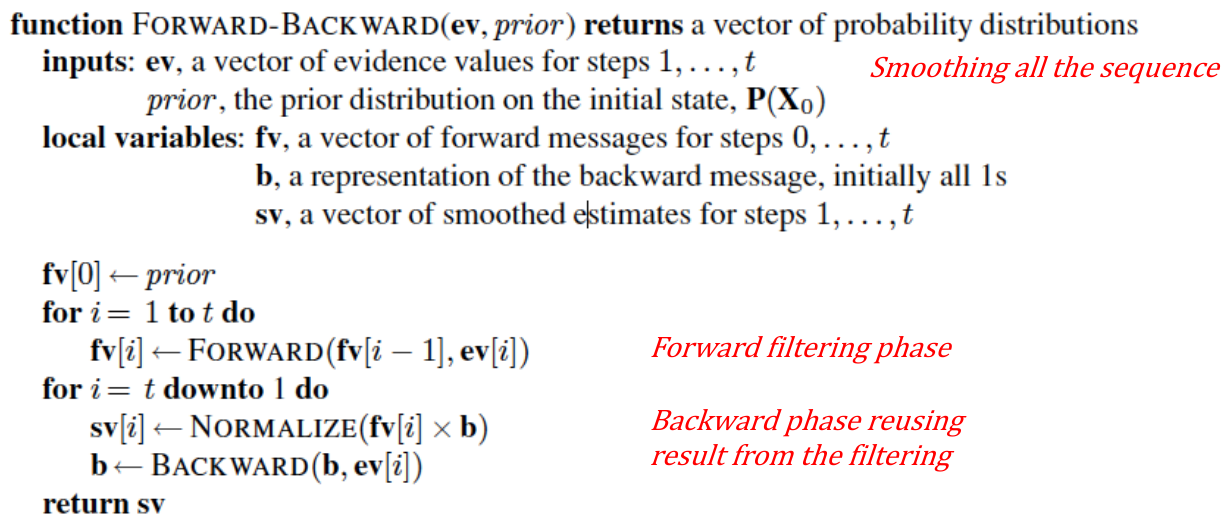
\includegraphics[width=\textwidth]{Images/forwardBackward}
	\caption{Pseudocode for ForwardBackward algorithm}
	\label{img:forwardBackward}
\end{figure}
Suppose we observe [ true, true, false, true, true ] for the Umbrella variable, so 
what is the most likely sequence for Rain given these oservations?\newline
There are $2^5$ possible Rain sequences, and each sequence is a path through a graph
whose nodes are the possible states at each time step.\newline
We want to discover which is the one maximizing the likelihood, in linear time and the 
likelihood of a path is the product of the transition probabilities along the path and
the probabilities of the given observations at each state.

There is a recursive relationship between the most likely path to each state $x_{t+1}$ 
and most likely paths to each previous state $x_t$.\newline
We can write a recursive equation, similar to the one for filtering as 
\[ \max_{x_1, \dots, x_t} P(x_1, \dots, x_t, X_{t+1} | e_{1:t+1}) = 
   \alpha P(e_{t+1} | X_{t+1}) \max_{x_t} (P(X_{t+1}|X_t) \max_{x_1, \dots, x_{t-1}}
   P(x_1, \dots, x_{t-1}, x_t | e_{1:t})) \]
The forward message in this case is $\max P(x_1, \dots, x_{t-1}, X_t | e_{1:t})$,
the probabilities of the best path to each state $x_t$; from those we can compute
the probabilities of the extended paths at time $t+1$ and take the max.\newline
The most likely sequence overall can be computed in one pass and for each state,
the best state that leads to it is recorded (marked as black arrows in the example)
so that the optimal sequence is identified by following black arrows backwards from the best
final state.\newline
This algorithm is the famous \emph{Viterbi algorithm}, named after A. Viterbi [1967]

The original application of Viterbi was in telecommunications: Viterbi decoders are used
for decoding a bitstream encoded using a technique called convolutional code or trellis code,
but is also used in NLP as different kinds of "sequence tagger" or also Speech recognition
(speech-to-text), speech synthesis, speech diarization.

We now present an overview of other approaches:
Probability theory and Bayesian networks are the dominant approaches today, despite
the disadvantage of having to specify many probability values (lots of numbers), so
other approaches are used to help humans to understand reasoning behind:
\begin{enumerate}
    \item Rule-based methods for uncertain reasoning in expert systems.
    \item Representing ignorance: Dempster–Shafer theory.
    \item Representing vagueness: fuzzy sets and fuzzy logic.
\end{enumerate}
Three good properties of classical logic-based rules:
\begin{description}
    \item [Locality: ] In logical systems, from $A$ and $A \to B$, we can conclude $B$,
	              without worrying about any other rules, instead in probabilistic systems,                      we need to consider all the evidence.
   \item [Detachment: ] once $B$ is proved, it can be used regardless of how it was derived and
	               it can be detached from its justification.
   \item [Truth-functionality: ] the truth of complex sentences can be computed from the
	          truth of the components, instead probability combination
		  does not work this way.
\end{description}
In Rule-based methods the idea is to attach degree of belief to facts and rules and 
to combine and propagate them, and the most famous example is the certainty factors model,
which was developed for the MYCIN medical diagnosis program.\newline
The system was carefully engineered to avoid mixing different kind of rules 
(diagnostic vs causal), trying to control non plausible results.

The theory of \emph{fuzzy sets} is a way to specify how well an object satisfies a vague
description (non categorical) property, like "being tall".\newline
Fuzziness is not uncertainty in the world, but is the uncertainty
in the use of qualifiers/properties.\newline
Fuzzy logic is way of reasoning about membership in fuzzy sets and a fuzzy predicate
implicitly defines a fuzzy set.\newline
Fuzzy logic is a method for reasoning with logical expressions describing
membership in fuzzy sets and standard rules used are 
\[ T(A \land B) = \min (T(A), T(B)) \]
\[ T(A \lor B) = \max (T(A), T(B)) \]
\[ T(\neg A) = 1 - T(A) \]

Fuzzy control is a methodology for constructing control systems in which the mapping
between real-valued input and output parameters is represented by fuzzy rules.\newline
It consist on the following operations:
\begin{description}
    \item [Fuzzification: ] continous variables are mapped into a set of linguistic variables
	    with fuzzy values; temperature can be mapped in fuzzy variables such as 
	    low, medium, high and their membership functions.
    \item [Reasoning: ] with rules expressed in terms of these fuzzy variables,
	    reaching fuzzy conclusions.
    \item [Defuzzification: ] map the results into numerical valueo far,
	   we have been doing uncertain reasoning in a static world.
\end{description}
%Bayesian Network Chapter
  \chapter{Rule-based systems}
We introduce now rule-based systems, which are a contractions of PROP and FOL, since 
by limiting expressivity to a specific interesting subset of first-order logic, resolution
procedures become much more manageable.\newline
We limit the degree of uncertainty we can express by considering clauses that have at
most one positive literal, \emph{Horn clauses}.\newline
We have two cases:
\begin{enumerate}
   \item The KB is a set of definite Horn clauses (exactly one positive literal),
	 written as $a_1 \land a_2 \land \dots \land a_m \Rightarrow h$, where rules
	 happens when $m > 0$ and facts are when $m = 0$.
   \item Goals or queries include only negative literals (negative clauses).
\end{enumerate}
We have limited expressivity, so we cannot represent disjunctive conclusions and also 
Propositional Horn clauses KB's have linear-time deduction algorithms.

Once we have a KB of fact and rules the inference procedure can work in two directions:
\begin{description}
   \item [Forward reasoning: ] use of rules from antecedent to consequent to compute
          all the logical consequences of the initial facts (also called bottom-up) and 
	  it is used in deductive databases, like Datalog, and in Production systems.
   \item [Backward reasoning: ] use of the rules from the consequent to the antecedent
          until goals match initial facts (also called top-down) and the most effective
	  strategy is called SLD and is used in Logic programming languages and PROLOG.
\end{description}
We start considering the forward reasoning, so for the first-order case inference 
is performed on the basis of the following rule, which makes use of unification:
\[ \frac{p_1', p_2', \dots, p_n' \, (p_1 \land p_2 \land \dots \land p_n \Rightarrow q)}
        {q \gamma} \]
where $\gamma$ is an MGU such that $p_i' \gamma = p_i \gamma$ for each $i$.
At each iteration new sentences are added to the KB and terminates when no 
new sentences are generated (fixed point) or goal is found.\newline
This inferential process is sound, the rule is correct and complete for Definite Horn clauses,
for Datalog databases (without function symbols, only constants) convergence is
also guaranteed since there are a finite number of consequences.

\begin{figure}
	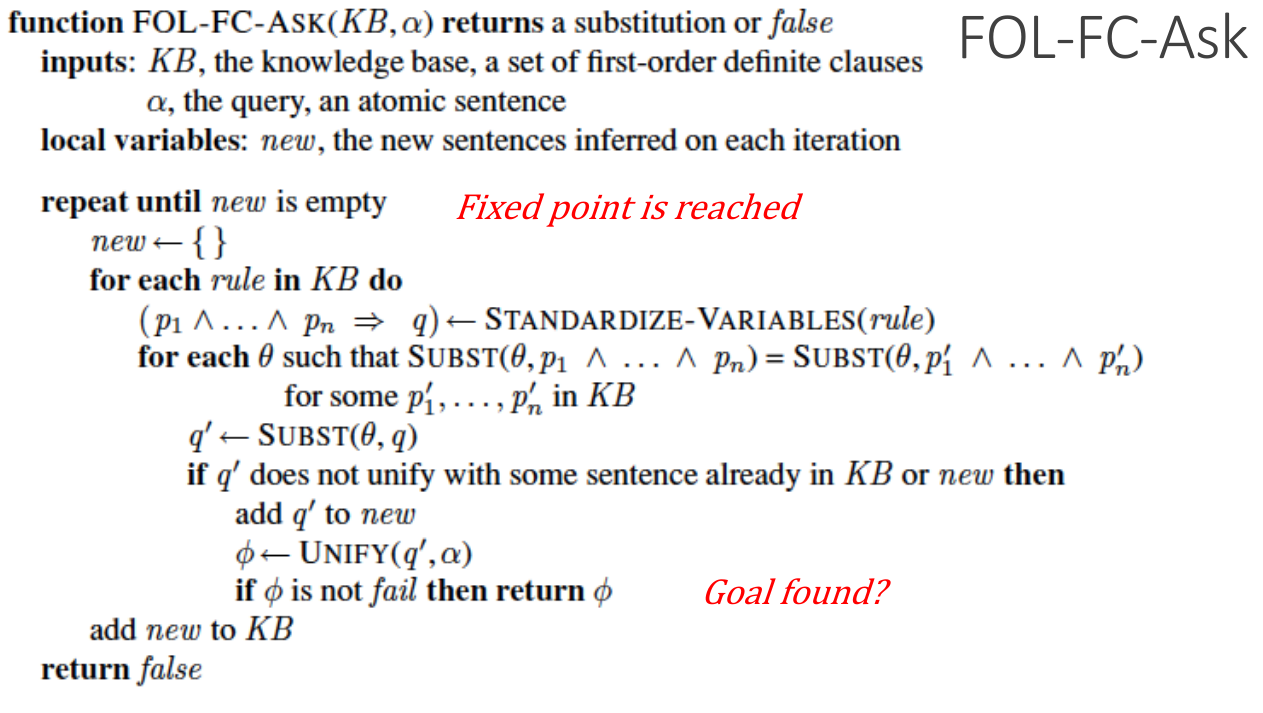
\includegraphics[width=\textwidth]{Images/forwardChaining}
	\caption{Pseudocode for Forward chaining}
	\label{img:forwardChaining}
\end{figure}
In figure \ref{img:forwardChaining} is possible to note the pseudocode for Forward chaining
and the interpreter is required to perform many unification operations, so if we have
$r$ rules to try (in OR), $n$ preconditions in each rules to be satisfied (in AND) and 
$w$ facts in the KB (in OR) and everything repeated for c cycles so we have 
$r \times n \times w \times c$ unification operations.

Finding all the facts that unify with a given pattern can be made more efficient 
with appropriate predicate indexing, so a hash table on the head of the predicate,
in the simplest case, but in complex case we can use a hash table with a combined key head
$+$ first argument and/or a discrimination network on the antecedents of the rules.\newline
Another improvents is that each rule does not need to be checked again at each iteration, so
only the ones which are affected by recent additions.
This two strategies are among the strategies implemented by the RETE algorithm included
in Production Systems and rule-based programming languages such as CLIPS.

Another improvement is the \emph{Conjunct ordering}, which the order in which you list
antecedents of rules is important for efficiency.\newline
Each antecedent is a constraint and each rule a CSP, so we can apply heuristics from CSP for
ordering and we can try to write rules which correspond to CSP with a tree-structure.\newline
The last improvement is that proceeding forward may lead to derive many irrelevant facts,
so we restrict the forward chaining to the relevant rules for the goal by proceeding backward
and marking them (in deductive databases are called \emph{Magic sets}).

Rule-based systems are one of the first paradigms for representing knowledge in A.I. and 
most expert systems are rule-based.\newline
Rules are used forward to produce new facts, hence the names productions and production systems
and they are a general computational model based guided by patterns: the rule to be applied
next is determined by the operation of pattern matching, a simplified form of unification.

CLIPS (C Language Integrated Production System”) is a successor of OPS-5 (Forgy), 
developed by NASA and now freely available at \href{http://www.clipsrules.net/}.

A typical rule-based system has four basic components:
\begin{enumerate}
   \item A list of facts (no variables), the temporary \emph{Working Memory} (WM), defined as 
	   \begin{lstlisting}
	   (predicate arg_1 arg_2 \dots arg_k) %ordered facts 
	   (predicate (slot_1 val_1) \dots (slot_k val_k)) %structured facts}
	   \end{lstlisting}
   \item A list of rules or rule base, a specific type of knowledge base, represented as 
	   \begin{lstlisting}
	      (defrule rule\_name ["comment"] 
		(pattern_1) (pattern_2) \dots (pattern_k) \Rightarrow (action_1) (action_2) 
		\dots (action_m) 
	   \end{lstlisting}
   \item An interpreter, called \emph{inference engine}, which infers new facts or takes action
	 based on the interaction of the WM and the rule base.
   \item A conflict resolution strategy.
\end{enumerate}
The interpreter executes a match-resolve-act cycle, which consist to 
\begin{description}
   \item [Match: ] the Left-Hand-Sides (LHS) of all rules are matched against the contents
	   of the working memory and this produces a conflict set: instantiations
           of all the rules that are satisfied/applicable.
   \item [Conflict-Resolution: ] one of the rules instantiations in the conflict set is
          chosen for execution and if no applicable rule, the interpreter halts.
   \item [Act: ] the actions in the Right-Hand-Side (RHS) of the rule selected in the
          conflict-resolution phase are executed and these actions may change the
          contents of working memory and this cycle repeats.
\end{description}
Matching rules (activations) are put in an agenda from where one will be selected and 
newly activated rules are added to the agenda and the agenda is reordered
according to the salience of the rules.\newline
Among the rules of equal salience, the current conflict resolution strategy is used
to determine the rule to be fired (analogy with neurons) and the depth strategy is the 
standard default strategy of CLIPS (new rules on top).\newline
Different predefined conflict resolution strategies under user control:
\begin{description}
   \item [breadth: ] newly activated rules are placed below all rules of the same salience.
   \item [simplicity: ] among rules of the same salience, less specific rules are preferred.
   \item [complexity: ] among rules of the same salience, most specific rules are preferred.
   \item [random: ] among rules of the same salience, choose at random and this is 
	           useful for debugging.
\end{description}
The advantages of production systems are that writing rules is very natural for experts or 
end-users, justification of conclusions is possible and it is a general programming paradigm,
which can be extensible with user defined functions and OOP for object definition.\newline
Disadvantages are that it may be difficult to control the firing of rules and expressing
knowledge as rules may be a bottleneck.

We consider now backward chaining and we start from SLD resolution, where 
a SLD derivation of a clause $c$ from $KB$ is a sequence $S$ of clauses
$c_1, c_2, \dots, c_n$ such that $c_1 \in KB, c_n = c$ and each $c_{i+1}$ is obtained 
by the resolution rule applied to $c_i$ and some clause in $KB$.\newline
In backward reasoning systems the SLD strategy is used by refutation, so we starting from the
negation of the goal and trying to derive the empty clause.\newline
The SLD strategy is complete for Horn clauses, so $KB \models c \Rightarrow S \vdash_{SLD} c$
and propositional Horn clauses KB's have linear-time deduction algorithms.

A logic program is a set of definite Horn clauses (facts and rules), so for example
\[ A. \]
\[ A:- B_1, B_2, \dots, B_n. \]
The declarative interpretation of this example is that $A$ is true and $B_1, B_2, \dots, B_n
\Rightarrow A$.\newline
The goal is a negative clause, written as $?- G_1, G_2, \dots, G_k$ (a conjunction of subgoals).

The procedural interpretation is that the head of a rule can be seen as a function call
and the body as functions to be called in sequence, so when they all return
the main procedure returns.

Given a logic program and a goal $G_1, G_2, \dots, G_k$ the SLD goal tree is constructed
as follows: each node of the tree corresponds to a conjunctive goal to be solved.\newline
The root node is $?- G_1, G_2, \dots, G_k$, let $?- G_1, G_2, \dots, G_k$ a node in the tree
and the node successors are obtained by considering the facts and rules in the program
whose head unifies with $G_1$.\newline
If $A$ is a fact and $\gamma = MGU(A, G_1)$, a descendent is the new goal
$?- (G_2, \dots, G_k)\gamma$, instead if $A :- B_1, \dots, B_m$ is a rule and 
$\gamma = MGU(A, G_1)$, a descendent is the new goal 
$?- (B_1, \dots, B_m, G_2, \dots, G_k)\gamma$.
Note that variables in rules are renamed before using them, nodes that correspond
to empty clauses are successes and nodes without successors are failures.

\begin{figure}
	\includegraphics[width=\textwidth]{Images/sldPseudo}
	\caption{Pseudocode for SLD resolution strategy}
	\label{img:backward}
\end{figure}
The SLD resolution strategy is complete for definite Horn clauses, with pseudocode visible
in figure \ref{img:backward}, so this means that if $P \cup \{\neg G \}$ is unsatisfiable,
then at least one of the leaves of the SLD tree produces the empty clause (success).\newline
Moreover trying to satisfy the subgoals in the order they appear it is not
restrictive, since in the end all of them must be satisfied and when there are variables
in the goal, the substitution that we obtain is the computed answer.\newline
Completeness and efficiency are however influenced by the order of expansion of the nodes
(the visit strategy of the SLD tree), the order in which we consider successor nodes at
each level and the order of literals in the body.

Observations arrive online from the user or from sensors and we cannot expect users or
sensors to provide all relevant information.\newline
The solution is to introduce an “ask-the-user” mechanism into the backward procedure, so 
define askable atoms: those atom for which the user is expected to provide 
an answer when unknown.\newline
In the top-down procedure if the system is not able to prove an atom,
and the atom is askable, it asks the user.

Explanations are required and a strong pro of rule-based decision support systems wrt
other AI techniques, so support can be provided for three different kinds of requests:
\begin{enumerate}
   \item How questions: how a fact was proved.
   \item Why questions: why the system is asking about this?
   \item Whynot questions: why a fact was not proved?
\end{enumerate}
Given that the inference engine is correct, misbehaviors can only be caused by faulty
knowledge, and debugging can be done by the domain expert, provided he/she is aware of 
the meaning of symbols.\newline
Four types of errors can be supported in debugging:
\begin{enumerate}
   \item Incorrect answers
   \item Missing answers
   \item Infinite loops
   \item Irrelevant questions
\end{enumerate}
We need an extension of the language to deal with integrity constraints of this form
\[ F \gets a_1 \land \dots a_k \equiv \not a_1 \lor \dots \not a_k \]
We have that a Definite Horn database is always satisfiable and a Horn database
(including integrity constraints) can be unsatisfiable.\newline
Discovering a contradiction in the KB can be important in many applications and for these
tasks you must declare a set of assumables, atoms that can be assumed 
in a proof by contradiction.\newline
The system can then collect all the assumable that are used in proving false and that is
\[ KB \cup \{c_1, \dots, c_r\} \models F \]
where $C = \{c_1, \dots, c_r\}$ is a conflict of KB and a possible answer is 
\[ KB \models \not c_1 \lor \dots \lor \not c_r \]
A \emph{minimal conflict} is a conflict such that no strict subset is also a conflict.

The aim of consistency-based diagnosis is to determine the possible faults based on a model
of the system and observations of the system.\newline
Background knowledge provides the model of the system, we make the absence of faults assumable,
conflicts with observations can be used to derive what is wrong with the system and in the end
from set of conflicts we can derive a minimal diagnosis.\newline
A consistency-based diagnosis is a set of assumables that has at least one element 
in each conflict and a minimal diagnosis is such that no subset is a diagnosis.

We have $a \iff b_1 \lor \dots \lor b_n$, that is the \emph{Clark's completion}, and under 
Clark's completion if there are no rules for $a$ then $a$ is false.\newline
With this, the system is able to derive negations, so we extend the language of definite
Horn clauses with not and note that this negation is not the same as logical $\not$,
so we use a different notation.\newline
In backward reasoning systems this not can be implemented by negation as failure.

The top-down procedure for negation as failure is defined as follows: not p can be
added to the set of consequences whenever proving $p$ fails.\newline
The failure must occur in finite time, there is no conclusion if the proof procedure does
not halt and \emph{Negation as failure} is the same as a proof of a logical negation
from the KB under Clark's completion $KB_c$, so formally is 
\[ KB_c \models \not a \text{ iff } KB \not \vdash a \]
Negation as failure is a form of non-monotonic reasoning, so we can express defaults.

\emph{Abduction} is a form of reasoning which consists in providing explanations for
observations and the term abduction was coined by Peirce ($1839$–$1914$) to differentiate
this type of reasoning from deduction, which involves determining what logically follows from
a set of axioms, and induction, which involves inferring general relationships from examples.

Given a knowledge base $KB$, which is a set of of Horn clauses, a set $A$ of assumable atoms,
the building blocks of hypotheses.\newline
An explanation of $g$ is a set $H$ such that $H \subseteq A$ such that
$KB \cup H \not \models F$ and $KB \cup H \models g$ and we usually want a 
minimal explanation, since there can be more than one explanation.

Abductive diagnosis, provides explanation of symptoms in terms of diseases or malfunctions,
so both the normal and the faulty behavior need to be modelled in order to infer observations 
and observations are not added to the KB.\newline
Consistency based diagnosis needs only to represent normal behavior and observations are
added to the KB to obtain inconsistencies and abductive diagnosis requires
more detailed models, allowing to derive faulty behavior as well.

\section{Prolog}
Prolog is the most widely used logic programming language and we have already introduced 
the syntax and the execution model (SLD resolution).\newline
The declarative semantics is given by Horn clause knowledge bases and the procedural semantics
is given by a specific strategy for exploring SLD trees, successors are generated in the 
order they appear in the logic program and the SLD tree is generated left-to-right depth first,
also in the end the occur check is omitted from PROLOG's unification algorithms, so as a 
consequence Prolog is not complete and also is not correct.

Prolog uses the database semantics rather than first-order semantics, so it has unique name 
and closed word assumption (a form of nonmonotonic reasoning like negation as failure).\newline
Prolog is a full-fledged programming language, since has an efficient implementation of the 
interpreter, there are built-in functions for arithmetic and list manipulation.

A Prolog interpreter is similar to Forward Chaining ask algorithm but is more efficient, since
rely on a global data structure, a stacj of choice points.\newline
Logic variables in a path remember their bindings in a trail and when failure occurs, the 
interpreter backtracks to a previous choice point and undoes the bindings of the variables.

Prolog compiles into an intermediate abstract machine (the Warren abstract Machine) and 
parallelism cna be exploited by OR-parallelism or AND-parallelism.

In forward chaining we do not have the problem of repeated computation, and we can obtain a 
similar saving in backward systems with a technique called \emph{memoization}, which consists
in caching solutions to subgoals and reusing them.\newline
Tabled logic programming systems use efficient storage and retrieval mechanisms to 
perform memoization.

Basic data types in Prolog are numbers, atoms (identifiers with initial lowecase) and 
Variables (identifiers with initial uppercase and anonymous variables use $\_$).\newline
Structured objects are functions with arguments (functor applied to arguments), like 
$date(1, may, 2001)$ and lists, like for example $[ann, john, tom, alice]$.

We have as basic arithmetic operations $+, -, *, /, //, **, mod$ and so on, where 
$//$ is the integer division.\newline
The $is$ infix operator forces the evaluation of the expressions and we use as comparison
operators 
\begin{lstlisting}[language=Prolog]
<, >, <=, >=, =:=, =\=
\end{lstlisting}
where the last two are the equal and not equal operators which force evaluation.

To improve performance of Prolog programs it is better that programmers choose the order
of clauses and subgoals that require less nodes to consider.\newline
Prolog will automatically backtrack if this is necessary to satisfy a goal and uncontrolled 
backtracking however may cause inefficiency in a Prolog program so we introduce cut $!$, 
so $G:-T, !, R.$ and $G:-S.$ will execute S if $T$ is not true otherwise we will execute $R$.

The negation as failure is implemented in Prolog using the built-in procedure not, that fails
if $P$ succeeds otherwise fails and failure must occur in a finite number of steps.

Using cut has advantages and drawbacks, with cut we can often improve the efficiency of the 
program and the idea is to explicitly tell Prolog to do not try other alternatives because
they are bound to fail.\newline
Using cut we can specify mutually exclusive rules, so we can add expressivity to the language.

The main disadvantage is that we can lose the correspondence between the declarative and 
procedural menaning of programs and two kinds of cut can be distinguished:
\begin{description}
   \item [Green cuts: ] that do not change the meaning (safe).
   \item [Red cuts: ] that change the meaning, we have to be careful to the actual meaning.
\end{description}

Constraint logic programming (CLP) combines the constraint satisfaction approach with 
logic programming, creating a new language where a logic program works along a specialized
constraint solver.\newline
The basic Prolog can be seen as a very specific constraint satisfaction language where 
the constraints are of a limited form, that is equality of terms 
(unifications constraints or bindings).\newline
Prolog is extended introducing other types of constraints and $CLP(X)$ differ 
in the domain and type of constraints they can handle, so for example $CLP(R)$ handles 
constraints on real numbers, $CLP(Z)$ for integers, $CLP(Q)$ is for rational numbers,
$CLP(B)$ for boolean values and $CLP(FD)$ are for finite domains.

A CLP solution is the most specific set of constraintson the variables that can be derived
from the knowledge base and is a specific solution if the constraints are tight enough.\newline
In figure \ref{img:constraintsProlog} is possible to compare the behavior a classical Prolog
program with a CLP program.

\begin{figure}
	\includegraphics[width=\textwidth]{Images/constraintsProlog}
	\caption{Comparison between Prolog and CLP program}
	\label{img:constraintsProlog}
\end{figure}
A meta-interpreter for a language is an interpreter that is written in the language itself and
Prolog has a powerful features for writing meta programs because Prolog treats programs
and data both as terms.\newline
A program can be input to another program and also one can write meta interpreters 
for various applications, extending the implementation of Prolog in different directions.\newline
Applications is exploring different execution strategies for the interpreter, like 
on breadth first, limited depth search, combination of depth-first and breadth-first searches and
so on.\newline
It is also possible generating proof trees and implementing new languages and/or an OOP 
implementation in Prolog.\newline
To build the meta-interpreter we can rely on the built-in predicate $clause(Goal, Body)$ and 
given a program and a goal, it retrieves a clause from the consulted program that matches 
Goal and Body then can be executed and in figure \ref{img:interpreter} is visible an 
interpreter implementation done using Prolog.

\begin{figure}
	\includegraphics[width=\textwidth]{Images/metaInterpreter}
	\caption{Meta interpreter implementation with Prolog}
	\label{img:interpreter}
\end{figure}

\section{Answer Set Programming}
Answer Set programming/Prolog is a language for KR\&R based on the stable model semantics of
logic programs (an alternative, more declarative, semantics) and it includes, in a coherent
framework, ideas from declarative programming, expressive KR language, deductive databases
(forward reasoning), but also disjunctive databases; it includes also
syntax and semantics of standard Prolog as a special case 
(but also disjunction, "classical" and "strong" negation, constraints) and from
nonmonotonic logic (defaults, preference models, autoepistemic logic).\newline
Useful real world applications are team building, bio-informatics, linguistics, but are 
not exhaustive since there are several real world applications.

\begin{figure}
	\includegraphics[width=\textwidth]{Images/answerSet}
	\caption{Example of Answer Set}
	\label{img:answerSets}
\end{figure}
Answer sets are sets of beliefs (AS) that can be justified on the basis of the program, 
as we can see in figure \ref{img:answerSets}, and we assume sorted signatures from 
classic logic, including natural numbers and arithmetic operators.\newline
Literals are $p(t)$ and $\neg p(t)$ where $t$ are sequences of terms and 
a rule is an expression of the form 
\[ l_0 \lor \dots \lor l_k \gets l_{k+1}, \dots, l_m, \neg l_{m+1}, \dots, \neg l_n. \]
where the head is all terms before $\gets$, the body are all terms after $\gets$.

Programs without $\neg$(the strong negation) and without or ($k = 0$) are called 
\emph{normal logic programs} (nlp).\newline
When  $head(r) = \{ \}$ the rule is called a \emph{constraint} and when $body(r) = \{\}$
the rule is called a \emph{fact}.

A program of Answer Set Prolog/Programming is a pair $\{\sigma, Pi\}$ where $\sigma$ is a
signature and $\Pi$ is a collection of logic programming rules over $\sigma$.\newline
The signature $\sigma$ is defined by the following rules:
\begin{itemize}
    \item Sorts/constants $\tau_1 = \{a, b\}$ and $\tau_2 = N$ where $N = \{0, 1, \dots\}$.
    \item Predicates $p(\tau_1), q(\tau_1, \tau_2), r(\tau_1)$ and the standard relation
	  $<$ on $N$.
\end{itemize}
Note that the signature may be derived from the program, $\sigma(\Pi)$, rather than being
given explicitly and it consist of all the constants which appear in the program.\newline
Terms, literals, and rules are called ground if they contain no variables and no symbols
for arithmetic functions and we define the following concepts:
\begin{description}
    \item [Herbrand universe: ] the set of all ground istances of terms.
    \item [Herbrand base: ] the set of all ground atomic sentences.
\end{description}
A program $gr(\Pi)$ consisting of all ground instances of all rules of $\Pi$ 
is called the \emph{ground instantiation} of $\Pi$.\newline
In figure \ref{img:groundProgram} is possible to note an example of Answer program and 
the relative ground instances.
\begin{figure}
	\includegraphics[width=0.45\textwidth]{Images/exampleAnswer}
	\includegraphics[width=0.45\textwidth]{Images/exampleGround}
	\caption{Example of Ground program}
	\label{img:groundProgram}
\end{figure}

A (partial) interpretation is a consistent subset of the Herbrand base and a partial
interpretation $S$ is a consistent set of ground literals over $\sigma$.
Given two contrary literals $l$ and $l^-$, $l$ is true if $l \in S$ and $l$ is false if 
$l^- \in S$, otherwise $l$ is unknown in $S$.\newline
An extended literal $not l$ is true in $S$ if $l \not \in S$ otherwise $not l$ is false
in $S$; a set of extended literals $U$, represented as conjuction is true if all of them
are true and is false if at least one is false otherwise is unknown.\newline
A disjunction of literals $\{l_0 or \dots or l_k\}$ is true if at least one is true, false 
if all of them are false in $S$ otherwise is unknown.\newline
We have that $S$ satisfies a rule $r$ if $S$ satisfies $r$'s head or does not satisfy its body.

The answer set semantics of a logic program $\Pi$ assigns to $\Pi$ a collection 
of answer sets $S$ and an answer set is a partial interpretations over $\sigma(\Pi)$
corresponding to possible sets of beliefs which can be built by a rational reasoner
on the basis of rules of $\Pi$.\newline
Each answer set $S$ obeys the following principles:
\begin{description}
   \item [Consistency: ] $S$ must satisfy the rules of $\Pi$.
   \item [Minimality: ] a rationality principle, "do not believe anything you are not
	                forced to believe".
\end{description}

\begin{figure}
	\includegraphics[width=\textwidth]{Images/answerSetNotNegative}
	\caption{Example of Answer Set without default negative}
	\label{img:answerSetNotNegative}
\end{figure}
\begin{figure}
	\includegraphics[width=\textwidth]{Images/answerSetMoreEx}
	\caption{Another Example of Answer Set without negative}
	\label{img:answerSetMoreEx}
\end{figure}
A partial interpretation $S$ of $\sigma(\Pi)$ is an answer set for $\Pi$ if $S$ is
minimal (in the sense of set-theoretic inclusion) among the partial interpretations
satisfying the rules of $\Pi$.\newline
Epistemic or is different from logical disjunction and also the operator $\gets$ is different
from logical implication, since are used in one direction.\newline
In figure \ref{img:answerSetNoNegative} and \ref{img:answerSetMoreEx} are possible to note
some example about answer set in program without default negative.\newline
To consider also default negative the approach consist to generate answer sets, simplify 
rules and check.\newline
Reduct $\Pi^S$ of $\Pi$ wrt a partial interpretation $S$ is the set of rules 
obtained from $\Pi$ consist to dropping every rule 
$A \gets B_1, \dots, B_m, not C_1, \dots, not C_n$ such that at least one of the negated 
atoms $C_i$ in its body belongs to $S$ (rule is not applicable) and also 
dropping $not C_j$ from the body of the rules when $C_j$ does not belong to $S$
(condition is satisfied).\newline
A partial interpretation $S$ of $\sigma(\Pi)$ is an answer set for $\Pi$ if $S$ 
is an answer set for $\Pi^S$ , the reduct of $\Pi$, as defined before.

A program $\Pi$ entails a ground literal $l$ $(\Pi \models l$) if $l$ is satisfied by 
every answer set of $\Pi$ and we say that the program $\Pi$'s answer to a query $q$ is
yes if $\Pi \models q$, no if $\Pi \models \not q$ and unknown otherwise.

A logic program is called consistent if it has an answer set and inconsistencies may be due
to improper use of logical negation.\newline
We can transform a ASP program $\Pi$ to one without negation $\Pi^+$ (the positive form)
and the transformation works as follows:
\begin{enumerate}
   \item for each predicate symbol $p$ we introduce a symbol $p'$ with the same arity.
   \item we replace each $l = \not p(t)$ with $p'(t)$, its positive form, $l^+$ and if $l$
	 is positive we set $l = l^+$.
\end{enumerate}
A logic program $\Pi$ can be transformed in its positive form $\Pi^+$ by replacing each rule with
\[ \{l_0^+, \dots, l_k^+\} \gets l_{k+1}^+, \dots l_m^+, not l_{m+1}^+, \dots, not l_n^+ \]
and adding the constraints $\gets p(t), p'(t)$ for each $p'$ added.\newline
A property is that a set $S$ of literals of $\sigma(\Pi)$ is an answer set of $\Pi$ 
iff $S^+$ is an answer set of $\Pi^+$.

A logic program can be inconsistent for the use of the default negation and in general
the problem of checking consistency is undecidable or decidable and very complex for
finite domains.\newline
The theory helps us in making simplifying assumptions to guarantee consistency, so we define
\begin{defi}[Level Mapping]
A function $||.||$ which maps ground atoms in $P$ (the Herbrand base of $P$) to natural
numbers and if $D$ is a disjunction or conjunction of literals, $||D||$ is defined as the
minimum level of atoms occurring in literals from $D'$ (the positive form).\newline
This also implies that $||\not l|| = ||l||$.
\end{defi}
\begin{defi}[Locally stratified program]
A logic program $\Pi$ is locally stratified if it does not contain $\not$,
and there is a level mapping of the grounded version of $\Pi, gr(\Pi)$ such that for
every rule:
	\[ \forall l \in pos(r) \, ||l|| \leq ||head(r)|| \]
	\[ \forall l \in neg(r) \, ||l|| < ||head(r)|| \]
\end{defi}
\begin{defi}
   If a program is locally stratified and, in addition, for any predicate symbol $p$,
   $||p(t_1 )|| = ||p(t_2 )||$ for any $t_1$ and $t_2$, the program is called stratified.
\end{defi}
A stratified program is also locally stratified and a program without not is stratified.

Properties are the following:
\begin{enumerate}
   \item A locally stratified program is consistent.
   \item A locally stratified program without disjunction has exactly one answer set.
   \item The above conditions hold by adding to a locally stratified programs a collection
	 of closed world assumptions of the form $\not p(X) \gets not p(X)$.
\end{enumerate}
There are weaker syntactic conditions that still guarantee consistency, 
for example order-consistent programs.

The choice of the algorithms used depend on the structure of problems and the type of
queries, so we consider for example Normal logic programming acyclic programs 
and Tight programs.
\begin{defi}[Acyclic programs]
A normal logic program $\Pi$ is called acyclic if there is a level mapping of $\Pi$ such that
for every rule $r$ of $gr(\Pi)$ and every literal $l$ which occurs in $pos(r)$ or $neg(r)$,
$||l || < ||head(r)||$
\end{defi}
If $\Pi$ is acyclic then the unique answer set of $\Pi$ is the unique Herbrand/classical model
of Clark’s completion of $\Pi, Comp(\Pi)$.\newline
SLDNF resolution-based interpreter of Prolog will always terminate on atomic queries
and produce the intended answers.

\begin{defi}[Tight programs]
A normal logic program $\Pi$ is called tight if there is a level mapping of $\Pi$ such that
for every rule $r$ of $gr(\Pi)$ and every literal $l \in pos(r), head(r) > l$.
\end{defi}
Acyclic programs are tight but no vice versa and if program $\Pi$ is tight then answer sets
of $\Pi$ are the models of the Clark’s completion of $\Pi$.\newline
The problem of computing answer sets can be reduced to SAT for propositional formulas
and a SAT solver can be used and also in the case of not tight programs there are 
theoretical results that allow translating into SAT problems, even if very large.

These theoretical results have led to the development of answer set solvers such as ASET,
CMODELS, and so on, which are based on (possibly multiple) calls to propositional solvers.

Traditional answer set (AS) solvers typically have a two level architecture:
\begin{description}
   \item [Grounding step: ] compute $gr(P)$ and grounders can be integrated (e.g. DLV)
	                    or provided as separate modules.\newline
           The size of the grounding (even if partial) is a major bottleneck and 
	   smart and lazy grounding techniques have been developed.
   \item [Model search: ] the answer sets of the grounded (propositional) program are computed.
\end{description}
The workflow of Answer Set programming is possible to note in figure \ref{img:answerSolver} and
applications are in repairing large scale biological networks, planning, decision making
but also Industrial integration and Music composition system.

\begin{figure}
	\includegraphics[width=\textwidth]{Images/answerSolver}
	\caption{Workflow of Answer Set programming}
	\label{img:answerSolver}
\end{figure}
%Logic Programming and AnswerSet chapter
  \chapter{Planning}
Planning combines two major areas of AI, search and logic, and representing actions and change in
logic we can cast the problem of planning as a SAT problem in the propositional case and as 
theorem planning in the case of FOL.\newline
In classical planning we will introduce a restricted language suitable for describing planning
problems and this allows to circumvent representation and computational problems by 
resorting to a restricted FOL representation.

A Planning agent has an explicit representation of the goal state, of actions and their effects,
it is able to inspect the goal and decompose it and make abstractions; it can also work freely
on the plan construction, manipulating goals and plans and some general heuristics and algorithms
for planning become possible, leveraging on this representation.

\begin{figure}
	\includegraphics[width=\textwidth]{Images/satPlan}
	\caption{Pseudocode of SatPlan approach}
	\label{img:satPlan}
\end{figure}
In figure \ref{img:satPlan} there is the pseudocode to planning as satisfiability in PROP, where
the planning problem is translated into a CNF sentence for increasing values of $t$ until a 
solution is found or the upper limit to the plan length is reached.\newline
Planning is the generation of a sequence of actions, a plan $p$, to reach the goal $G$, so
this amounts to proving that $\exists p G(Result(p, s_0))$.\newline
The Green planner used a theorem prover based on resolution and the task is made complex by 
different sources of non-determinism: the length of the sequence of actions is not known in 
advance, frame actions may infer many things that are irrelevant, we need to resort to ad hoc
strategies, we do not have any guarantee of the efficiency of the generated plan and 
a general theorem prover is inefficient and semi-decidable, so completeness is not guaranteed.

In classical planning we assume fully observable, deterministic, static environments with
single agents and we assume a factored representation, so a state of the world is represented
by a collection of variables.\newline
We use PDDL (Planning Domain Definition Language) is a specialized language for describing 
planning problems, in particular states, initial, goal states, applicable actions and 
transition model through action schemas.

In PDDL states are conjuctions/set of fluents, ground positive atoms, no variables and also
no function; database semantics is used, since we assume closed world assumption and unique
name assumption.\newline
Actions are defined by a set of action schemas that implicitly define the $Actions(s)$ and 
their result $Result(s, a)$ and actions are defined in a way that avoids the frame problem
since they require that we carefully specify all the charges and all the rest it assumed
to persist.

Action schemas correspond to parametric actions or operators and action are represented 
by the following two components:
\begin{description}
   \item [$PRECOND$: ] a list of preconditions to be satisfied in $s$ for the action to be 
	               applicable
		       \[ (a \in ACTIONS(s)) \iff s \models PRECOND(a) \]
   \item [$EFFECT$: ] the successor state $s'$ is obtained from $s$ as result of the action by
	      \[ RESULT(s, a) = (s - DEL(a)) \cup ADD(a) \]
\end{description}
In figure \ref{img:PDDLExample} is possible to note an example of PDDL actions.

\begin{figure}
	\includegraphics[width=\textwidth]{Images/PDDLEx}
	\caption{Example of PDDL actions}
	\label{img:PDDLExample}
\end{figure}
PlanSAT answer if does a plan exist, instead Bounded PlanSAT solve the problem to answer if
there is a solution of length $k$ or less.\newline
Both problems are decidable for classical planning, with PlanSAT decidable only without functions
instead Bounded PlanSAT is always decidable, also with functions.\newline
Theoretical complexity for both PlanSAT and Bounded PlanSAT is very high and if we disallow 
negative effects both problems are still NP-Hard and if we also disallow negative preconditions
PlanSAT reduces to the class P.

If we view Planning as state-space search, where nodes in the search space are states and arcs
are the actions, we have two different type of planning:
\begin{description}
    \item [Progression planning] forward search from the initial state to the goal state and it
	    is believed to be inefficient.\newline
		Prone to exploring irrelevant actions and often have large state spaces.
    \item [Regression planning ] backward search from the goal state to the initial state.
\end{description}
We start with the goal , a conjuction of literals, describing a set of worlds and the PDDL 
representation allows to regress action 
\[ g' = (g - ADD(a)) \cup Precond(a) \]
Actions that are useful to reach a goal are defined \emph{relevant} and relevant actions 
contribute to the goal but must be the last step to the solution  and given a goal $g$ containing
a literal $g_i$, an action $a$ is relevant action towards $g$ if action schema $A$ has an effect
literal $e$ such that $Unify(g_i, e) = \Theta$, $a = SUBST(\Theta, A)$ and also there is no
effect in $a$ that is the negation of a literal in $g$.\newline
One of the earlier planning system was a linear regression planner called \emph{STRIPS}.

Given the factored representation we can devise good general heuristics for planning, and 
\emph{problem relaxation} is a common technique for finding admissible heuristics, which consists
in looking at the problem with less constraints and computing the cost of the solution
in the relaxed problem.\newline
This cost can be used as an admissible heuristics for the relaxed problem and there are 
two strategies to relax the problem:
\begin{enumerate}
   \item Add more arcs to the graph, so it is easier to find a path to the goal, and 
	 \emph{Ignore preconditions heuristics} and \emph{Ignore delete list heuristics} are 
	 of this type.
   \item Group multiple nodes together, forming an abstraction of the state space 
	 (with fewer states, it is easier to search).
\end{enumerate}
The \emph{ignore preconditions} heuristic drops all preconditions from actions and every action
is applicable in any state, any single goal literal can be satisfied in one step or there 
is no solution.\newline 
The number of steps to solve a goal is approximated by the number of unsatisfied subgoals, 
but one action may achieve more than one subgoal (non admissible estimate) and one action
may undo the effect of another one (admissible).\newline
An accurate heuristics consist to remove all preconditions and all effects except those that
are literals in the goal and count the minimum number of actions required such that the 
union of those actions' effects satisfies the goal (NP-Complete but greedy approximations exist).

As an alternative we could ignore only some selected preconditions from the actions.

\emph{Ignore delete list} heuristic consist to assume that all goals and preconditions contain
only positive literals and remove the delete lists from all actions (removing all negative
literals from effects) and no action will ever undo the effect of actions, so there is a 
monotonic progress towards the goal.\newline
We use the length of the solution as admissible heuristics and is still NP-Hard to find the 
optimal solution of the relaxed problem to compute the heuristic function but this can 
be approximated in polynomial time, with hill-climbing.

In figure \ref{img:ignoreDeleteEx} is possible to see two state spaces from planning problems
with the ignore delete lists heuristic.

\begin{figure}
	\includegraphics[width=\textwidth]{Images/ignoreDeleteEx}
	\caption{Comparison between two state space without and with ignore delete lists heuristics}
	\label{img:ignoreDeleteEx}
\end{figure}
In order to reduce the number of states, we need other forms of relaxations, so state abstractions
reduces the number of states.\newline
A state abstraction is a many-to-one mapping from states in the ground/original representation
of the problem to a more abstract representation, instead \emph{Decomposition} divide a problem
into parts, solve each part independently and then combine the subplans.\newline
The subgoals \emph{independence assumption} is that the cost of solving a conjuction of 
subgoals is approximated by the sum of the costs of solving each subgoal independently and 
this assumption can be \emph{optimistic} (admissible), when there are negative interactions,
and \emph{pessimistic} (inadmissible), when subplans contain redundant actions.\newline
Two techniques used to find useful independent sub-problems are \emph{pattern database} (
solve subproblems and memorize their cost) and \emph{hierarchical decomposition}.

A data structure commonly used in Planning is \emph{Planning Graph}, that can be used to give 
better heuristics estimates to employ in conjuction with search algorithms and it is the 
search space of an algorithm called \emph{GraphPlan}.

A search tree is exponential in size and a planning graph is a polynomial size approximation of 
the search tree and can be constructed quickly.\newline
The planning graph can't answer definitively whether $G$ is reachable from $S_0$, but it may 
discover that the goal is not reachable and can estimate how many steps it takes, in the most 
optimistic case, to reach $G$, so it can be used to derive an admissible heuristic.

Planning graphs work only for propositional planning problems, with no variables and is 
a directed graph which is built forward, organized into levels:
a level $S_0$ for the initial state, representing each fluent that holds in $S_0$, a level $A_0$ 
consisting of nodes for each ground action applicable in $S_0$ and alternating levels $S_i$
followed by $A_i$ are built until we reach a termination condition.

$S_i$ contains all the literals that could hold at time $i$ (even contrary literals $P$ and 
$\not P$) and $A_i$ contains all the actions that could have their preconditions satisfied 
at time $i$.

Mutual exclusion links (mutex) connect incompatible pairs of literals and actions:
\begin{enumerate}
	\item Mutex between literals mean that two literals cannot appear in the same belief state.
	\item Mutex between actions mean that two actions cannot occur at the same time.
\end{enumerate}
In figure \ref{img:examplePlanning} is possible to note an example of planning graph.

\begin{figure}
	\includegraphics[width=\textwidth]{Images/examplePlanning}
	\caption{Example of Planning Graph}
	\label{img:examplePlanning}
\end{figure}
Each level $S_i$ represents a set of possible belief states and two literals connected by a mutex
belong to different belief states.\newline
The levels, alternating $S$'s an $A$'s, are computed until we reach a point where two consecutive
levels are identical.\newline
The level $j$ at which a literal first appears is never greater than the level at which it 
can be achieved and we call this the \emph{level cost} of a literal/goal.\newline
A planning graph is polynomial in the size of the planning problem: an entire graph with $n$ levels, $a$ actions, $l$ literals, has size $O(n (a + l)^2)$ also the time complexity is the same.

Planning graphs can provide useful informations, so we have that if any goal literal fails to 
appear in the final level of the graph, then the problem is unsolvable.\newline
We can estimate the cost of achieving a goal literal $g_i$ as by its level cost and a better
estimate can be obtained by serial planning graphs: by enforcing only one action at each level
(adding mutex).\newline 
Estimating the heuristic cost of a conjuction of goals can be done with $3$ heuristics:
\begin{description}
    \item [Max-level: ] the maximum level cost of any of the sub-goals and this is admissible.
    \item [Level Sum: ] the sum of the level costs of the goals and this can be inadmssible when
	                goals are not independent, but it may work well in practice.
    \item [Set Level: ] finds the level at which all the literals in the goal appear together in
	                the planning graph, without any mutex between pairs of them.\newline
			It is admissible, accurate but not perfect.
\end{description}
The planning graph can be seen as a relaxed problem with the following characteristics, so when
$g$ appears at level $S_i$ we can prove that if there exists a plan with $i$ action levels that
achieves $g$ then $g$ will appear at level $i$, and if $g$ does not appear there is no plan,
but not viceversa, so the fact that $g$ appears does not mean that there is a plan.

If $g$ does appear at level $i$, the plan possibly exists but to be sure we need to check the 
mutex relations, pairs of conflicting actions and pairs of conflicting literals.\newline
The \emph{GraphPlan} algorithm, with pseudocode in figure \ref{img:graphplan}, is a strategy
for extracting a plan from the planning graph, that can be computed incrementally 
by the function $\proc{Expand-Graph}$.\newline
Once a level is reached where all the literals in the goal show up as non-mutex, an attempt to
extract a plan is made with $\proc{Extract-Solution}$.\newline
If $\proc{Extract-Solution}$ fails, the failure is recorded as a no-good, another level is 
expanded and the process repeats until a termination condition is met.\newline
In figure \ref{img:exampleGraphPlan} is possible to see the graphplan on the spare-tire example.

\begin{figure}
	\includegraphics[width=\textwidth]{Images/graphplan}
	\caption{Pseudocode of $\proc{GraphPlan}$ algorithm}
	\label{img:graphplan}
\end{figure}

\begin{figure}
	\includegraphics[width=\textwidth]{Images/exampleGraphPlan}
	\caption{Example of Graph Plan on the spare-tire problem}
	\label{img:exampleGraphPlan}
\end{figure}
To extract solution there are two approaches:
\begin{enumerate}
    \item Solve as a boolean CSP: the variables are the actions at each level, the values for 
	  each variable are in or out of the plan, and the constraints are the mutexes and the 
	  need to satisfy each goal and precondition.
    \item Solve as a backward search problem, we start with $S_n$ and the goal, and for each level
	  $S_i$ select a number of non-conflicting actions in $A_{i-1}$, whose effects cover the 
	  goals in $S_i$.\newline
	  The resulting state is $S_{i-1}$ with goals the preconditions of the selected actions
	  and the process is repeated until level $S_0$ hoping all the goals are satisfied.
\end{enumerate}
If $\proc{Extract-Solution}$ fails to find a solution for a set of goals at a given level, we 
record the $($level, goals$)$ pair as no-good, so that we can avoid to repeat the computation.

Constructing the planning graph takes polynomial time and solution extraction is intractable in
the worst case, but fortunately an heuristics exist.\newline
It is a greedy algorithm based on the level cost of the literals, which consist to pick first
the literal with the highest level cost and to achieve that literal, prefer actions with easier
preconditions, that is choose an action such that the sum (or maximum) of the level costs of 
its preconditions is smallest.

We can prove that $\proc{GraphPlan}$ will in fact terminate and return failure when there is no
solution, but we may need to expand the graph even after it levels off.\newline
\begin{thm}
    If the graph and the no-goods have both leveled off, and no solution is found we can 
    safely terminate with failure
\end{thm}
The sketch of the proof consist that literals and actions increase monotonically and are finite,
so we need to reach a level where they stabilize.\newline
Mutex and no-goods decrease monotonically and cannot become less that zero, so they too
must level off.\newline
When we reach this stable state if one of the goals is missing or is mutex with another goal
it will remain so we may as well stop computation.

We consider now other approaches for planning, starting from translating to a boolean SAT problem,
where we execute the following steps:
\begin{enumerate}
    \item Propositionalize the actions: create ground instances of the actions.
    \item Define the initial state $F^0$ for every fluent $F$ in the initial state, $\neg F^0$
	  for every fluent $F$ not in the initial state.
    \item Proposizionalize the goal, by instantiating variables to a disjunction of constants.
    \item Add successor-state axioms, so for each fluent we have 
	  \[ F^{t+1} \iff ActionCausesF^T \lor (F^t \land \neg ActionCausesNotF^t) \]
	  where $ActionCausesF^t$ is a disjunction of all the ground actions that have $F$ in 
	  their add list and $ActionCausesNotF^t$ is a disjunction of all the ground actions
	  that have $F$ in their delete list.
    \item Add precondition axioms, so for every ground action $A^t \Rightarrow PRE(A)^t$.
    \item Add action exlusion axioms, so every action is distinct from every other action.
\end{enumerate}
The resulting translation is in the form that can be given in input to SATPLAN to find a solution.

\emph{Partial Order Planning} is an interesting approach, very popular in the nineties, since 
it addresses the issue of independent subgoals can be performed in parallel.\newline
For some specific tasks, such as operations scheduling is the technology of choice and is 
interesting, because it represents a change of paradigm: planning as search in the state of
partial plans rather than in space of states and this refinement is also more explainable:
it makes easier for humans to understand what the planning algorithms are doing and 
verify that they are correct.\newline
The driving principle of POP is least commitment, and partially ordered plans do not order steps
in the plan unless necessary to do so, in a partial-order plan steps are partially ordered, and
also there is \emph{Plan linearization}, to impose a total order to a partially ordered plan.

Partially instantiated plans leave variables uninstantiated until is necessary to instantiate them
and a plan without variables is said to be totally instantiated.

Instead of searching in space of states as in the classical formulation, in POP we search in the
space of partial plans, so we start with an empty plan, at each step we use operators for plan 
construction and refinement (we can add actions, instantiate variables and add ordering constraints
between steps) and in the end we stop when we obtain a consistent and complete plan where 
all the preconditions of all the steps are satisfied and ordering constranits do not create cycles.

Partial plan are represented as a set of actions, among them Start and Finish, a set of open
preconditions and constraints among actions of two different types (Ordering relations $S_1 < S_2$
and causal links $S_1 \to _{cond} S_2$).\newline
In figure \ref{img:popActions} and \ref{img:emptyPop} is possible to note how actions are 
represented in POP approach and also how empty plan are represented.

\begin{figure}
	\includegraphics[width=\textwidth]{Images/popActions}
	\caption{Representation of POP actions}
	\label{img:popActions}
\end{figure}
\begin{figure}
	\includegraphics[width=\textwidth]{Images/emptyPop}
	\caption{Empty Plan on POP approach}
	\label{img:emptyPop}
\end{figure}
In POP algorithm we start with the empty plan, with Start and Finish, and at each step we 
choose a step $B$ and one of its open preconditions $p$ and we generate a successor plan for 
each action $A$ having $p$ among the effects.\newline
After choosing an action $A$ consistency is re-estabilished by add to the plan the constraints 
$A < B$ and $A \to_p B$, and possible actions $C$ having $\neg p$ as effect, are potential 
conflicts (or threats).\newline
They need to be anticipated or delayed by adding the constraints $C < A$ or $B < C$, and we 
stop when the set of open pre-conditions is empty.

In figure \ref{img:threats} is possible to see how we can remove threats and in figure 
\ref{img:POPExample} is possible to see POP in action.

\begin{figure}
	\includegraphics[width=\textwidth]{Images/threats}
	\caption{Example how to remove threats in POP}
	\label{img:threats}
\end{figure}
\begin{figure}
	\includegraphics[width=\textwidth]{Images/POPExample}
	\caption{Example of POP in action}
	\label{img:POPExample}
\end{figure}
%Planning chapter
\end{document}
